%%%%% ------------------------------------------------------------------------------------------
%%
%%                               Document Template
%%
%%  Project Name: njustThesis
%%  Repository: https://github.com/jiec827/njustThesis
%%
%%%%% ------------------------------------------------------------------------------------------
%% re-written by Jie Cheng <jie.cheng@aliyun.com>
%% Last-modified: 2015-01-05
%%
%% This program can be redistributed and/or modified under the terms
%% of the GNU Public License, version 2.
%%%%% ------------------------------------------------------------------------------------------
%%
%%%%*************************Document Class Declaration*******************************
%%


\documentclass{sty/njustThesis}% thesis template of the Nanjing Univ of Sci & Tech
%% Options:
%% [draftinfo] % show draft version information
%%%%% --------------------------------------------------------------------------------
%%
%%%%**************************Command Define and Settings***************************
%%
\makeatletter
 \def\@textbottom{\vskip \z@ \@plus 10pt}
 \let\@texttop\relax
\makeatother

\usepackage[njust]{sty/commons}% common settings
\usepackage{sty/custom}% user defined commands
%\usepackage[numerical]{bib/gbt7714}
%\usepackage{fancyhdr, hyperref} 
\usepackage{latexsym}
%%%%% ------------------------------------------------------------------------------------------
%%%%*********************************Content**********************************************
%%

\pdfstringdefDisableCommands{%
  \let\enspace\empty  % this causes the warning for \kern
  \let\noindent\empty % this causes the warning for \indent
  \let\hskip\empty
}

\begin{document}
%%
%%%%% ------------------------------------------------------------------------------------------
%%
%%%%*********************************Frontmatter******************************************
%%
%% Frontmatter of Title page, Table of contents, Preface chapter.
%%
%% >>> Cover
%%
%
%%% >>> Title Page
%%
%%
%%%%********************** Chinese Title Page ****************************************
%%
  \classification{}
  \confidential{}
  \UDC{}
%% 标题格式 \title[short title for headers]{Long title of thesis}
  \title[激光致空泡在多种特殊流场环境下的动力学研究]{激光致空泡在多种特殊流场环境下的动力学研究}
  \titleUpp{激光致空泡在多种特殊流场环境下}
  \titleLow{的动力学研究}
 \author{包恒竹}
 \advisor{陆健}
 
%   \author{ }
%   \advisor{ }
  \advisortitle{教授}

  \coadvisor{张宏超 }
  \coadvisortitle{副教授}
  \degree{工学博士}
  \major{光学工程}
  \interest{激光与物质相互作用}
  \school{南京理工大学}
  \submitdate{2023.3}
  \incoverdate{2023年3月}
  %
  \titleBackbone{激\\光\\致\\空\\泡\\在\\多\\种\\特\\殊\\流\\场\\环\\境\\下\\的\\动\\力\\学\\研\\究}
  \schoolBackbone{南\\京\\理\\工\\大\\学}
%%
%%%%********************** English Title Page ****************************************
%%
  \englishtitle{Laser-induced bubble dynamics in several specific mechanical environments}
 \englishauthor{Hengzhu Bao}
 \englishadvisor{Jian Lu}
   \englishcoadvisor{Claus-Dieter Ohl}
   \englishcoadvisort{Hongchao Zhang}
  \englishinstitute{Nanjing University of Science \& Technology}
  \englishdate{March,2023}
  \englishdegree{Dissertation}
%%
%%%%********************** Generate CHN & Eng Title ***********************************
%%%
%%
\maketitle
%%
\makeincovertitle
%%
\makeenglishtitle
%% make statement page
\makeatletter
\cleardoublepage
\thispagestyle{empty}
\begin{center}
\input{tex/statement}
\end{center}
\clearpage
\if@twoside
  \thispagestyle{empty}
  \cleardoublepage
\fi
 \makeatother
%%%%*********************************** END *******************************************

%%
%% >>> start frontmatter page No.
%%
\frontmatter
%%
%% >>> Abstract
%%
\begin{abstract}

空化气泡是一种在现实中广泛存在,并具有极高应用价值的物理现象。利用激光与水相互作用产生空泡是当前最简单的非介入式空泡产生方式。空泡的存在环境多种多样,本文针对空泡所处的复杂力学环境,实验和数值的研究了空泡在自由、软、硬界面附近的动力学,在多空泡阵列中的动力学,以及空泡与压力波的相互作用动力学。

首先,基于OpenFoam编写了求解Navier-Stokes的求解器,并利用该求解器模拟计算了空泡在真实物性的自由界面附近、水-油界面附近、和液-固界面附近的运动。研究发现空泡在界面附近的行为依赖于其与界面的距离。在近距离时,空泡的运动较为激烈,能直接对界面形成形状或压力的改造。在中等距离时,射流机制占据空泡与界面相互作用的主导,在其中较小距离具有更加激烈的射流机制。在长距离时,虽然有射流的产生,但空泡对界面的作用主要由声波动控制。不同界面间的射流方式差别可以用开尔文脉冲理论预言。

第二,利用衍射光学元件将高能激光分束并聚焦在水里,研究了同相位等大小的三个以对称线性排列的激光空泡的动力学,并利用数值求解器模拟的方法验证研究了该情景下的空泡运动。研究结果显示,边缘空泡在阵列中的表现近乎于在空泡对的动力学。但中心空泡因为受到来自两边空泡的作用,表现出独特的脉动性质。取决于空泡间距,中间空泡在膨胀时或被拉伸或被压缩。在溃灭时,其在远距离时表现为被拉伸后的长空泡溃灭;在中距离时,其在被拉伸的基础上,受两边空泡的射流影响而形成中间断裂式溃灭;在短距离时,中间空泡受两边空泡的挤压而形成饼状溃灭。这项研究为研究空泡面阵打下了基础。

最后,开发了一种廉价地发生与激光空泡相互作用的压力波的方法,即通过撞击产生压缩波,通过自由界面反射产生舒张波,通过控制撞击加速距离可以改变压力波压强。并用这种方法研究了激光空泡与压力波的相互作用,以及常规重力对空泡动力学的影响。研究发现,空泡产生与压力波引入空泡位置的时间差能够影响空泡形成不同的动力学过程。
当压力波的负压相晚于空泡产生而到达空泡位置,空泡在溃灭后,通常会被舒展波拉扯成一团小空泡团簇,而不是一个大空泡。
但压力波的负压相在空泡溃灭前到达空泡,空泡会被拉扯以停止溃灭并回弹或直接膨胀成一个大空泡。而压力波的正压相对空泡的压缩,通常会加强空泡的溃灭,并产生更强的溃灭冲击声压。同时理论计算了空泡的在压力波作用下的辐射声压。空泡在孤立脉动时的某个阶段开始受压力波影响,会形成声辐射加强。空泡诞生在正压范围内,对辐射声压压强没有显著影响。诞生在负压范围内,其减弱和加强取决于溃灭时刻的声压相位。同时发现了相对低频或者相对高振幅的压力波都会造成空泡最大泡半径的超量膨胀。

本文所做的研究,为理清空泡与环境的相互作用机理做出一定的进步,为潜在的应用提供了现实基础,提出的几种实验方法对后续相关研究提供了依据。本文涉及的内容,对特殊环境内的空泡推动液体运动,对空泡射流对固体物质的损伤,对激光声呐的实现,对爆炸的防护,以及医药的人体组织内递送有应用价值。

\keywords{空泡动力学,多空泡, 冲击波,自由界面,固壁面,水-油界面,OpenFOAM}
\end{abstract}


\begin{englishabstract}

Cavitation bubbles are a widely existing physical phenomenon with extremely high application value in reality. Using laser breaking water down to generate cavitation bubbles is currently the simplest and most popular non-invasive way to generate cavitation bubbles. The environment in which cavitation bubbles exist is quite complex and diverse. This work focuses on the complex mechanical environment in which cavitation bubbles are generated, and experimentally and numerically studied the dynamics of cavitation bubbles near free, soft, and hard interfaces, the dynamics in multiple cavitation bubble arrays, and the interaction dynamics between cavitation bubbles and pressure waves.

Firstly, a solver for solving Navier-Stokes equations was coded based on OpenFoam, and this solver was used to simulate the dynamics of cavitation bubbles near free interfaces, water-oil interfaces, and liquid-solid interfaces with real physical properties. The study found that the behavior of cavitation bubbles near the interfaces depends on their distance from the interface. At close distances, the dynamics of cavitation bubbles is more intense and can directly reshape or remodel the shape or pressure of the interface. At intermediate distances, the jet mechanism dominates the interaction between cavitation bubbles and interfaces, with a more intense jet mechanism at smaller distances. At long distances, though jets are generated, the effect of cavitation bubbles on interfaces is mainly controlled by acoustic waves. The difference in jetting styles between different interface combinations can be predicted by Kelvin impulse theory.

Secondly, by using diffractive optical element (DOE) lens to split high-energy laser beams, and then focused in water using an aplanat, the dynamics of three laser-induced cavitation bubbles of the same phase and size, arranged in a symmetrical linear array were studied, while the more detailed dynamics of cavitation bubbles under this scenario was verified by numerical simulation. The results show that the dynamics of verge bubbles in the array is almost equivalent to the dynamics of a pair of cavitation bubbles. However, due to the influence from both sides, the center bubble exhibits unique oscillation properties. Depending on the distance between cavitation bubbles, the center cavitation bubble can be either stretched or compressed during expansion. When collapse, it exhibits elongated cavitation bubble collapse after being stretched at long distances; at intermediate distances, it forms a center fracture collapse under the influence of jets from both sides after being stretched; at short distances, the center cavitation bubble is squeezed by both sides to form a disk-shaped collapse. This study lays the foundation for studying laser-induced cavitation bubble arrays.

Finally, a low-cost method for generating pressure waves that interact with laser-induced cavitation bubbles was developed, namely by generating compression waves through impact and generating rarefaction waves through reflection from a free interface. The pressure of the pressure wave can be changed by controlling the impact acceleration distance. This method was used to study the interaction between laser-induced cavitation bubbles and pressure waves, as well as the influence of conventional gravity on cavitation bubble dynamics. The study found that the time difference between cavitation bubble generation and the introduction of pressure waves to the cavitation bubble location can affect the formation of different dynamic processes of cavitation bubbles. When the negative pressure phase of the pressure wave arrives at the cavitation bubble location later than the generation of the cavitation bubble, after collapsing, the cavitation bubble is usually pulled into clusters of small cavitation bubbles by rarefaction waves instead of a large cavitation bubble. However, when the negative pressure phase of the pressure wave arrives at the cavitation bubble before it collapses, the cavitation bubble will be pulled to stop collapsing and then to rebound or directly expand into a large cavitation bubble. The positive pressure phase of the pressure wave usually strengthens the collapse of cavitation bubbles and produces stronger collapse shock wave pressure. At the same time, bubble collapse radiation sound pressure under pressure wave loading was theoretically calculated. When an isolating single cavitation bubble begins to be affected by a pressure wave at a certain stage, its sound radiation is enhanced. When a cavitation bubble is seeding within a positive pressure phase, it has no significant effect on radiation sound pressure intensity. When seeded within a negative pressure phase, its weakening and strengthening depend on the pressure wave phase at bubble collapse. It was also found that relatively low-frequency or relatively high-amplitude pressure waves both can cause excessive expansion of maximum bubble radius.

The research done in this work has made some progress in clarifying the interaction mechanism between cavitation bubbles and the environment, also can provide a realistic basis for potential applications. And the several experimental approaches proposed provide a basis for subsequent related research. The content covered in this work has application value for promoting liquid motion in special environments with cavitation bubbles, for damage or erosion to solid materials by cavitation bubble jets, for the realization of laser sonar, for explosion protection, and for delivery within human tissues in medicine.

\englishkeywords{cavitation bubble dynamics,multiple bubbles, shock wave, free surface, solid boundary, liquid-liquid interface, OpenFOAM}
\end{englishabstract}
%%
%%% >>> List of Content
%%
%\clearpage
\tableofcontents% contents catalog
\addcontentsline{toc}{chapter}{目录}
%% list figures and tables sperately
%\listoffigures%   figures catalog
%\addcontentsline{toc}{chapter}{插图目录}
%\listoftables%    tables catalog
%\addcontentsline{toc}{chapter}{表格目录}
% list figures and tables together
\listoffiguresandtables
\addcontentsline{toc}{chapter}{图表目录}
%%
% {\centering\printnomenclature}% nomenclature catalog
% \addcontentsline{toc}{chapter}{术语表}
%%
%%%%% ------------------------------------------------------------------------------------------
%%
%%%%*********************************Mainmatter******************************************
%%
%% Main topics.
\mainmatter
%%
%%% >>> Main Contents
%%

\chapter{绪论}
\label{chap:introduction}


\section{研究背景和意义}

气泡(bubble)是一种广泛存在于各种液体中的物理现象。当各种气体包括液体本身的气态形式溶解于液体中时,其溶解和析出的过程是一个动态平衡的过程,会形成取决于其表面张力、内容物和环境参量的不同尺寸的气泡。通常这种固有的、在较大时间尺度上表现为静态的气泡被称为静态气泡(static bubble)。气泡一般会一直保持其初始状态,并随外界环境的变化而变化。如其在受到压力波动时,其静止的平衡条件被打破,从而形成受迫运动。而因液体相变产生的剧烈运动的气泡通常被称为空泡(cavitation bubble)。在常规条件下,液体相变通常受两个因素主导,即压力和温度。而水由液相向气相转化的过程,一般由压力降低和温度上升形成。压力降低形成气泡,也可以理解为水体受拉力而产生断裂的现象,通常称之为空化。其在诸如声学、声化学、水动力学、医学等不同学科均有涉及。受温度升高影响形成液气相变的过程称为沸腾。因相变发生后,其形成的空泡的动力学及对外界的影响几乎完全一致,在实际的研究中,将各种形式形成的相变气泡统称为空泡(cavitation bubble)\cite{Prosperetti2017}。这些形式包括声致空化、射流致空化、拉断空化、热致空化、电火花或激光击穿致空化甚至包括通气空化。

\begin{figure}[htb]
\centering
\includegraphics[width=\textwidth]
%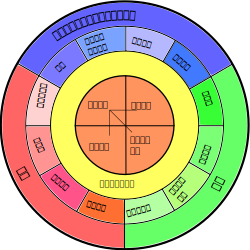
\includegraphics[bb=00 00 400 400]
{img/fig1.1.pdf}
\caption[空泡基础研究间的链接]{空泡基础研究间的链接(翻译自文献)。从理论到设计到应用的三层关系。\cite{blake_cavitation_2015}}
\label{fig1.1}
\end{figure}




空泡动力学是一个具有物理和工程意义的主题。在空泡生成的瞬间,因其位置处产生相变,相变后的气体具有极大的压强,因外界液体环境仍保持较低的原液体压强,从而使气体急剧膨胀。在这个瞬间,压力向外传导,形成一种压力间断,即空泡在诞生瞬间向外辐射一个冲击波。这个冲击波在液体环境中传播时逐渐衰减,并形成对外的力学作用。空泡受初始内部高压驱动而膨胀,直至空泡达到最大泡半径,此时空泡的内部压力为气体分压加水蒸气的饱和蒸汽压。随后空泡在外内压差驱动下而收缩。这个膨胀收缩的过程中,也会对周边形成力的作用。在空泡收缩时,其终末速度极高,形成撞击时其压力和温度可以达到非常高的程度,会向外将撞击的能量辐射出去。在空泡的球性极高时,撞击的体积及体积的表面积更小,足以形成特殊的声光效果——声致发光(sonoluminescence),甚至曾有猜测可以达到核聚变温度。人们在物理和数学层面认识了空泡动力学过程,并将其应用到了实际生产活动中\cite{Prosperetti2017}。空泡的产生方式通常采用电火花,激光,微炸药等方式激发,或者产生静态张力泡。


激光作为一种直接、高效的能量传输方式,其频率高、方向性强、能量集中,在上个世纪60年代被发明后便受到来自学界、军事和工业界的普遍而迅速的关注。随着时代的进步,高能激光与原子分子的相互作用机理逐渐清晰,激光作为能量传输载体的功能逐渐得到广泛的应用,如材料的切割、损伤、光刻,熔融成型等。激光导致的能量沉积型相变也在物理和实践中吸引了热烈的目光,特别是利用激光击穿液体的方式构建空泡,因其非接触性和极好地可控性已经成为研究空化气泡最为普遍的产生方法。短脉冲激光聚焦位置形成极高的电场强度,当其超过当地的击穿阈值时,使当地水分子发生逆韧致辐射,击穿当地液体团,并形成等离子团。这个光致电离过程涉及到多光子电离、碰撞电离、雪崩电离和隧穿电离等多个过程\cite{li__2022,__1996}。通常因为时间尺度差距较大,在研究空泡动力学时,只将其形成的等离子团在复合后的高温高压气体团作为空泡的初始阶段而不考虑其具体的击穿过程。这样就可以获得较为理想条件下的空泡动力学。同时激光强度在没有达到击穿阈值时也可以形成空泡,即利用激光的热效应,使水在当地气化即沸腾,从而形成一个高温高压的初始气泡团。通常这样的空泡多发生在界面附近,或使用长脉宽激光作为热源的情景中。

激光诱导产生的单空泡和较小数量的多空泡研究是空泡动力学研究的基石。通过理解单空泡和小数量的多空泡的运动特性,对理解空泡群体行为和将其应用具有关键的基本作用。特别地,在实际应用场景中,空泡往往不是孤立出现,而是伴随着各种约束条件,比如界面和力的作用。理解空泡在复杂力学环境内的运动是一项兼具科学和工程意义的课题。

%\section{研究现状及进展}

\section{国内外研究进展及现状}


\subsection{激光诱导击穿等离子体}
激光本质上是一种电磁波,其在一般意义上通过其电场与物质的分子原子结构进行相互作用。对于击穿中涉及的液态水的电离机制,大致可以分为强场电离与级联电离。而其中强场电离也可以分为两类:一类是束缚态电子连续吸收离散数目的光子跃迁至电离自由态的多光子电离;一类是电子隧穿通过原子库伦势与瞬态光电场的叠加势垒的隧穿电离。

1966年,G S Voronov\cite{voronov_multiphoton_1966}利用红宝石激光器辐射强电场中氙原子对气体中多光子电离展开研究,实验中发现对于在~107 V/cm 的强光场中,电离的有效性与光子束强度成正比,并且使用微扰理论的数值计算给出了电离概率的数值解。1968年,P Agostini\cite{agostini_multiphoton_1968}等人利用400MW的钕激光聚焦在一个充满惰性气体的真空室中,通过绘制离子数量与通过焦点的光束功率对比图,给出了一个原子同时吸收的光子数的数量,并且阐明了实验上光子数量的值与理论上值的差异,为后面的多光子电离研究提供了重要的理论依据。 随后,在1972年Michael\cite{bass_avalanche_1972}等人通过研究不同的材料表面损伤概率与功率密度的关系,并对这一现象进行了说明,首次提出了雪崩电离也可能是激光诱导击穿的重要原因。1981年,M. Sparks\cite{sparks_theory_1980}对固体中的电子雪崩击穿进行了理论解释,并且通过实验证明了理论的合理性的同时还获得了雪崩击穿与温度,激光脉宽,波长以及不同材料之间的依赖性,同时该理论在波长长于$1\mu m$情况下,无法正确地描述材料间的击穿现象,还必须考虑多光子吸收。

多光子电离可以分为共振跃迁和非共振跃迁两种。共振跃迁多光子电离是指原子依次吸收能量不同的数个光子,并且每个光子的能量和跃迁能级差相等,也就是原子发生跃迁时都能进入其能量本征态(即电离过程中实际的中间能级)。在实验上可以通过可调谐染料激光器激发原子实现共振跃迁多光子电离。另一种情况是原子吸收的光子能量后并未进入原子的中间能级,反而进入激光诱导的虚能级。这种跃迁不需要任何中间本征态,这通常是强激光与原子相互作用过程。由于虚能级的寿命通常很短( 或以下),所以要求激光在超短时间内产生足够的光子数才能充分激发非共振跃迁多光子电离,因此多光子电离通常需要较强的光场才能显现出来。多光子电离速率可以表示为 $W_{MPI}=\sigma_KI^k$,其中,$\sigma_K$为K个光子的电离截面,I为激光光强。

当强光场的峰值抵达原子系统时,原子的库伦势的一侧将会被明显压缩,此时电子通过右侧势垒隧穿的概率明显增加,电子波包将以一定的概率隧穿至原子势垒外侧形成电离。考虑我们现阶段研究涉及的内容,主要机制是多光子电离以及雪崩电离,此处对隧穿电离不再赘述。

当一个价带电子连续吸收离散数目的光子跃迁至边缘导带,随后通过多次逆韧致辐射机制吸收光子,从而进一步获得能量跃迁至临界导带,成为自由电子并与其他中性分子碰撞发生次级电离,额外产生一个低能的自由电子。之后,两个低能自由电子重复上述吸收光子的过程,生成四个自由电子,重复上述过程将会最终引发雪崩过程(即级联电离),造成激光汇聚区域电子数密度迅速增加,形成击穿。
相应的级联电离速率为:
$$\eta_{casc}=\frac{1}{1+(\omega\tau_c)^2} (\frac{e^2 \tau_c I}{cn\epsilon_0 \Delta Em}-\frac{m\omega^2 \tau_c}{M})\,,$$
其中,M为中性分子的质量,$\tau_c$为自由电子和分子碰撞平均所需要的时间间隔($\tau_c=1fs$),$\varepsilon_0$为真空中介电常数。在光学击穿产生等离子体的过程中,影响电子密度变化率的主要因素有:多光子电离,雪崩电离,电子的衍射扩散以及电子复合。前两个是增加电子密度的因素,后两项是减少电子密度的因素。

1995年,Kennedy\cite{kennedy_first-order_1995}将Shen\cite{shen_principles_2003}推导的简单速率方程和Keldysh\cite{fedorov_l_2016}推导的多光子电离率相结合,率先提出了在纳秒及以上脉宽层面广泛认同的,考虑了自由电子密度的全局演化的电子密度变化公式:
$$\frac{d\rho}{dt}=(\frac{d\rho}{dt})_{mpi}+\eta_{casc}\rho-g\rho-\eta_{rec}\rho^2\,,$$
其中第一项,第二项分别为多光子电离速率以及级联电离速率,已在上文中给出,对于上式中的$g$和$\eta_{rec}$分别表示的是:电子扩散出聚焦体积的速率以及电子的复合系数。对于脉宽$\tau\le10ns$时,通常会忽略扩散项$-g\rho$\cite{mlejnek_dynamic_1998,jarnac_whole_2014}且,当$\tau\le10ps$时,会将电子扩散以及复合项都忽略\cite{lenzner_femtosecond_1998,tien_short-pulse_1999}。
对于扩散项g:设光束束腰为$\omega_0$,瑞利长度为$Z_R$:$Z_R=\frac{n\pi\omega_0^2}{\lambda}$,$$
g=\frac{\tau_c\Delta E}{3m}\left[\left(\frac{2.4}{\omega_0}\right)^2+\left(\frac{1}{Z_R}\right)^2\right]\,,$$
Docchio\cite{docchio_study_1988,noack_laser-induced_1999,docchio_spatial_1991}等人通过光谱分辨测量等离子体的光衰减,获得等离子体中的复合系数的一般值:
$\eta_{rec}=2\times10^{-9}cm^3/s$。
另一种多层的电子密度演化速率方程主要用于解释皮秒以下的击穿过程,此处不述。
由于本文的重点在于空泡的动力学,故对激光致水击穿的更多详细研究过程不再赘述。


\subsection{激光致空泡动力学研究}
激光致空泡在很多领域都有诸多研究,特别是水环境下的材料处理\cite{barcikowski_materials_2019},和生物光学\cite{vogel_working_1990,juhasz_corneal_1999,toytman_multifocal_2010,jang_optothermally_2019}。通常在激光能量沉积后,形成的高能量密度高温高压的等离子体,继而演变成具有高振幅的脉动空泡\cite{47ee882c1e5b8fc9b161bae7598dafe099ccb01e},并伴随一个演化成为冲击波的压力瞬态。空泡随后运动至溃灭,并形成另外一个冲击波\cite{liang_comprehensive_2022}。等离子体的大小通常可以通过其闪光来决定\cite{vogel_shock_1996}。自由域内空泡的生存周期可以通过光偏转法,这种方法可以获得精确到nm的空泡溃灭振幅。也可以间接的通过两次冲击波的时间间隔获得,当然最简单的通过高速摄影也可以获得。但这几种获得空泡生存周期的方法的精确度逐渐递减\cite{vogel_femtosecond-laser-induced_2008,schaffer_dynamics_2002}。高球性的空泡产生通过激光的紧聚焦获得\cite{venugopalan_role_2002,obreschkow_quest_2013}。对这种理想的高球形的空泡进行物理建模,在不同精准度和不同模型考量情况下有过很多尝试。

例如Rayleigh爵士提出的解释水中的真空孔洞形成的水的运动的模型,可以一定程度上解释空泡的溃灭进程\cite{rayleigh_viii_1917}。特别是通过这个模型而获得的Rayleigh时间,也就是半程空泡生存周期,为学界所通用。其表示为
$$T_C^{Rayleigh}=0.91468R_{max}\sqrt{\rho/p_a}\,。$$

Plesset和Gilmore以及Keller等学者不断修正和添加考量量,形成了现在广为使用的Gilmore修正的Rayleigh-Plesset模型和Keller-Miksis模型\cite{Gilmore1952,plesset_collapse_1971,keller_bubble_1980,vogel_cavitation_1986,lauterborn_experimental_1975}。同时也存在着基于Rayleigh-Plesset的半经验工程模型,添加拟合常数以获得较好地拟合效果\cite{zhong_model_2020,e8c740d030b19350fce6133360d2ed165a59bd78,supponen_shock_2017,supponen_collapse_2017,obreschkow_analytical_2012,welch_pulsed_2010,selmke_bubble_2020,lohse_bubble_2018,long_early_2020}。
\bigskip
\medskip
\subsubsection{激光致空泡机制}

使用激光击穿时,激光系统的多样性,造成了空泡初始状态和后续动力学的多样性。Y.Tian和Tagawa等发现提升激光聚焦角度能极大地减小多点击穿的概率,特别是在聚焦角度大于29.8°以后,在适当的能量范围内多点击穿很少发生\cite{tian_stabilization_2016,5cc135338ea245a01dafd12d44f183533dca487e,tagawa_pressure_2016}。激光脉冲能量的提升使多点击穿的概率提升\cite{kennedy_laser-induced_1997},同时液体存在的杂质\cite{3d66d01b44fd4e7e6a8da70ed5dd2de9fca0dfac},击穿的概率发生特质\cite{kennedy_laser-induced_1997},像差\cite{evans_lens_1969,2b9cbf597962b6d717ea63693143471a76669358},等离子体的逆光生长\cite{docchio_study_1988},自聚焦\cite{potemkin_highly_2015,evans_pump-probe_2010}等都影响多点击穿的发生。多点击穿发生时,每个等离子体并不是同时发生的,而是以与焦点距离增加而变慢的\cite{docchio_study_1988, capon_nd_1988}。Evans等人\cite{evans_pump-probe_2010}发现当多个等离子体形成时,会产生多个空化气泡和冲击波。由于低密度等离子体诱导的额外气泡的形成,初始气泡和冲击波的数量有时超过等离子体的数量\cite{5a91d410705767266bdb87527d785a319238fdbf}。F.V.Potemkin等研究了透镜像差形成的长击穿和多点击穿,结果发现大数值孔径会导致击穿长度变长,进而形成更长的空泡\cite{potemkin_dynamics_nodate}。他们还利用这种长空泡产生了圆柱形冲击波前\cite{potemkin_laser_2014}。JING WANG等发现,空泡生存周期、初始冲击波远场峰值压力和相应的等离子体体积之间存在线性依赖关系\cite{fu_experimental_2018}。空泡聚合对主空泡的生存周期影响很小,但溃灭冲击波的强度和随后空泡的反弹受到很大影响,即多点击穿会抑制空泡能量转化为溃灭冲击波能量,但会增强转化为反弹空泡能量。
在多点击穿后形成的多空泡机制有可能在多个领域中发挥作用\cite{peters_highly_2013}。

关于激光击穿等离子体,也有在更复杂的激光条件和更复杂的水环境的研究。比如A. Young, 等研究了重频脉冲激光击穿水形成空泡的过程,发现激光击穿后其形成的影响在水中可以遗留达到一秒钟以上。因水中包含微泡和粒子,其会造成击穿冲击波的加强,等离子体产生位置会发生前后变动,等离子体形态也会发生改变\cite{young_laser-induced_2021}。YE TIAN,等研究深海高压环境中激光击穿产生等离子体,发现外界高压急剧减小了空泡生存周期,这使等离子体从溃灭中获得能量,提高其辐射强度,但在空泡溃灭后会立即溃灭\cite{tian_laser-induced_2020}。

当激光入射到特殊的靶材上,比如金、铂、铝等表面材料或颗粒,其光强不足以击穿水或者靶材时,这些靶材吸收光能,并转化成其内能,形成局部的过热点,从而形成沸腾机制的空泡\cite{welch_pulsed_2010,venugopalan_thermodynamic_1996,miotello_critical_1995,venugopalan_effect_1994,miotello_laser-induced_1999}。这种空泡的运动机制与击穿空泡在空泡生命周期尺度上没有差别。学界通常将他们的动力学过程混一而谈。本章中,将起归并到下文壁面附近的空泡和颗粒附近的空泡的段落中。
\medskip
\bigskip
\subsubsection{空泡的相互作用}\label{chapter1.2.2.2}

解释空泡间与各种边界相互作用时,通常会简单的采用基于势流理论推导的开尔文脉冲理论来解释\cite{Blake1987,zhang_unified_2023,blake_kelvin_1988,blake_cavitation_2015}。开尔文脉冲定义如下:
$$\bm I=\rho\int_{s}\phi ndS\,,$$
$\rho $是液体密度,$\phi$是速度势,$ S $是空泡的表面积,$n$是自液体指向气泡内部的法向模矢量。为了更加经验的简化理解空泡与其他边界条件的相互作用,还定义了一个无量纲常数:
$$\bm{\zeta} \equiv -\nabla p R_0 {\bm{\Delta}} p^{-1}\,,$$
其中的负号是为了保证射流和${\bm{\zeta}}$的方向一致。${\bm{I}}$ 和${\bm{\zeta}}$ 之间存在如下关系:
$${\bm{I}}=4.789R_0^3\sqrt{\Delta p \rho}{\bm{\zeta}}\,,$$

我们获得一个简单的用于判断各种场情况下的空泡和射流运动的参数表如下\cite{supponen_scaling_2016}:


$$\bm\zeta=-\rho \bm g R_{0} \Delta p^{-1} \quad \text { 重力场, }$$
$$\bm\zeta=-0.195 \gamma^{-2} \bm n \quad \text { 固体平面, }$$
$$\bm\zeta=+0.195 \gamma^{-2} \bm n \quad \text { 自由平面, }$$
$$\bm\zeta=-\rho(\bm u \cdot \bm \nabla) \bm u R_{0} \Delta p^{-1} \quad\text { 稳定势流, }$$
$$\bm\zeta=0.195 \gamma^{-2}\left(\rho_{1}-\rho_{2}\right)\left(\rho_{1}+\rho_{2}\right)^{-1} \boldsymbol{n} \quad\quad \text { 液体界面, }$$
$$\bm\zeta=0.195 \gamma^{-2}\left(4 \alpha-1-8 \alpha^{2} e^{2 \alpha} E_{1}(2 \alpha)\right) \bm n \quad \text { 惯性界面。 }$$

这里的$\bm u$是速度场,$\rho_x$是不同液体的密度,$\alpha$ 是一个有关密度距离和表面密度的量,$E$是一种指数积分函数。一般的,$\bm{\zeta}$可以用来判断溃灭的激烈程度和射流的方向:当$\bm \zeta\le{10}^{-3}$时,产生弱的相互作用,和弱的射流。$\bm \zeta>0.1$ 时产生强的相互作用,和强烈的射流冲击现象。中间的过渡值则产生中等程度的溃灭。
额外地,这个量还可以用来量化更多的空泡溃灭过程中存在的量:

$$ \Delta T_\mathrm{jet} / T_\mathrm{collapse}=0.15 \bm{\zeta}^{5/3}  \qquad \text{归一化的射流撞击时间}$$
$$ U_{\mathrm{jet}}/(\Delta p /\rho )^{1/2}=0.9\bm \zeta^{-1} \qquad \text{归一化的射流速度}$$
$$ \Delta z / R_0 =2.5 \bm \zeta^{3/5}\qquad \text{归一化的空泡移动距离}$$
$$V_\mathrm{impact}/V_\mathrm{max}=0.11\bm\zeta^2 \qquad \text{归一化的射流撞击时的空泡体积}$$

用来解释空泡间相互作用的理论还有也是通过势流理论和Rayleig-Plesset模型推导出的二阶Bjerknes力\cite{harkin_coupled_2001,mettin_bjerknes_1997}:
$$\langle F_1(t)\rangle=\dfrac{2\pi\rho\Omega^2R_{10}^3R_{20}^3}{D^2}\delta_1\delta_2\text{cos}(\varphi_1-\varphi_2)$$
通常其用来解释两个空泡间的吸引和排斥,此处不再详述。

\medskip
\bigskip
\subsubsection{空泡运动的模拟}

当前对空泡运动主要数值模拟方法多种多样,有基于有限体积法的VOF法\cite{lauterborn_bubble_2018,koch_numerical_2016},边界元法(BIM/BEM)\cite{klaseboer_simulations_2006,Kim2014}、格子玻尔兹曼方法(LBM)\cite{shi_numerical_2019,chen_experimental_2023,gupta_lattice_2008},光滑粒子流法(SPH)\cite{zhang_sph-bem_2019,zhang_sph_2015,wang_axisymmetric_2022},以及分子动力学(MD)\cite{shih_effect_2020},此处不再穷举\cite{ohl_shockwave_2013}。

但非常突出地,数值模拟存在一个多物理场耦合的问题,也就是通常关注空泡动力学过程的模拟研究的初值设置是经验性的。激光击穿的时间尺度通常在纳秒甚至飞秒,已有的研究能够很好的获得等离子体过程\cite{zhang_transient_2016}。在其后的等离子体分离和空泡脉动的过程因空间和时间尺度与等离子体过程差距较大。而且采用有限元方法对流体的模拟仍存在无法准确捕捉流体变形,计算量大和守恒难等问题。对两个阶段的过程的衔接仍存在着不可克服的问题。一个很有意义的尝试是赵旭宁和Kelvin Wang利用水平集和相变规则结合,将未达到击穿阈值的激光辐射用能量转化方程处理成一个脉宽热原,求解全过程的Navier-Stokes方程\cite{zhao_simulating_2023}。他们的研究能够同时且准确地描述激光辐射、气化、和后续的空泡/流体动力学过程,其计算精度达到二阶。更近一步地,基于物理辅助的机器学习的模拟方法也正在成为新的关注热点\cite{wang_machine_2021,zhai_predicting_2022,zhai_bubblenet_2022}。


\subsection{空泡受特殊力学环境影响的研究}
空泡在自然和工程应用中,往往不是孤立存在的,而是倾向于以丝、条、团簇、和云等形式存在于不同的液体环境中。下文中将以特殊环境为主题梳理空泡研究的现状。本作中将这些特殊力学环境大概的分为:多空泡间相互作用、空泡与多种界面相互作用、空泡与压力波相互作用、和空泡云及空泡成核等。
\medskip
\bigskip
\subsubsection{多空泡}
通常在多空泡的研究中,是基于一个所有空泡都独立的遵从Rayleigh-Plesset模型的假设,研究空泡群体的整体性质,但实际上,空泡往往不是独立的,而是相互影响的\cite{__2022,blake_bubble_1999,lauterborn_physics_2010,blake_acoustic_1999,Biesheuvel1984,zhang_ensemble_1994,fuster_modelling_2011,arora_effect_2007,servant_interaction_2003,johnsen_shock-induced_2008,betney_computational_2015,lauterborn_acoustic_2007}。多空泡系统中,空泡的形状、大小、生命、脉动、平移会产生不同于孤立空泡的变化。多空泡的研究可以大体分为有序排列和随机分布的两种情况。随机分布的研究,往往通过某种平均来获得多空泡间的能量集聚,空泡的侵蚀作用,空泡的噪声等。有序排列则实现简单且能具体到单个泡的动力学。泡间相互作用可以简单理解为空泡在另一个空泡的辐射声场中的运动。这种相互作用使同相的空泡相互吸引并减速溃灭,异相的相互排斥并加速溃灭。同时泡间相互作用也会改变空泡的形状,并且使空泡不均匀收缩而产生射流,由于不同距离不同相位产生的射流方向和动量也不同。多空泡场景下,空泡的最大泡半径和生存周期与孤立单空泡发生较大改变,外围和内部泡的表现也存在明显的差异。 在多空泡阵列中,相近的空泡相互改变了环境压并能够起到屏蔽作用。整个过程会持续的比孤立单空泡情况更久。通常,相比于内部空泡,边缘空泡能达到更大的尺寸,并且更快的溃灭,并且在收缩过程中形成从边缘指向内部的射流。而内部空泡在空泡阵列平面这个维度上受到相邻空泡的限制。它们的动力学演化被相邻空泡和另外的自由维度控制。 

最基础的,对多空泡的研究的开端是双空泡系统。早在1971年,Shima等人便基于球形假设研究了双空泡系统的共振频率(自然频率)\cite{shima_natural_1971}。他们发现双空泡系统自然的有两个自然频率,并且受距离和空泡大小的影响。后来Shima 还研究了双空泡系统在固体边界的运动\cite{shima_behavior_1992}。并得出固壁面会使球形空泡生存周期延长的结论。2001年,Harkin等人利用二阶Bjerkness力理论解释了双空泡的脉动和位置移动\cite{harkin_coupled_2001}。2009年Siew-Wan、Quinto-Su 、CD Ohl、B.C. Khoo等实验的研究了同相异相/同大小异大小的空泡间的相互作用\cite{fong_interactions_2009,quinto-su_interaction_2009,chew_interaction_2011}。他们总结了强、中、弱等多种相互作用强度和多种射流发生方式:同向,相向等。并用Rayleigh理论解释了泡间的相互作用。

Shen Yang 等理论的研究了双空泡系统通过声辐射相互影响而导致的理想球形空泡径向半径的变化规律\cite{shen_role_2021}。研究表明空泡能被彼此压缩或拉长,其效果取决于外界驱动声波、空泡半径、空泡距离、和空泡数目。2015年,韩冰总结以往双空泡的实验并结合Lauterborn已有研究,模拟研究了双空泡情境下的各种组合\cite{han_dynamics_2015}。反相双空泡系统中产生的射流比其他情景下都强、快、长,而且这个射流的方向是可控的。并且模拟的获得了两张关于射流速度的map图,以讨论双空泡系统参数对射流速度的影响。代表性地,国内的张阿漫、崔璞、李帅等系统地研究了双空泡系统,包括双泡系统的接合、移动、破碎、射流和冲击波激发以及变边界脉动\cite{han_experimental_2018,li_experimental_2019,wang_jet_2019,cui_experimental_2020,liu_interaction_2021}。

对双空泡系统的研究帮助展开了更进一步地多空泡相互作用的研究\cite{prigogine_experimental_2007}。多空泡往往对空泡的排布方式较为关注,一般地会形成特殊的阵列方式,如线形,面形,环形等组合。本文作者研究了三个线性对称排列的同相空泡,利用DOE三点分光镜获得等能量的激光脉冲,从而在自由水中同时地激发三空泡阵列。发现在线阵中中间空泡的多种溃灭方式,类比了空泡阵列和单空泡的溃灭逻辑,形成了对线性同相等大小空泡阵列的认知\cite{bao_experimental_2021}。后续陈荣等继续了异相线性三空泡的研究,对形成了对相位造成的射流的更多认识\cite{chen_experimental_2022}。
J.P. Dear,等在1988年通过在凝胶(gelatin)中创建静态张力泡的方法,研究了多种空泡阵列在受压力波作用后的溃灭形态,发现了屏蔽作用的存在\cite{Dear1988a,dear_study_1988}。Bremond、Ohl和Lohse等人利用壁面挖孔作为空化核,利用负压形成空泡的方法,研究了空泡阵列在壁面附近的脉动,并用Rayleigh模型和边界元方法进行了解释\cite{bremond_interaction_2006,bremond_controlled_2006}。Lauer等开发了一种界面追踪的数值算法,用来研究了冲击波对一个空泡阵列的作用。很好的验证了空泡的屏蔽,击穿和相互作用\cite{lauer_numerical_2012}。Matevz 等研究了相邻蒸汽泡对沸腾热流的影响,其通过在平板上设置多个空泡腔,并用沸腾的方法制造多空泡,发现空泡在不聚合的情况下导致的外流动只影响了较小的范围\cite{takeyama_influence_2021}。Ochiai等研究了多气泡在声压下的动力学,其溃灭表现出与空泡阵列近似的压力辐射\cite{ochiai_numerical_2017}。Tiwari等研究了一个空泡团簇在壁面附近的集体行为\cite{tiwari_growth-and-collapse_2015}。

Haiyan Chen利用二阶Bjerkness力理论解释了多空泡的脉动\cite{chen_modulation_2020}。张阿漫等也针对多空泡做了有益的探索,比如十字形和环形空泡的脉动\cite{zhang_interactions_2023}。Jian-Bo Li等研究了有不同形式排列的静态空气泡存在时的空泡溃灭强度,结果显示气泡与空化气泡相互作用的范围内,气泡与空泡的相对距离,大小和数量会极大地影响迁移方向,延长振荡时间和衰减溃灭声压,而且还产生了空泡被分裂成多个空泡的现象\cite{li_influence_2021}。秦玉鹏等理论的研究了多种空间排布空泡的动力学特性\cite{qin_analytical_2022}。Peng-li Zhang等数值的研究了更长的线性阵列组合\cite{zhang_study_2019}。多空泡的排布,内容物,边界条件的变化不一而足,此处不再详列。
\medskip
\bigskip
\subsubsection{空泡与多种界面相互作用}

空泡间的相互作用只是空泡受特殊环境影响的一个方面,更多的研究是空泡与不同形式的界面的相互作用过程\cite{Prosperetti2017,lohse_bubble_2018,lauterborn_physics_2010}。

比如空泡在水气界面,其溃灭时往往形成射向空气中的长射流,其已经获得几十年的研究\cite{boulton-stone_gas_1993,krishnan_scaling_2017,deike_dynamics_2018,e2863fbdabad074393d8ced60bcea666015f76db,6eb937979b9271fc82586961a0a59db1a3bac47c,li_bubble_2019,03a7e1892c909c181fa4619ef2eb9ea70084e02f}。因与界面的距离不同,表现出不尽相同的特性。但总的来说在膨胀时会形成液面向外的变形,并在收缩时因水的汇聚而形成射流。近期的,Juan 和CD Ohl等研究了不同曲率下的水气界面附近的空泡脉动,结果发现在靠近水气界面的空泡形成向上的射流时,同时也形成了向内的射流。这个向内的射流速度可以达到40m/s,最远可以达到15倍的空泡半径\cite{rossello_dynamics_2022}。同时在水平界面附近,这个反向射流是指向重力方向,而在曲率界面附近,张力导致的这个射流更偏向其几何中心。

同时空泡在液-液界面附近,也可以看成一种近似自由界面的动力学过程。该研究的最初动机是对液体超声(空化)制备乳液的背景有更深入的了解。Matevz等研究了液-液界面附近空泡动力学以了解界面的变形和指进,结果显示空泡产生在较轻的液体中时,空泡产生的射流将指向界面,但如果空泡产生在较稠密的液体内部,则空泡射流远离界面\cite{orthaber_cavitation_2020}。Brujan研究了空泡在gelatin附近的动力学过程,并着重的理解了杨氏模量的作用\cite{brujan_dynamics_2001}。

空泡与固体界面的相互作用因其应用广泛,是最受学界关注的方向。Blake,Brenen,Lauterborn,Prosperetti,Lohse等人都对这个主题进行了充分研究\cite{lohse_bubble_2018,lauterborn_physics_2010,blake_interaction_1993,brennen_cavitation_1995,Prosperetti2004}。
比较具有代表性的是,水下炸弹爆炸损伤船体。其过程可以大致分为三个过程:1.相变及其冲击波。冲击波相对空泡壁面具有更高的速度,在相变失去后续能量补充后的一段时间内与空泡分离。这个冲击波经水体传播后至船体,冲击波对船体形成应力损伤。2.空泡脉动。当空泡在水中持续膨胀以释放内部高压时,对固壁面形成压迫和推动。特别是在船体尺寸相对空泡尺寸不具有压倒性的尺度时,空泡的膨胀足以推动船体脱离水面。在这个过程中,因为空泡的不均匀推动和自身重力影响,会持续加重船体的应力损伤。同样的,空泡在收缩时也产生相似的机理。3.空泡溃灭冲击波和射流。空泡在完成膨胀转而收缩时,外界水体在空泡内外压差的驱动下,推动空泡收缩。由于水体的惯性,在空泡溃灭时,向外释放出水锤压力。此溃灭冲击波对船体的损伤机理类似于相变冲击波。由于在船体附近的不均匀受力,空泡在收缩时会形成指向船体的射流。此射流头部具有高速,低截面面积的特征。其可以对船体形成明显的贯穿伤害。在这个典型案例中,涉及到不同的固壁面尺寸与空泡尺寸,固壁面与空泡距离等情景,其机理涉及到空泡的推动效应和固壁面应力等。
近期地,Lechner等数值的研究了空泡在固壁面附近不同距离时形成的射流,结果显示了在不同距离下显示了两种不同的射流方式,在小距离时因空泡接触固壁面会产生特殊的针样溃灭射流,而粘度会改变这个阈值距离,同时粘度越大,射流的速度越大\cite{lechner_jet_2020,lechner_pressure_2017}。

Jia-yun Zhang等实验和数值的研究了固壁面附近激光诱导空化气泡的溃灭\cite{zhang_experimental_2022}。通过使用照明光多次曝光技术,获得空泡壁面速度。结果表明,靠近壁面的空泡溃灭成轴对称的心形,指向壁面的微射流将空化泡拉向壁面。反弹阶段产生的反射流将驱动空泡远离壁面。其中射流的速度能达到一百米每秒。

Mandeep等发现空泡的溃灭 动力学取决于其在溃灭瞬间与固壁面的接触角\cite{saini_dynamics_2022}。并通过构建正负相对距离的情景,实现了不同的接触角。当接触角小于$90^{\circ}$时,观察到的是指向墙壁的经典射流,而如果初始接触角大于$90^{\circ}$,则出现平行于墙壁的环形再入射流。这种行为的变化可以用小时间的脉冲势流理论来解释,该理论表明当接触角大于$90^{\circ}$时,在接触线的初始加速度上存在一个奇点。脉冲势流理论很好地反映了最大膨胀瞬间的空泡几何形状对整个溃灭过程的作用,该理论可以很容易地推广到其他空泡形状。

Zibo Ren等研究发现附着在固壁面表面的微纳气泡不直接响应空泡的拉伸应力,但是会被射流引起的剪切流影响而形成系链式结构,以至于分裂出更小的气泡\cite{ren_strong_2021}。
Jiayang Gu等研究了空泡冲击固壁面情况下的空泡动力学,研究了空泡与固壁面的相对距离对三种激光空化冲击(LCP)作用机制即激光冲击波,空泡溃灭冲击波和水射流的影响\cite{gu_bubble_2021}。相对距离越大,固壁面收到的冲击波强度越大,但射流越弱。他们获得了一个针对Q235钢表面硬化的最佳相对距离$\gamma=0.4$。

Jiangyou Long等使用高分辨率的频闪式阴影成像系统观察并研究了在脉冲激光烧蚀钛靶材在不同液体环境中产生的空化气泡的早期演变\cite{long_early_2020}。提出了一种流体动力学模型来计算气泡内和周围流体中的早期压力变化。结果表明,空泡是一个在初始阶段后被高压流体层所包围的低压区域,其演变主要受液体密度的影响。其演化主要受液体密度的影响。在高粘度液体中,初始气泡压力显著增加。

XiangLu等研究了空泡溃灭导致射流撞击固壁面的冲击载荷\cite{lu_equivalent_2021}。基于微射流理论和液固冲击的水锤效应,在变形等效原理下建立了单个空泡破裂微射流的冲击载荷等效模型。由于可以认为空泡均匀分布在足够小的区域内,基于单个空泡冲击载荷的等效结果,可以推导出多个空泡破裂微射流在微段内的冲击载荷等效模型溃灭微射流。形成了单个和多个近壁声泡破裂微射流空化损伤加载的等效方法。验证结果表明,这种等效冲击载荷具有极高的准确性。

Pu Cui和张阿漫等研究了利用空泡溃灭的破冰的研究,包括单空泡和双空泡的情景\cite{cui_experimental_2020,cui_ice_2018}。当单空泡作用时,冰板从顶部诞生裂缝,即从冰-空气界面发展。这归因于冲击波在界面上的反射引起的张力。当冰板的厚度或空泡-冰的距离增加时,这种断裂会减弱。当空泡-冰的距离足够小时,在冲击波入射时也可能从冰板底部形成断裂。空泡形变和冲击波也能推动冰板的运动。双空泡作用时,观察到独特的空泡行为,包括合并、分裂、倾斜的反射流和不对称的环形空泡溃灭。测量了研究了空泡动态特性,例如射流速度、射流能量和气泡中心位移。在一系列空泡间和空泡-边界距离情境下,使用压力换能器测量了两个空泡的冲击波辐射,表征了其破冰能力。他们发现在多种组合的情况下,通常在冲击波减弱时其损伤效果会同步的减弱。Gregorčič等还研究了空泡在固体边界和自由界面间的动力学\cite{Gregorcic2007}。讨论了生存周期受自由界面缩短和硬边界延长的两种效应。

在更工程的层面理解空泡与固壁面的相互作用,自然而然的会谈到空泡的侵蚀和清洗作用。Fabian和CD Ohl揭示了在空化气泡的非球形坍塌过程中导致能量集中并最终导致硬化金属腐蚀的决定性机制\cite{reuter_cavitation_2022}。研究表明,只有在非轴对称的能量自聚焦情况下,接近金属表面的环境压力下的单个空泡才会引起侵蚀。空泡在溃灭时首先在一点汇聚,并产生冲击波,其他残余气体形成被这个冲击波强化的溃灭。同时他们还证明了只有在相对距离足够小时($\gamma<0.2$),硬质表面才会产生侵蚀。常规射流即使达到100m/s,也没有造成损伤,因此他们建议,在需要考虑减小损伤的情况下,空泡形成射流时要同步破碎,以防止产生针状射流和不对称自聚焦。反之也可以加强损伤。Fabian等人开发了一种利用空泡损伤铝制材料表面氧化膜形成的导电性能变化来计量空泡损伤效果的方法,这种方法具有以微秒分辨率,非侵入性、就地实时的优点\cite{abedini_situ_2023}。其在靠近铝样品表面的 NaCl 水溶液中产生单个激光诱导气泡。高速计时电流法用于记录样品和浸入相同溶液中的相同铝电极之间流动的腐蚀电流。这种配置使得可以通过再钝化产生的腐蚀电流来测量铝表面纳米薄钝化层中的空化损伤。与腐蚀电流与同步的高速成像记录之间的相关性允许对空泡动态的各个阶段造成空化损坏进行计量。对于最小的初始相对间距,观察到最大的空化感应电流。随着空泡在几个阶段中重新膨胀和再次破裂,检测到更多的电流峰值,这意味着一系列较小的损坏。在中间距离处,空泡不会造成破坏,而在较大的距离处,空泡只会在第二次发生在固体表面的溃灭期间造成破坏。Park等对比了气体泡和水蒸气泡在超声场的驱动下对硬质表面的清洗效果\cite{park_comparing_2021}。研究发现气体和蒸汽空泡在超声场中表现出不同的动态行为,蒸汽空泡和气泡分别能更有效地去除附着力强和弱的污染物,此外,蒸汽空泡能更好地清洁疏水性基材。

激光照射材料靶材,其形成的纳米级材料喷溅,是当前生产纳米粒子的一种通用方法。在这个过程中产生的空泡和粒子的相互作用也引起了很多兴趣。特别是人们发现,可以利用空泡来驱动粒子实现特定的运动时,许多研究者对激光与颗粒的相互作用的过程进行了研究。

Liang Lv和Yuning Zhang等实验研究了空泡与颗粒距离对近似大小的空泡与悬挂颗粒相互作用的影响\cite{lv_experimental_2019}。研究发现近距离排斥和远距离吸引的机制。远距离吸引可以用辐射压力来解释。近距离排斥则可以用射流来解释。Xiaoyu Wang 和Yuning Zhang实验的研究了球形粒子附近的激光诱导空泡的动力学\cite{wang_theoretical_2022}。并用Weiss定理获得了开尔文脉冲理论模型。他们发现只有在相对距离γ>0.5时,空泡能较好的保持球形时才能使用开尔文脉冲模型解释空泡行为。颗粒对空泡与颗粒之间液体流速的影响主要受几何上空泡在颗粒的镜像位置影响,这块区域的液速总是低于周围其他区域。而空泡的中心移动可以用开尔文脉冲预测,并宣称了一个所谓的常数来获得开尔文脉冲与速度的线性关系。同一团队的Xiaoxiao Zheng 则实验的研究了两个相同尺寸的球形颗粒附近的空泡动力学\cite{zheng_investigation_2023}。他们认为开尔文脉冲理论模型能够有效地预测两个相同尺寸粒子附近的空泡的运动特性。当空泡初始位置沿水平对称轴逐渐远离两个大小相同的粒子附近的粒子时,第一周期空泡质心的移动距离先增大后减小。当空泡质心的初始位置在两个粒子附近的不对称位置时,空泡质心的运动方向偏向离空泡较近的粒子,而不是偏向该粒子的中心。

Linglong Wang等用高速全息显微术对激光诱导空泡进行了成像研究\cite{wang_measurement_2021}。他们发现不同尺寸的纳米空泡的脉动具有细微的差别。这种差别在归一化并平方后显示出与空泡半径的相关性。其结果表明,空泡的半径越大,脉动的进程越快。这是由空泡传热过程改变引起的。

Matevz同样研究了空泡在球形颗粒附近的动力学,以期解释微纳空泡杀菌的作用\cite{zevnik_cavitation_2022,zevnik_cavitation_2020}。结果中讨论了射流、冲击波、剪切力和热效应。并考虑到表面张力在小尺度上会引起的射流减弱效应。球形颗粒上的机械载荷倾向于随着球形-气泡尺寸比的增加而增加,并随着它们的距离增加而减少。他们还给出在溃灭末期,空泡对颗粒的压力影响可以达到$100 MPa /\mu m$的梯度。

Chunhui Luo  等研究发现利用激光空泡降解悬浮液有机物时,激光能量的提升对降解效果的提升在一定范围内是线性的,但在能量过高后等离子体的吸收效应会限制空泡生长,导致其有一个平顶式增长。同时发现,固体颗粒物在超过一定范围后浓度越大,激光空泡形成的溃灭效应越弱\cite{luo_impact_2021}。而且在固体边界附近中的空泡降解效果更好。其原因作者没有探讨,但其理所当然的来自更剧烈地非对称溃灭形式的自我强化。

Shengji Wu和刘树红研究了在固体界面附近产生的激光空泡驱动球形粒子的动力学\cite{wu_dynamics_2021}。结果发现了当颗粒在远离固体界面和空泡端时,颗粒的移动主要受空泡膨胀的影响。当颗粒在空泡和界面之间时,颗粒的移动呈现出多种方式。但最主要的当粒子距离空泡足够近时,空泡膨胀才会推动粒子撞击固体表面。当颗粒恰好在空泡正下方时,即使空泡在膨胀时没有接触到颗粒,颗粒也会被射流加速到多倍于空泡膨胀推动的速度。

Sieber和Farhat等研究了在固体界面上布置了纳米颗粒的情景下,空泡与其相互作用的过程\cite{sieber_dynamics_2022}。结果显示当相对间距γ>1.3时,该动力学表现为空泡与固体边界的相互作用机制。当0.6<γ<1.3时,空泡在溃灭时会将颗粒举起并形成一个小堆,这个小堆的尺寸取决于空泡与颗粒的相对尺寸和相对间距。在相对间距足够小时,空泡在溃灭时会形成钟型图样,并形成一个微射流。但在所有案例中,空泡的生存周期都因为泡能用来驱动纳米颗粒而消耗,从而形成生存周期的缩短。

因为空泡在自然界中和工程应用中涉及到的环境情况多种多样,学者们关心和关注到的现象和潜在的场景也多种多样。于是,更复杂的空泡与环境的相互作用场景也不胜枚举,下面仅述几例复杂边界的研究。

Brujan等研究了激光空泡在相互垂直的两个固体壁面间的动力学。结果表明,这种空泡的行为及其依赖于泡沫与墙壁之间的距离\cite{brujan_dynamics_2018}。当空泡溃灭时,会形成一个倾斜的射流,射流指向更偏向距离更近的壁面,当距离相等时则指向中间。且空泡会朝着射流方向移动。而射流击穿空泡后,空泡形成环状结构。这个结构在里壁面较远时,沿着径向溃灭形成小空泡。当这个环状结构接触到壁面时,接触部分会沿着壁面迁移并首先溃灭。从而形成新月状残余。

Yoshiyuki Tagawa等研究了水气自由面和垂直固壁面附近的空泡\cite{kiyama_direction_2021}。通过理论预测和实验验证,成功的给出了一个射流倾角关于相对位置的模型。

Abboud研究了在一个固体壁面上的孔洞结构对激光空泡动力学的影响\cite{abboud_microjetting_2013}。研究表明,即使在存在孔洞的情况下,空泡仍形成了一个指向固壁面所在平面的射流,并且这个射流会通过这个孔洞。一般地,空泡膨胀会在通孔处形成快速流动,并产生次级空化。在空泡膨胀通过孔洞后,在收缩时,凸出的灯泡状结构会脱落形成小空泡,在溃灭时形成朝向主空泡的反射流。

Hendrik和CD Ohl等研究了激光空泡在固壁面上通孔上方时的动力学过程\cite{reese_microscopic_2022}。针对通孔的长度,宽度和形状,以及空泡的尺寸,液体的粘度,空泡与壁面的距离,做了具体的研究。研究发现了三种射流机制,正向,反向,以及针形射流。

利用空泡形成乳化液滴也是一个非常常见的应用\cite{raman_microemulsification_2022,nieves_ultrasound-assisted_2021}。空泡是乳液形成的重要机制。空泡取决于油滴的粘性而形成不同的喷溅状态。

Xianmei Zhang等研究了在液滴内形成的空泡的脉动和位置移动\cite{zhang_radial_2022}。他们通过将体积模量考虑进状态方程推导出一个液滴内空泡脉动的类Rayleigh-Plesset方程,并据此研究了这个空泡的径向脉动和位置移动,他们把形成这种特殊平动的机制归因于液滴表面的限制。

Jingzhu Wang等研究了夹在两个薄板间的液滴内的空泡引起的液滴Rayleigh–Taylor不稳定性\cite{wang_rayleightaylor_2021}。实验、理论和数值模拟都获得了三种独立液滴形态:喷溅、贯通、和稳定状态。并通过定义了两个参数来研究了这三种状态。而空泡第一次溃灭形成的射流方向,取决于液滴与空气界面的接触角。

Zhao Fang等人还研究了利用空泡形成的微射流将固体颗粒表面的油滴去除\cite{zhao_numerical_2021}。通常大空泡的对大团油滴的清洗效果较好,而小空泡则对狭小局部的油滴的去除效果好。

Jin-Jie Deng等研究了在静电场与超声场中耦合作用下的空泡脉动\cite{deng_dynamics_2021}。研究发现静电场中的空化阈值更低。电应力降低了表面张力,导致空泡趋于不稳定而加速溃灭。但同时也提高了最大泡半径也降低了最小泡半径。有电场存在的情况下,空泡的动力学更加剧烈。

Tomaˇz Poˇzar等研究了一个模拟眼球形状下的激光击穿空泡\cite{pozar_laser-induced_2021}。也就是在一个凹面结构附近形成激光击穿。激光冲击波和溃灭冲击波通过反射,在焦点处形成次级空泡。

Matej Senegac ˇnik等设计了一个悬崖式固体壁面,悬崖是一个直角,并将这个固体结构浸没在不同的液体介质中,而空泡在悬崖表面产生\cite{senegacnik_dynamics_2021}。研究显示,空泡快速膨胀形成的高速水流在悬崖外侧形成次级空化,并在空泡边缘到达悬崖边缘时,形成涡流再次进入空泡内部。提高液体粘度,可以防止这种再入。

Yuning Zhang 等也研究了这种悬崖式表面,但他们将空泡放置在角平分线的反向延长线上,而不是表面\cite{zhang_collapsing_2020}。研究发现,这种结构能够明显的延长空泡生存周期。当空泡距离角顶点较近时,空泡收到束腰式限制。但距离中等时,空泡溃灭时将形成橄榄状,并且向角顶点移动。

Qingyun Zeng和CD Ohl研究了由两个刚性壁为边界的薄液隙中的激光空泡和诱导射流的动力学\cite{zeng_splitting_2020}。研究发现液隙的相对高度和空泡处于液隙的相对位置,对空泡的动力学表现具有决定作用。他们发现了三种射流形式:空泡分裂后射向两边,直接射向最近的壁面,和射向远端壁面的转换射流。特别地,这种转换射流是因为空泡相对液隙足够大,在膨胀面接触远端壁面后形成的射流方向转换。只存在于某些极端情况,这个机制决定于液体粘性边界层。
空化在牛顿流体中得到了广泛的研究,在剪切稀化流体中的研究程度较低但很重要。Guillaume T. Bokman和Outi Supponen研究了水-玉米淀粉悬浮液这种剪切增稠流体中的空泡动力学\cite{bokman_cavitation_2022}。这种流体的一个有趣特性是,当应变率增加时,它们的粘度会增加,直到它们表现出类似固体的行为,甚至会破裂。由于空泡能够产生极端应变率,其受到剪切增稠流体行为的影响。文章用Keller-Miksis 方程解释了其行为。在实验过程中也观察到了空泡膨胀导致的液体的碎裂。

空泡与生物组织的研究,多利用不同浓度的凝胶Gelatine代替生物组织。

Kodama等研究了空泡在水-凝胶(water-Gelatine)边界附近的脉动\cite{kodama_cavitation_2000}。空泡倾向于向界面移动但不会产生射流。空泡的生存时间除了在小相对距离情况下,其他情况都被延长。但在凝胶内部可以检测到10Mpa以上的压力。Oguri等研究了激光致冲击波与空泡相互作用在凝胶里导致的次级空化现象\cite{oguri_cavitation_2018}。得出凝胶中的起始空化阈值约为-24Mpa,与水中差别不大。

Dui Qin 等研究了空泡在生物组织中的动力学和声辐射\cite{qin_nonlinear_2021}。他们通过数值地研究粘弹性组织中两个相互作用的空化气泡的径向和平移运动以及由此产生的声发射,发现在他们文章的条件下双空泡对大空泡的增强作用。随着距离的增加,抑制逐渐减小,其辐射声波出现谐波、次谐波、超谐波和宽带分量的逐步演变。随着周围介质弹性和/或粘度的增加,气泡的非线性动力学和平移运动均显着降低。郎骥和吴千红等研究了空泡导致脑损伤的过程\cite{lang_cavitation_2021}。在这项研究中,用人造透明头部替代物发现了当头部受到突然的平移冲击时,撞击位置突变引起空泡的形成和溃灭。他们发现,空泡在脉动过程中对大脑表面形成损伤,并向大脑内部传播冲击波。对大脑内部形成暗损伤。
\medskip
\bigskip
\subsubsection{空泡与压力波相互作用}


Blake 等研究了行波驻波对空泡的影响\cite{wang_non-spherical_2010,wang_non-spherical_2011}。他们推导声扰动对空泡壁的作用到二阶解。发现空泡中心压强和振荡辐射压强导致了球面波行为,声波导致的惯性行为导致非球面波行为。气泡的形状在弱声波时,可以维持球形。当空泡的自然频率等于声波频率时,空泡会一直吸收声波能量,而振幅逐渐扩大,半径极大值更大,极小值更小。在强声波时,一般会形成沿着声波方向的射流击穿。在驻波场内时,Bjerkness力导致了非球形效应,其与声波频率平方成正比,同时这个力还导致了空泡的平移和非球形变形。当低频时,空泡在整个流场中保持近似球形,并会移动到声波波腹位置。高频时。空泡在Bjerkness力消失的波腹保持球形。在波节和波腹之间的空泡则会朝着波节移动,并在溃灭时失去球形,其射流也指向波节。

Pei Zhong等研究了冲击波对空泡动力学的影响\cite{klaseboer_interaction_2007, sankin_shock_2005}。他们发现了冲击波对空泡的强制溃灭。空泡在膨胀期收到作用,在继续膨胀一段时间后被强制溃灭。在收缩其收到作用后,迅速强制溃灭。所以在溃灭期的收到作用的空泡溃灭时间最早。而在稳定期收到作用时,因空泡半径足够大,从而被强制溃灭的时间最晚。

Jing Luo 和BC Khoo研究了激光空泡的冲击波过程与附近气泡的相互作用\cite{luo_stratification_2021}。他们发现在相对距离大于一个关于尺寸的线性函数值时,气泡对空泡的溃灭影响极小。当小于这个值时,空泡水锤和内爆冲击波产生时空延迟,从而显示出冲击波的分层。当距离更近的时候,空泡和气泡合并,也会产生冲击波分层。在冲击波显示分层时,这些波的强度至少衰减了40\%。

Ma Yan等\cite{ma_nonlinear_2021}利用气泡的散射理论研究了气泡的非线性振荡和球形空泡团簇的散射声场。在空泡团簇的不同位置,空泡的振荡相位有一定程度的延迟,但在不同位置,空泡的振荡半径没有太大的差异。此外,空泡的声散射的方向性是明显的。在空泡簇内部和外部的不同位置,散射声压不同。球形气泡簇的散射声场取决于驱动压力幅度,驱动频率,空泡的平衡半径,空泡数和球形气泡簇的半径。

Hao Wu等研究了声场中固壁面附近的空泡动力学\cite{wu_effects_2021,wu_experimental_2020}。研究发现低表面张力降低了气泡在液体介质中的稳定性。在表面张力较低的液体中,空泡平移更加显著,在平移过程中会更早距离壁面更远的位置溃灭。表面张力对第一次微射流的速度没有显着影响,但可以在气泡第一次破灭后大幅度提高第二次和第三次微射流的速度。

Xiao Huang等研究了超声驻波场内固壁面附近的空泡对的动力学\cite{huang_nonlinear_2020}。研究发现考虑粘性的条件下,低频声场会产生更强的空泡溃灭,竖直排列在表面上的空泡对形成射向表面的溃灭射流更加强烈,而不同尺寸的竖直排列空泡则显示出更强的射流。

Tanguay等研究了冲击波和空泡云的相互作用\cite{tanguay_computation_2004}。提出了空泡云对冲击波能量的储存和释放机制。在空泡的膨胀期,云中心的压力略小于环境压。在溃灭期,流体相向空泡云中心挤压,并形成巨大的压力升高,可以将没有云相互作用机制下的空泡溃灭能量提高一个数量级。
\bigskip
\subsubsection{空泡云及空泡成核}

激光空泡与冲击波的相互作用研究中,往往不可避免的现象就是空泡云现象的发生。而且实际上,空泡在更多范围内存在形式是以空泡云形式存在的。空泡云的研究涉及到了空化核和压力赋能等研究。

Biasiori-Poulanges和Olivier Coutier-Delgosh等利用高速同步辐射X-ray相衬成像观察了空泡云的形成和运动\cite{biasiori-poulanges_synchrotron_2023,zhang_experimental_2020}。研究发现空泡云的形成分成多个阶段,即从一个空泡脉动到多空泡云的过程。

Matheus Andrade等研究了空化核的成长过程\cite{DEANDRADE2022106091}。通过量化压力和温度对成核的相对优势,设置了多个无量纲数研究了粘度、惯性、表面张力和蒸汽传输对空泡成长的影响。粘性效应在 0-120°C 温度范围内控制着类水介质中的超声成核过程,尽管这种优势随着温度的升高而降低。焓传递降低了温度升高的成核率。这种效应在高于 30 °C 的温度下变得显着,并有利于产生更少的更大尺寸的原子核。相反,在较低温度下可忽略的焓传输可以使密集的小核团簇成核,例如空化云

Hong等研究了水的空化阈值问题\cite{hong_numerical_2022}。结果显示声频率和空化核尺寸的变大能够极大的减小空化阈值。并拟合了一个声空化的阈值函数。

Juan和CD Ohl通过建立冲击波和未击穿激光相互作用的实验装置,认为水中存在纳米级尺寸的空泡,并基于流体力学的将这个结论推广到普适\cite{rossello_-demand_2021}。他们通过这种方法能够在特定区域,即激光路径和冲击波路径结合处获得大块纳米空泡团。并对这个空泡团的特性比如对声脉冲的响应和其生存时间进行了评估。但实际上该研究忽略了激光的入射形成的局部汽化效应,而只是将之归因于水天然的存在纳米空泡。

Pan Zhao等人通过撞击产生冲击波,并以此在水中产生大空泡或者空化云 \cite{speirs_cavitation_2021,xu_criteria_2021,pan_cavitation_2017}。

Pflieger等研究了含不同内容气体的空泡在超声场内稳定存在的半径\cite{pflieger_impact_2021}。

姚熊亮等研究了空化成核理论,并通过实验发现压降后,空化核的整体数密度提升,但大核数密度降低\cite{yao_study_2020}。



\section{主要内容及章节安排}
本文的目的在于尝试以实验和模拟的方法探究几种复杂力学条件下激光致空泡与水环境的相互作用的动力学机理,提出潜在的工程应用可能。
第二章中,对实验方法和数值方法进行了简单的介绍。
第三章中,集中的利用OpenFOAM框架下的求解器下求解液-气、液-液、液-固界面附近的空泡脉动,解释了空泡的溃灭形态及射流的形成。
第四章中,研究了准自由域中,激光激发的同相等大小空泡线性阵列的动力学。 利用实验和模拟集中讨论了三个同相空泡在统一的不同间距的排布,在空泡的初生到溃灭过程中的变形、尺寸、生存周期、和移动。
第五章中,探索了激光空泡在试管受限域内,受脉冲压力波的作用下的动力学。其中,空泡在自由下落的液体试管中产生。通过控制试管与平台的撞击时间,使得我们能够分析空泡在遭受到冲击正压波或反射后的舒张波时暴露出来的动力学行为。此外,我们还将其与容器停止运动时的静态环境下的空泡与其自由落体时的的空泡动力学进行了对比。



%
\chapter{实验基础、理论模型和数值方法}\label{chap:chap2}


本作中将复杂力学环境简单的区分为 1. 自由环境;2.
自然边界(自由和固体平界面);3. 多空泡系统;4.
特殊声场环境。将复杂环境如此区分主要出于静、动态和作用尺度的考量。
空泡的注入以激光聚焦形成的能量沉积实现,以击穿机制形成空泡。
空泡的探测以高速摄像术和超短曝光时间阴影照相术为主。
为精密且简单的实现激光空泡所注入的不同复杂力学环境,提出了多种方法。
为对实验过程中涉及到的无法直接测量的参数和未能完全实现的情景进行研究,采用了基于求解
Navier-Stokes 方程的流场模拟研究。


\section{空泡动力学瞬态捕捉方法}

在本作中涉及到的探测方法为简单的阴影法。阴影法是通过将匀光准直后的照明光通过探测区域,经过当地密度变化改造光的传播方向,从而在成像面形成带有当地信息特殊图像的方法。
本例中,当空泡形成时,其阻挡照明光线的直线传播,从而使像形成明显的暗色区域,此即空泡的阴影。而激光击穿形成的冲击波在水中传播,压缩当地水体,使当地水体的折射率发生变化。通常阴影图的亮度与密度变化的二次导数成正比关系。当
$\frac {\partial ^2 n}{\partial ^2 x}>0$时,即
 $\frac {\partial ^2 \rho}{\partial ^2 x}>0$时,光线发散,形成暗区。而
$\frac {\partial ^2 n}{\partial ^2 x}<0$时,即
$\frac {\partial ^2 \rho}{\partial ^2 x}<0$
时,光线汇聚,有可能形成高亮区域。但因为其对二阶导敏感,通常难以用于定量的分析,在空泡研究领域一般用于追踪空泡边界和冲击波的波前。而背景光照相法,通过调节成像镜头的成像位置,也可以获得空泡的阴影图像。
激光击穿后,形成的冲击波和非液相物质边界的移动速度在其初期可以达到
1500m/s,后续减速直到最大泡半径。后续溃灭的速度也能达到 1000m/s
量级。为了对该高速过程进行瞬态的形态捕捉,设计了单帧瞬态曝光照相系统(Single
Frame Transient Exposure Photography,SFTEP)。 SFTEP
是指将暗室相机打开采集,在采集期间将击穿激光入射并致空泡形成,然后在特定的空泡阶段入射短脉宽照明脉冲,照明脉冲携带路径上的信息使相机采集器曝光。其更清晰的时序如图\ref{fig2.1}
所示。更具体的曝光阶段由等离子体闪光和照明光的时间差获得。此相对时间获得方法可以减少激光器受触发信号出光时间不稳定造成的时间波动。
SFTEP
优势在于,通过控制照明脉冲的脉宽,获得超短曝光时间,以获得清晰的相变边界。如本作中使用
2.5ns 的脉宽,在冲击波传播初期,在曝光周期内,冲击波波前只移动了
$2.5*10^{-9}\mathrm s*1.5*10^3 \mathrm {m/s}=3.75*10^{-6}m$,
这个值在图像上通常小于一个像素。SFTEP
能够采用较为廉价且简单的设备获得极为精准的瞬态捕获。

\begin{figure}[h]
\centering
\includegraphics[width=0.9\linewidth]
%\includegraphics[bb=00 00 200 100]
{img/fig2.1-eps-converted-to.pdf}
\caption[单帧曝光瞬态照相系统时序图]{单帧曝光瞬态照相系统时序图。}
\label{fig2.1}
\end{figure}


通过高速摄影机和背景光照相方法可以更简单的获得连续的空泡脉动全过程。通过超高速摄像机和飞秒脉冲照明正逐渐成为微纳流体领域的标准配置。在本作中采用较为传统的连续白光照明,和短曝光时间的高速摄像机结合的方法。其曝光时序图如图\ref{fig2.2}
所示。这里超高速摄像机采用的是固定曝光触发方式:其内部产生一个固定的曝光时序,其曝光时间差可程序控制,在开始工作后,一直记录当前收到的图像,并循环存放在超高速缓存中,在收到触发信号后,摄像机记录触发时间,并将拍摄的内容保存进内存而后电脑中。

\begin{figure*}[h]
\centering
\includegraphics[width=0.9\linewidth]
%\includegraphics[bb=00 00 400 400]
{img/fig2.2-eps-converted-to.pdf}
\centering
\caption[高速摄像机曝光时序图]{高速摄像机曝光时序图.}
\label{fig2.2}
\end{figure*}



\section{激光致球形空泡的引入}

激光的单色性较好,在实验中通常不计其聚焦时存在的色差,且等离子激发激光通常是平行近轴入射,一般认为,透镜导致激光聚焦时形成的球差能导致空泡起始状态的不规则形状。如下是使用
 $\mathrm {arctan}(5\mathrm {mm}/20\mathrm {mm})\approx 24.5^{\circ}$
聚焦角度的透镜获得的击穿等离子闪光区域。该图\ref{fig2.3}通过三十次独立曝光加总获得。该等离子体形状符合张冲等\cite{zhang_transient_2016}前序研究模型所预言。通过普通透镜击穿获得的空泡,具有明显的长短轴的区分,在光轴方向上具有更长的击穿长度,在除前后尾端外的主体部分,光轴更靠近光入射方向的区域具有相对较大的击穿宽度。在等离子复合熄灭后,进入热力学和流体力学主导的过程后,此时视作空泡起始状态。空泡的膨胀初期首先要在垂直与光轴方向上膨胀,由此会形成一个初期主轴沿着光轴方向,膨胀后形成主轴垂直与光轴的如此一个光轴转置的过程,在空泡的球性上较弱。通常在领域内,由此以初始形状的曲率预测空泡脉动拓扑变化。


\begin{figure*}[h]
\centering
\includegraphics[width=0.5\linewidth]{img/fig2.3-eps-converted-to.pdf}
\centering
\caption[激光击穿致等离子体闪光]{激光击穿致等离子体闪光。闪光区域通过三十次独立的击穿闪光曝光加总获得。}
\label{fig2.3}
\end{figure*}



\begin{figure*}[h]
\centering
\includegraphics[width=0.7\linewidth]{img/fig2.4-eps-converted-to.pdf}
\centering
\caption[多点击穿/超长聚焦击穿形成的空泡及溃灭]{多点击穿/超长聚焦击穿形成的空泡及溃灭。}
\label{fig2.4}
\end{figure*}


这种普通透镜因球差导致多点击穿的现象,可以通过多种方法克服。最常用的方法是提高聚焦角的角度大小。在激光击穿致空泡的相关研究中,一般认为聚焦角大于
$29.8^{\circ}$ 时,可以忽略其多点击穿现象,而只认为其为点状击穿
\cite{fu_experimental_2018}。其次是通过加大激光脉冲能量,使其膨胀至最大泡半径时,其泡半径远大于多点击穿区域长度。这种方法往往受限于激光器性能。再次是减弱激光能量,使其在原击穿区域无法形成击穿,从而认为其是点状击穿。此时形成的空泡尺寸较小,需要通过更加激进的探测方法来获得其动力学特征。
而在实际实践中,更加技术的选择是:1. 通过显微物镜聚焦击穿。2.
通过双胶合消像差透镜击穿。3.
通过凹面镜反射击穿。显微物镜方案成熟,对平行光的聚焦能力好。而双胶合消像差透镜能承受较大脉冲能量。凹面镜成本较高,且对空泡所在水域形成边界改造。在本作中,选用显微物镜击穿方案和双胶合消像差透镜击穿方案。\\
在本作中涉及到的分束镜片(Diffractive Optical
Element,DOE)是一种基于光波衍射理论,利用微纳刻蚀方法,设计制造的一种具有特殊表面结构,能够对光波前位相分布进行精细调控的光学元件。

\begin{figure*}[h]
\centering
\includegraphics[width=0.5\linewidth]{img/fig2.5-eps-converted-to.pdf}
\centering
\caption[DOE
衍射分波片示意图]{DOE衍射分波片示意图。}
\label{fig2.5}
\end{figure*}



通常衍射分束镜片将准直光束分为一维(二维)排列的多个光束,每个光束保持原来的特征,以不同的角度出射。衍射分束器本质上是光栅结构,其出射角满足光栅方程。通过精心的设计二元或多元的衍射单元结构,可实现各路输出之间的能量分配。一维或二维阵列光束,通过透镜聚焦后可形成焦点阵列,用于高功率激光并行加工。

\begin{figure*}[h]
\centering
\includegraphics[width=0.6\linewidth]{img/fig2.6-eps-converted-to.pdf}
\centering
\caption[DOE分束光反射聚焦击穿示意图]{DOE分束光反射聚焦击穿示意图。}
\label{fig2.6}
\end{figure*}



在本作第四章的实验方案中,通过 DOE
分束后用反射镜将反射激光反射进聚焦透镜,激光在透镜焦平面击穿,如图\ref{fig2.4}
所示。其中可控制的击穿点距离满足如下关系: 
\begin{equation}
    D_\mathrm 0=\frac {f L_\mathrm{0}}{L} \,。
    \label{2.1}
\end{equation}


 通常将光分束后 $L_\mathrm{0}$
不易改变,实验中采用分体式可移动击穿和探测装置,以便于调节
$L$,从而获得不同 $D_\mathrm 0$。

\section{撞击致压力波的引入}\label{ux649eux51fbux81f4ux538bux529bux6ce2}


\begin{figure*}[h]
\centering
\includegraphics[width=0.9\linewidth]{img/fig2.7-eps-converted-to.pdf}
\centering
\caption[试管撞击产生压力波]{试管撞击产生压力波。本文中忽略事实上存在的张力致毛细曲面。且认为撞击产生的压力波为平面波。}
\label{fig2.7}
\end{figure*}


为了简单的获得压力波,本文利用试管的球形底面撞击硬质金属平面产生冲击压力波。这个方法在上个世纪被提出,最近五年重新受到关注。为了清楚和简单起见,我们对撞击产生的压力波采用一维平面波模型,忽略试管球底形状和液体与空气的界面因亲水性形成的曲面,并有以下假设:(i)管子的横截面积在整个传播方向上是恒定的;(ii)管壁是刚性的;(iii)声波是线性的;(iv)介质是无粘性的。
流体与管壁相互作用的程度可以用无量纲参数''流体负荷''
$\beta=(c_l^2/c_s^2)(\rho _l/\rho_s)(2R)/h$ 
来量化\cite{shepherd_shock_2010}。
其中 c 项是纵向声速比,$\rho$项是密度比,最后一项是尺寸比。下标 l 和s分别表示液态和固态相。在本文特殊的例子中,我们有$\beta\approx2.25e-5<<1$,表明了液体和试管的弱耦合性。从而本作中只将其撞击点作为压力波源考虑,而忽略其压力波在刚体壁面传播再回馈到液体中的部分。且由于本文中涉及的撞击是在低速下产生的,几巴甚至几百巴的压力扰动是在线性声学理论的有效范围内的\cite{dynamics_applied_nodate}。由于假设
(ii) 和 (iii) 的结果,预计声波在管内将以液体中的声速传播。
声波在介质中传播,本质是介质偏离平衡态的扰动的传播。而为了让介质位移需要克服介质内存在的阻力,这种阻力通常称为声阻抗(
acoustic impedance, $Z$)。其一般用下式表示:
\begin{equation}
    Z=\rho c
\label{2.2}
\end{equation}

其中 $\rho$ 为介质密度,$c$ 为介质的本地声速(纵向)。
压力波动在传播过程中,如遇到两种不同声阻抗物体所构成的声学界面时,一部分波动会反射到前一种介质中;另一部分波动在进入第二种介质时发生传播方向的改变,即折射。波的反射压强可以根据声阻抗进行量化,其主要取决于界面两旁的两种介质的声阻抗差值
(入射方介质 $Z_1$,和透射方介质 $Z_2$),其符合如下关系:
\begin{equation}
p_{\mathrm{ref}}=\frac{Z_{\mathrm{2}}-Z_{\mathrm{1}}}{Z_{\mathrm{2}}+Z_{\mathrm{1}}}p_{\mathrm{inc}}\\ \,,
    \label{2.3}
\end{equation}

一般声阻抗差值越大,反射强度越大,反之则小。在极端情况下,入射波从非常坚硬的材料到柔软的材料(例如,液体到气体,
$Z_l>>Z_g$
),反之(例如,液体到固体,$Z_l<<Z_s$),声学关系变得非常简单。如果液体中的波与气液界面发生碰撞,则波向气体方向的传输是如此之小,以至于界面上的压力几乎保持不受干扰(即自由边界)。而因空气的声阻抗远小于水的声阻抗,故而在自由界面产生的声反射形成相位转换,也就是压力波在界面处反射形成舒张波。
由此,我们可以认为,在试管中任意一点,至少是中心轴上的点,其受到撞击形成的平面线性压力波和反射形成的舒张波作用,其压强值决定于压力波和其在顶部自由面反射形成的多次舒张波以及舒张波在底部刚面反射形成的多次压力波共同决定。

%
\section{空泡动力学的理论模型}


\subsection{Rayleigh-Plesset
模型}

如本作第一章中所介绍的,用于描述空泡脉动的物理模型非常多,有数学的,有经验的。下面给出
Rayleigh-Plesset 模型的推导。
典型的空泡内部充斥着水蒸气或者其他气体。由于表面张力的作用,空泡内部的压强一般高于环境水压。液体的表面张力系数($\sigma$)指每单位面积上的表面自由能。对一个理想的自由域内半径为
$R$ 的空泡,其表面能为 $4\pi R^2 \sigma$。空泡膨胀半径至 $R+d R$
时,其表面积变为
$4\pi (R+\mathrm{d}R)^2=4\pi R^2+8\pi R\mathrm{d}R$(忽略高阶项)。由此,空泡需要克服外界压力做功的力为
$8\pi R\sigma$。空泡内外压做功的平衡可做如下表示:$4 \pi R ^ { 2 } p _ \mathrm{ i n } = 4 \pi R ^ { 2 } p _ \mathrm{ B } + 8 \pi \sigma R$。其中
$p_\mathrm{in}$ 指泡内压, $p_\mathrm{am }$
指泡面压。于是可以获得如下关系:
\begin{equation}
    p_{\mathrm {in }}=p_{\mathrm {B}}+\frac{2 \sigma}{R} \,,
    \label{2.4}
\end{equation}

 式中右边第二项被称为"Laplace pressure"。水在 $20^\circ C$
时的表面张力系数
$\sigma=0.7275\,(\mathrm{N/m=J/m^2})$。空泡半径越小这个压力越大,在百纳米尺度可以达到
$10bar$ 以上,而在毫米空泡,相比外界水压,可以忽略。
空泡在脉动时,其周围的液体也会随着空泡运动。考虑一个半径为 $R_L$
的球状液体体积,其与具有实时半径 $R$ 的理想球形空泡同心。具有半径 $r$
和厚度 $\mathrm d r$ 的球壳有如下动能:
$1 / 2 \times 4 \pi r ^ { 2 } \rho_ { 0 } \mathrm d r \times ( \mathrm d r / \mathrm d t ) ^ { 2 }$
(质量和速度平方积的一半)。其中 $\rho_0$
是水的静止密度。这个体积的总动能是上式自 $R$ 到 $R_\mathrm L$
的积分: 
\begin{equation}
    E_\mathrm{K} =\frac{ 1 }{ 2 } \rho_{ 0 } \int_{ R } ^ {R_\mathrm{L}} (\frac{\mathrm d r } { \mathrm d t })^ 2 4\pi r^2 \mathrm d r = 2 \pi\rho_0 R^3 ( \frac{ \mathrm d R }{ \mathrm d t } )^2   \,,
    \label{2.5}
\end{equation}
 
 此处假设液体不可压缩,即
$4 \pi r ^ { 2 } \frac {\mathrm d r } {\mathrm d t } = 4 \pi R ^ { 2 } \frac { \mathrm d r } { \mathrm d t }$,且
$R<<R_\mathrm{L}$。
当空泡膨胀,其对环绕它的液体做功,当空泡溃灭,环绕液体对空泡做功。也就是空泡对环绕液体作负功。空泡对环绕液体做功可以表示为:
\begin{equation}
W _ \mathrm{ b u b b l e } = \int _ {R_\mathrm{0} } ^ { R } 4 \pi r ^ { 2 } p _ { B } \mathrm d r\,, 
\label{2.6}
\end{equation}

此处 $R_\mathrm{0}$
指气泡未受扰动时的初始半径,此处也指空泡的均衡半径。当空泡膨胀时,我们考虑的液体球壳体积也膨胀。也就是说液体球壳对环绕液体做功。当空泡溃灭时,这个液体球壳也收缩,并对环绕液体作负功。这个功可以表示为:
\begin{equation}
W _ \mathrm{ liquid } = p _ {\infty } \Delta V = p _ { \infty } N\int _ { R_ 0 } ^ { R } 4 \pi r ^ { 2 } \mathrm d r \\\,
    \label{2.7}
\end{equation}

 此处,$p _ {\infty }$ 是指环境静压。$\Delta V$
是空泡膨胀所排开的液体体积,由于不可压假设,也就是空泡变化的体积。
由能量守恒可得:
\begin{equation}
W _ { b u b b l e } = E _ { K } + W_\mathrm{liquid}\\\,
    \label{2.8}
\end{equation}

接下来对上式\ref{2.8}求对 $R$ 的微分。首先求式\ref{2.6}的微分: 
 
\begin{equation}
\frac { \partial W _\mathrm{bu  b b l e} } { \partial R } = 4 \pi R ^ { 2 } p_\mathrm B,
    \label{2.9}
\end{equation}

其次,求式\ref{2.5}的微分: 
\begin{equation}
\frac { \partial E _ { K } } { \partial R } = 6 \pi \rho _ { 0 } R ^ { 2 } ( \frac { \mathrm d R } {  \mathrm d t } ) ^ { 2 } + 4 \pi \rho  _ { 0 } R ^ { 3 } \frac {  \mathrm d ^ { 2 } R } {  \mathrm d t ^ { 2 } }\\\,
    \label{2.10}
\end{equation}

 并使用如下关系: 

\begin{equation}
\frac { \partial } { \partial R } [ ( \frac { \mathrm d R } { \mathrm d t } ) ^ { 2 } ] = \frac { \partial ( \dot{R} ^ { 2 } ) } { \partial R } = \frac {1} {\dot{R}} \frac {\partial ( \dot{R} ^ { 2 } )} { \partial t } = 2 \ddot R = 2 \frac { \mathrm d ^ { 2 } R } { \mathrm d t ^ { 2 } },
    \label{2.11}
\end{equation}

牛顿微分表示法中,$R$ 上标的点表示时间导数
$\mathrm d / \mathrm d t$,此处 $\dot{R}$, 是空泡壁面移动速度,
$\ddot{R}\,$ 是空泡壁面的加速度。 最后,式\ref{2.7}的微分:
\begin{equation}
\frac { \partial W_\mathrm{liquid }} { \partial R } = 4 \pi R ^ { 2 } p _ { \infty } \\\,
    \label{2.12}
\end{equation}


 将式\ref{2.9}, \ref{2.10}, \ref{2.12}代入,式\ref{2.8}对 $R$ 的微分表示为:

\begin{equation}
\frac { p _ { B } - p _ { \infty } } { p _ { 0 } } = \frac { 3 } { 2 } \dot R ^ { 2 } + R\ddot R ,
    \label{2.13}
\end{equation}

 空泡壁运动时,式 \ref{2.4} 中应包含额外的粘性项: 

\begin{equation}
p _ \mathrm { B } = p _ \mathrm { g } + p _ \mathrm { v } - \frac { 2 \sigma } { R } - \frac { 4 \mu \dot R } { R }\\\,
    \label{2.14}
\end{equation}
 此处 $p _ \mathrm { g }$,$p _ \mathrm { v }$
是不凝气体和水蒸气的分压,即
$p_\mathrm {in }=p _ \mathrm { g } + p _ \mathrm { v }$。而 $\mu$
是液体粘度。其中粘性项是通过不可压缩假设下,
$2\mu \frac { \partial \dot r } { \partial r } | _ { r =R }$ 获得。
最后,将式 \ref{2.14} 代入到式 \ref{2.13}中,可以推导出所谓的 Rayleigh--Plesset
公式:

\begin{equation}
R \ddot R + \frac { 3 } { 2 } \dot R ^ { 2 } = \frac { 1 } { \rho _ { 0 } } [ p _ { g } + p _ { v } - \frac { 2 \sigma } { R } - \frac { 4 \mu \dot { R } } { R } - p _ { 0 } - p _ { s } ( t ) ] 
    \label{2.15}
\end{equation}
 
 此处
$p_{\infty}=p _\mathrm { 0 } + p _\mathrm { s } ( t )$,$p_0$
是净液压,$p_\mathrm{s }$
是波长远大于空泡尺寸的声压。由于采用了不可压假设,其不适用于空泡溃灭速度达到当地声速时的情景。
\medskip
\bigskip

\subsection{考虑压缩性的 Keller-Miksis
模型}

而本文中采用的 Keller-Miksis
模型是描述单球形空泡脉动的一个更加完善的模型,其是当前学界普遍采用的数学的物理模型。它考虑了表面张力,粘性,可压缩性和空泡内容气体\cite{lauterborn_cavitation_1997,Brennen2003,keller_bubble_1980}。考虑一阶
1/C 时间延迟的等效模型写作:

\begin{equation}
    \left(1-\frac{\dot{R}}{C}\right) R \ddot{R}+\frac{3}{2} \dot{R}^{2}\left(1-\frac{\dot{R}}{3 C}\right)=\left(1+\frac{\dot{R}}{C}\right) \frac{p_{l}}{\rho}+\frac{R}{\rho C} \frac{d p_{l}}{d t}\,,
    \label{km}
\end{equation}



$R~$代表了空泡的半径, $\dot{R}\,$ 是空泡壁面移动速度, $\ddot{R}\,$
是空泡壁面的加速度, $\rho~$是液体密度, 当地声速 $C\,$
考虑为常数。内容气体遵守范德瓦尔斯定律。环境压力 $p_\mathrm{stat}$,
空泡边界的压力 $p_{l}$ 给出如下
\begin{equation}
    p_{l}=\left(p_{\mathrm {stat}}+\frac{2 \sigma}{R_{n}}\right)\left(\frac{R_{n}^{3}-b R_{n}^{3}}{R^{3}-b R_{n}^{3}}\right)^{\kappa}-p_{\mathrm {stat}}-\frac{2 \sigma}{R}-\frac{4 \mu}{R} \dot{R}-p_\infty(t)\,.
    \label{kmp}
\end{equation}


$R_n$ 是空泡的均衡半径 , $\mu$ 是动力粘度, $\sigma$
是液体的表面张力系数, $p_\infty(\mathrm{t} )~$是脉冲的压力. $b$
是范德瓦尔斯常数, $\kappa\,$ 绝热指数. 使用的参数数据派生自文献\cite{Kroninger2010,delale_bubble_2013,delale_shock_2013}, 如下:$\rho= 998\,\mathrm{kg}\cdot\mathrm{m}^{-3}$, $C=1483\mathrm{m} \cdot \mathrm{s}^{-1}$, $p_{stat} = 101325\,\mathrm{Pa}$, $\mu = 0.001\,\mathrm{Pa\,\cdot s}$, $\sigma = 0.0725\,\mathrm{N}\cdot\mathrm{m}^{-1}$, $b= 0.0014$, $\kappa = 1.4$。
该公式实质是考虑了空泡径向运动受泡外液体可压缩性影响和运动中形成的声辐射对空泡能量的耗散影响。其是将初始假设代入质量守恒公式、Navier-Stokes
和状态方程等组成的方程组推导而出。其最早由 Keller 和 Kolodner 与 1956
年根据 Rayleigh-Plesset 公式考虑可压缩性导出
\cite{keller_damping_1956}.。后在
Keller 与 Miksis
的合著中再次推导出。因篇幅限制,其推导不再赘述\cite{keller_bubble_1980}

\section{计算流体力学模型的实现}\label{chap2.5}

空泡的运动通常处于复杂的流域环境中,理想中的自由域并不存在。基于理想自由域推导的一维
K-M
方程也不能完全描述空泡在复杂力学环境中的脉动。基于求解流场基本控制方程,输入不同边界条件的计算流体力学(CFD)模型就十分必要。
\medskip
\bigskip
\subsection{计算方法}

为对激光产生在不同环境下的空泡进行建模,对物理过程做一定的简化,并做合理的假设是学术和工程界的普遍做法。本文中,继承了普遍假设,即将激光击穿过程与后续流体动力学过程分割开来。认为空泡的诞生零点是一团微小体积的高压气团,而不考虑这个高压气团的产生。并假定这个气团内容物在整个过程中不凝不溶。在忽略传热和传质的基础上,认为空泡的内容气体和水是可压缩且不相溶的两相。如此,我们通过求解场内的可压缩Navier-Stokes方程以及连续性方程,获得空泡在有限域内的流场信息:

\begin{equation}
    \frac{\partial \rho}{\partial t}+\nabla \cdot(\rho \boldsymbol{u})=0 \,,\qquad \text{质量守恒}
    \label{mass}
\end{equation}

\begin{equation}
    \frac{\partial \rho \boldsymbol{u}}{\partial t}+\nabla \cdot(\rho \boldsymbol{u} \boldsymbol{u})=-\nabla p+\nabla \cdot \boldsymbol{T}+\boldsymbol{f}_{\delta} \\\,,\qquad \text{动量守恒}
\end{equation}


式中,$\rho$是流体密度,$\boldsymbol{u}$是速度场,$p$是压力,$\boldsymbol{T}$是粘滞应力张量,通过$\boldsymbol{T}=\mu\left[\nabla \boldsymbol{u}+\nabla \boldsymbol{u}^{T}-\frac{2}{3}(\nabla \cdot \boldsymbol{u}) \mathbf{I}\right]$获得,其中$\mathbf{I}$是单位张量。$\boldsymbol{f}_{\delta}$是空泡界面的表面张力源项。其通过Continuous-Surface-Force (CSF)方法描述\cite{brackbill_continuum_1992,tryggvason_front-tracking_2001}。


$$
\boldsymbol{f}_{\delta}=\int_{S(t)} \sigma \kappa\left(\boldsymbol{x}^{\prime}\right) \hat{\boldsymbol{n}}\left(\boldsymbol{x}^{\prime}\right) \delta\left(\boldsymbol{x}-\boldsymbol{x}^{\prime}\right) d S^{\prime}
$$

 其中表面张力$\sigma$是常数,$\kappa$是界面平均曲率的两倍,
$\hat{\boldsymbol{n}}$是从气体指向液体的单位法向量。$\delta\left(\boldsymbol{x}-\boldsymbol{x}^{\prime}\right)$是三维单位脉冲函数。

为了获得空泡界面信息,本文采用体积分数法(Volume of
Fluid,VOF)。其是一种表面捕获法 (Surface capturing
method)。其具体做法是引入一个 $\alpha$
量,即物质的体积分数。$\alpha_\mathrm{l}(x,t)$ 代表 x
位置处的液体体积分数。$\alpha_\mathrm{g}(x,t)$ 代表 x
位置处的气体体积分数。 $\alpha_\mathrm{l}(x,t)=1$
代表该处是全液体,$\alpha_\mathrm{l}(x,t)=0$ 则是全气体。且
$\alpha_\mathrm{l}(x, t)=1-\alpha_\mathrm{g}(x, t)$。界面位置通过
$\alpha_\mathrm{l}$ 从 1 到 0
的变化而隐式获得。对应位置处的总体密度场信息 $\rho (x,t)$ 通过
$\rho (x, t)=\alpha_\mathrm{l}(x,t)\rho_\mathrm{l}(x,t)+\alpha_\mathrm{g}(x,t)\rho_\mathrm{g}(x,t)$
获得,此处 $\rho_\mathrm{l}(x,t)$,$\rho_\mathrm{g}(x, t)$
分别对应液体和气体的密度。由于忽略物质转换过程,连续性方程式 \ref{{mass}}
可分别获得,即
$$
\frac{\partial \alpha_{i}\rho_{i}}{\partial t}+\nabla \cdot (\alpha_{i}\rho_{i} \boldsymbol{u})=0 \\\,,   i=l,g.
$$

考虑到空泡运动的时间极短,通常将空泡的脉动简单认为绝热过程:$$
p\rho_\mathrm{g}^{-\gamma}=p_\mathrm{n}\rho_\mathrm{n}^{-\gamma}\,,$$
针对液体和气体的可压缩性,密度和压强的关系,由 Tait 状态方程(Tait
EOS)获得:  $$p(\rho) = (p_0 + B)*(\frac{\rho}{\rho_0})^\gamma - B$$
同样地,我们也利用这个 Tait
EOS方程将水相变成水蒸气的瞬间作为模拟过程的初值时间。此时,认为在特定体积内的水,全部转化为同体积同质量的水蒸汽,也就是同密度的水蒸气,这团气体的体积和压强就是空泡的初始值。这个过程我们考虑为一个绝热过程,气体的
$B=0$,
 $p = p_{gas}(\rho_{gas} = \rho_{liquid})\,$.
由此我们获得任意形状的空泡的初始压强为 $p = 1687840999 wmake$,初始速度为
0。这种方法获得的模拟更物理。
此处将空泡内部气体以理想气体处理。而空泡界面的张力系数
$\sigma =0.07\,N/m$。其他参数如下表\ref{tab2.1}所示:
\begin{table}[htp]
    \centering
    \begin{tabular}{|c|c|c|c|}
    \hline
    \textbf{液体参量}&\textbf{值}&\textbf{气体参量}&\textbf{值}\\
    \hline
    Tait 系数 $\gamma$ &7.15&  Tait 系数 $\gamma$ =绝热指数 $\kappa$ & 1.4\\
    \hline
    平衡压强$p_0$& 101325 Pa & 平衡压强$p_0$ & $2\sigma/R_n$ \\
    \hline
 参考密度$\rho_0$ & 998.2061 $kg\, m^{−3}$ &参考密度$\rho_0$& 0.12  $kg\, m^{−3}$ \\
 \hline
Tait压强B &  303.6MPa & Tait压强B & 0\\
  \hline
    \end{tabular}
    \caption[模拟中用到的参量]{模拟中用到的参量。}
    \label{tab2.1}
\end{table}


在计算时,采取了多种机制来对数值计算时空泡气体质量存在的误差进行校正。
在空泡的初始膨胀期,空泡的界面在跨网格单元移动时,因有限的网格分辨率,而使气体量在退出和进入不同网格时不够精确。从而在计算时,不同时刻的气体总量有可能会产生轻微的变化------或变多,或变少。为了消除这种误差,在每一时间步长中,对气体质量做一次校正,即$\rho\rightarrow (m_0/m)\rho$。其中$\rho$是空泡气体成分的密度场,气体质量由$m=\sum_{i}^{c e l l s} \alpha_{j, i} \rho_{j, i} V_{i}$获得。
在空泡模拟计算中,因为模型过于简化,为达到第一次脉动的最大泡半径,设置的初始理想气体的质量较大,在二次脉动时呈现出较大的空泡大小。在传统上以
rayleigh
模型消除这种现象,即不考虑空泡的膨胀,而只考虑收缩溃灭过程。此时的设置是以一个饱和蒸气压为内部压强的最大半径的圆空泡为初始状态。\cite{lauterborn_bubble_2018}
通过这种方式模拟的空泡在形变和辐射声波上具有极好的符合性。但其忽略的膨胀阶段的形变则完全忽略掉了。在真实空泡的全过程模拟中,往往采取一定的措施来弥补忽略冷凝溶解造成的误差。本作中,在单空泡情景下,计算空泡体积,在其达到最大时,将空泡内部气体压强乘以一个系数\cite{rossello_dynamics_2022,koch_numerical_2016},
即将其气体质量乘以这个系数,以此来达到较好的模拟二次脉动的目的。这个方法的有效性经过实验的验证\cite{reese_microscopic_2022-1}。本文中这个系数选择为0.7。

%
\medskip
\bigskip
\subsection{计算设置}

在具体的模拟设置上,当前通用的做法是将空泡设置为理想气体,其空泡壁运动速度为零,并通过多次尝试,或根据
R-P
模型获得空泡初始半径初始压强的一对组合,以获得不同的最大泡半径。这种方法简单易操作,但偏经验,物理支持较弱。我们按照上文所述的方式设置初始半径和初始压强。并通过多次尝试,设置初始空泡半径,获得自由域内不同的最大泡半径。在此,给出一组对应值:

\begin{table}[htp]
    \centering
    \begin{tabular}{|c|c|}
    \hline
        $R_{init}(\mu m )$& $R_{max}(\mu m )$\\
    \hline
         12.5 & 320 \\
    \hline
        24.0 & 695 \\
    \hline
        26.9 & 777 \\
    \hline
        29.6 & 851 \\
    \hline
        34.1 & 1000 \\
    \hline
    \end{tabular}
    \caption{初始空泡半径和最大半径的经验值对}
    \label{tab2.2}
\end{table}


在本文中,三空泡模型使用了(34.1$\mu$m-1000$\mu$m),单空泡模型使用了(12.5$\mu$m-320$\mu$m)。
算法的有效性经过多次实验验证,包括\cite{koch_numerical_2016,lechner_pressure_2017}。
\medskip
\bigskip
\subsection{计算实施}

本文利用基于开源流场求解软件包(OpenFOAM)中的压力基二相流求解器``compressibleInterFoam'',修改植入算法后获得的求解器``MultiPhaseCavBubbleFoam''来求解有限体积法的诸方程。


\begin{figure*}[h]
\centering
\includegraphics[width=0.4\linewidth]{img/fig2.8-eps-converted-to.pdf}
\centering
\caption[计算域]{在计算域中,(0, 2,
6, 4)设置为旋转对称周 symmetryPlane,底面 bottom(0, 1, 5, 4),顶面
top(2, 3, 7, 6),外面 outside(1, 3, 7, 5)属性是
patch,需要在具体情况中特殊定义,前后面 front(0, 1, 3, 2)、back(4, 5,
7, 6)是楔形对称面 wedge。}
\label{fig2.8}
\end{figure*}


具体的计算采用对称计算域,如图\ref{fig2.8}所示。其中对称面的角度
$\alpha=\mathrm{arctan} ((0.000016+0.000016)/0.005))=\mathrm{arctan} (0.0064)\approx 0.367^{\circ}$
。这样可以获得体积上近1000倍的简化。全计算域采用六边形结构化网格。无网格膨胀。通过改变边界条件和计算域内条件来实现不同场景。有限体积法的计算速度受核间通信速度和缓存大小影响较大。最终计算通过租用超算和自组AMD-EPYC平台服务器进行。

\section{本章小结}

本章主要梳理了本作中涉及到的实验方法、理论模型和数值方法。其中光学击穿采用两种消球差方法以获得较好的击穿效果。采用了两种方法捕捉空泡的形状动态。利用了DOE进行分光。利用撞击产生了冲击压力波。回顾了空泡动力学的两个经典模型。并基于OpenFOAM编写了求解流场守恒方程的求解器,以实现对空泡动力学的模拟。%
\chapter{激光单空泡在软、固界面附近的脉动}


空泡在不同边界条件下的脉动是一个常作常新的研究课题。本章主要针对空泡处于不同环境中的脉动进行仿真计算。其中液体环境大致分为水与软物质相接触和与固体物质相接触的状态。而水与软物质也可大概区分为液-气、液-液两种条件。在探讨空泡在这些界面附近的脉动时,我们忽略现实中存在的多种界面形状,而只分析平面的界面。

 \section{单空泡在自由域内的脉动}
%通过前述模型计算获得的能量沉积型空泡在自由域内脉动的半径-时间曲线与 Keller-Miksis 模型的对比如图所示。
通过前文\ref{chap2.5}中设计的算法,数值模拟获得能量沉积型空泡在自由域内的脉动。结果如图\ref{fig3.single}所示。
\begin{figure}[h]
    \centering
    \includegraphics[width=0.9\linewidth]{img/fig3.single.png}
    \caption[自由域内单空泡的相-压力-速度云图]{自由域内单空泡的相-压力-速度云图,空泡壁面用红色线标识,每一帧的右侧是压力场云图,左侧是速度场云图,用颜色表示速度值,用箭头表示速度的方向。}
    \label{fig3.single}
\end{figure}

图\ref{fig3.single}中,空泡经历了一个完整的生命周期,从初始状态,然后随之高速膨胀,和减速膨胀,到最大泡半径。随后开始缓慢收缩,随着周围水的运动加速,收缩加剧,在$60\mu s $左右收缩到最小状态,水体相互碰撞,辐射一个冲击波,最后开始再次膨胀。

此例的计算主要为模拟空泡在自由域中的脉动,获得自由域中的体积等效半径,以为下文中空泡半径对比的基准。算法的有效性经过前文验证。同时应该注意,自由域的含义是一个简化的理想的环境,其不考虑重力和边界等问题。这样的环境在物理现实中并不存在。


\section{单空泡在水与软物质界面附近的脉动}



本章中重新定义了异于上一章但通行于学界的用于量化单空泡与界面距离的无量纲距离参数 $\gamma$:
$$\gamma=\frac {D} {R_\mathrm{0}}
$$
此处 $D$ 代表了空泡初生位置距离界面的距离,$R_\mathrm{0}$ 代表了空泡在自由域内脉动时的最大泡半径。
针对界面两边不同的物质,定义了水、气、和硅油($\mathrm{C_2H_6OSi}$),其性质如表\ref{tab:3.1}所示。

\begin{table}[h]
    \centering
    \begin{tabular}{|c|c|c|c|}
    \hline
    \textbf{液体参量} &  \textbf{水} &  \textbf{气} &  \textbf{硅油($\mathrm{C_2H_6OSi}$)}   \\  \hline
    \textbf{B} & 3.036e8&0 &1.5e8 \\  \hline
    \textbf{$\rho_0$} & 998.2061&0.12 &960 \\  \hline
    \textbf{$p_0$} &  101325&10320 &101325 \\  \hline
    \textbf{$\gamma$} &  7.15&1.33 &604 \\  \hline
    \textbf{$Cp$} & 4195 & 1007&2240 \\  \hline
    \textbf{$Hf$} &  0&0 &0 \\  \hline
    \textbf{$\mu$} & 1e-3& 1.84e-5&1e-1 \\  \hline
    \textbf{$Pr$} & 2.289& 0.7&6  \\  \hline

    \textbf{$\sigma_{air}$} & 0.0725& /&0.02  \\  \hline
        \textbf{$\sigma_{water}$} & /& 0.0725&0.03  \\  \hline
            \textbf{$\sigma_{oil}$} & 0.03& 0.02&  / \\  \hline
    
    \end{tabular}
    \caption[水,气,硅油($\mathrm{C_2H_6OSi}$)的液体参量]{水,气,硅油($\mathrm{C_2H_6OSi}$)的液体参量,另附表面张力系数于下。}
    \label{tab:3.1}
\end{table}

\begin{figure}[h]
    \centering
    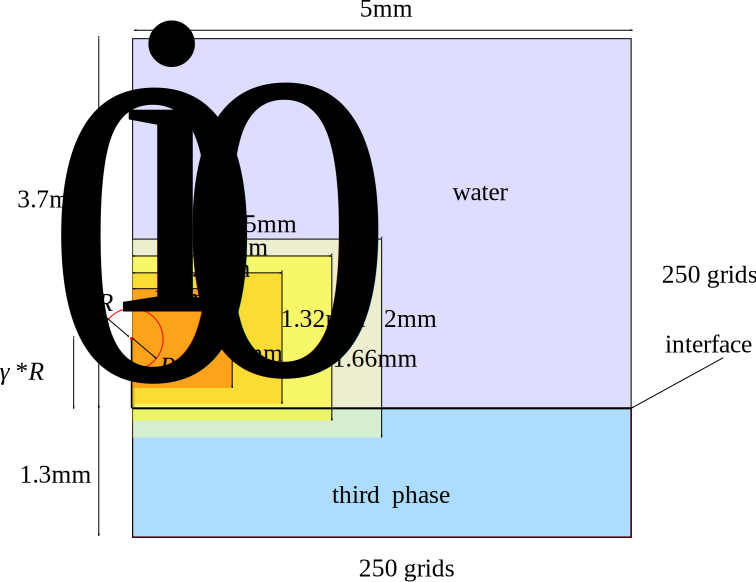
\includegraphics[width=0.7\linewidth]{img/interface.pdf}
    \caption{激光致空泡在软物质界面附近的脉动计算域设置}
    \label{fig:interface}
\end{figure}

软物质界面情景除了物性,使用相同的计算域和计算设置。除了对称轴使用对称边界,旋转面使用wedge边界,其他边界都是“wavetransform”的无反射压力边界,和速度“pressureInletOutletVelocity” 流入流出边界。初始的网格密度为$250\div5mm=50/mm$。经过四次加密,每次加密在选定区域内的$X,Y$方向上数量加倍,也就是区域内一个网格变四个网格。在能够覆盖空泡最大泡半径的区域内,网格密度达到了$800/mm$。不同$\gamma$下的计算域由图\ref{fig:interface}给出。其中空泡的初始半径和最大泡半径使用(12.5$\mu$m-320$\mu$m)这一组合。初始空泡时,半径用10个网格解析。全流场计算域网格数917200。图中的第三相在水气界面案例中为与空泡同物性的气,在水油界面中为硅油。共计算了$\gamma\in \left[0.1:0.1:2\right]$共20组案例。


\subsection{单空泡在水气界面附近的脉动}



\begin{figure}[h]
    \centering
    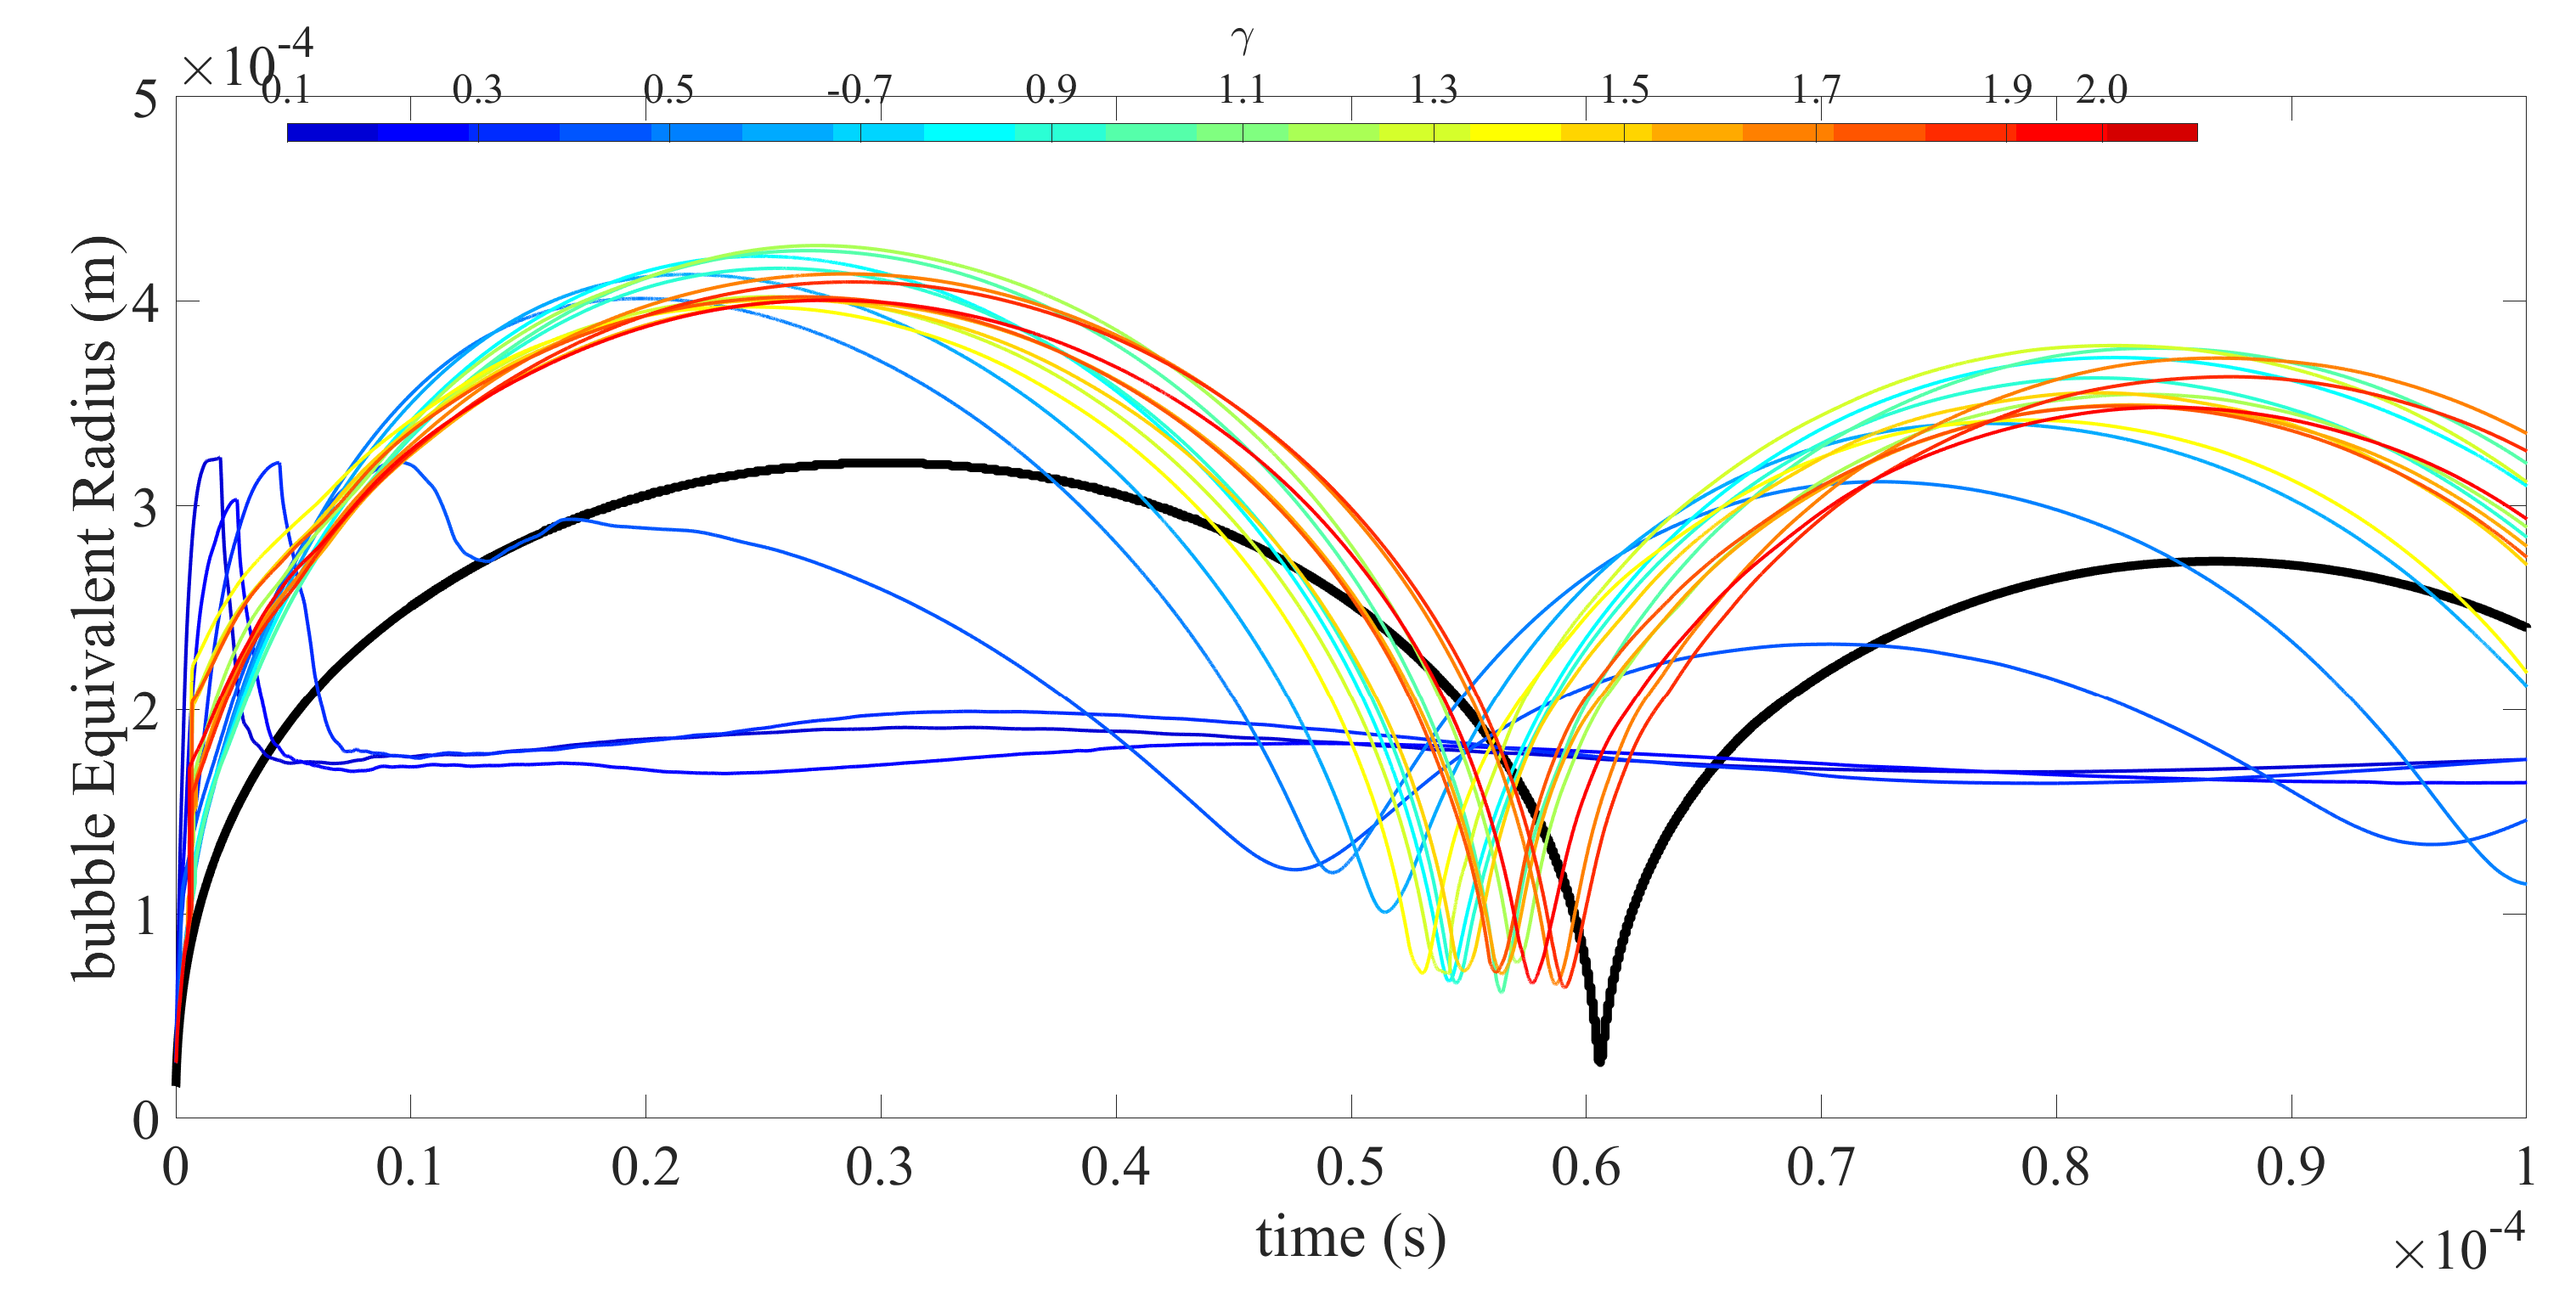
\includegraphics[width=0.9\linewidth]{img/fig3.airradius.eps}
    \caption[空泡距水气界面不同相对距离情形下的泡半径对比图]{空泡距水气界面不同相对距离情形下的泡半径对比图。图中黑色实线为自由域中的模拟结果。}
    \label{fig3.airradius}
\end{figure}

空泡在水气界面附近脉动时,会形成独特的动力学特征,比如双向的射流和王冠形喷溅等。本节中,忽略重力的作用,仅从压强、惯性、张力、粘性和密度等角度考虑空泡在水气界面附近的运动。

图\ref{fig3.airradius}是20组空泡距水气界面不同相对距离情形下的泡半径对比图。图中数据通过模拟计算中每一步记录的空泡体积获得。即$R=\sqrt[3]{\frac{3((360/\alpha)V)}{4\pi}}$。$\alpha$是计算域的张角,前文中有述。
首先发现,空泡在水气界面附近的情况下,最大泡半径获得了提升,而生存周期则获得减小。这是因为在水气界面附近时,空泡推动低密度,低粘的气体相比水更加容易,也就使得惯性驱动的空泡膨胀能够获得更大的半径。

同时可以看到在$\gamma\leq0.3$时,空泡体积等效半径形成的曲线会出小一个暴增,然后急剧减小,随后保持稳定的过程。这是因为空泡距离界面过近形成爆破(burst)效果。爆破指空泡的气体在膨胀过程中,冲破液体表面的阻隔,直接与液面外的气体相联通。在这几个案例中,空泡的气体释放到外界气体中。但因为在模型计算中,将界面气体处理成具有气体物性的第三相,故而仍能追踪其逸出部分在101325Pa下的体积。在其他情景下,空泡半径随$\gamma$增长而减小,其生存周期也逐渐趋同于自由域空泡。

综合考量这20组模拟结果,粗略的将其分为三种情况:A.爆破式($\gamma\leq 0.3$);B.皇冠射流式($0.4\leq\gamma\leq 1.4$);C.突起式$\gamma\geq 1.5$)。因忽略重力作用,实验的分界点与以上的三个值可能稍有不同。


\begin{figure}[h]
    \centering
    \includegraphics[width=0.9\linewidth]{img/fig3.air2.0.png}
    \caption[空泡距水气界面$\gamma=2.0$情形下的相-速度-压力云图]{空泡距水气界面$\gamma=2.0$情形下的相-速度-压力云图。图中白线代表水气界面。界面以上为气,界面以下为水。白线包裹的封闭联通域是空泡。每一帧的右侧是流域的速度场(单位m/s),左侧是压力场(单位Pa)。灰色箭头是速度场的方向。该帧的具体时刻标注在压力场的空白处。以下三个相-速度-压力云图按照同样的标注方式作图。}
    \label{fig3.air2.0pvp}
\end{figure}

图\ref{fig3.air2.0pvp}显示了空泡距水气界面$\gamma=2.0$情形下的相-速度-压力云图。其作为C.突起式$\gamma\geq 1.5$)空泡溃灭的一个典型案例。在这种情景下,空泡的射流情况可以用开尔文脉冲理论解释,即空泡形成远离界面的射流。同时,空泡的膨胀和收缩能够对水气界面形成改造。

第一栏的第一帧显示了该种情况下的计算初始情况,即一个存在于101325Pa的零速度域内的高压初始球形域。随后在第二帧($ 10\mu s$)中,空泡膨胀,在空泡内形成辐射状速度方向。但字啊空泡外的水中,在空泡下壁面,即南极附近,速度矢量仍呈辐射状。但在空泡下壁面以上的位置,水域的速度均最终指向自由界面。这是因为界面以上的气体的密度和粘度均小于水所形成的。值得注意的是,此时因空泡膨胀的推动,此时空泡正上方位置形成突起。第三帧($ 20\mu s$)中,空泡保持膨胀趋势。空泡内部的低压域自由液面以上的气体环境的101325Pa形成明显区别。

第二栏第一帧($ 30\mu s$)附近,空泡到达其最大泡半径,其空泡内部速度降到0,并丧失矢量方向。空泡外的上方形成自空泡始而指向空泡上方的气体区域。下一帧($ 40\mu s$)时,空泡的逐渐收缩。其主要受外界高压的驱动。在速度场中可以看到,与上两帧形成对比的是,速度方向形成了反转。这就在空泡外的上部形成速度自界面开始而指向空泡中心。在空泡外的下方,形成辐射状的指向空泡中心的收缩。在下一帧($ 50\mu s$)中,空泡继续收缩,同时空泡的上表面形成平化现象。相比横向的方向,指向空泡上方方向的速度矢量更多,同样也强于均匀的辐射收缩的下方。

在第三栏第一帧($ 55\mu s$)中,速度流延续了上文中的趋势,继续密集的指向了空泡上方位置。而因这种挤压在空泡的上方位置形成一个高压区域。这个高压区域将驱动空泡上方位置的水体继续加速的向空泡内部流动,即驱动形成射流,也成为支撑界面突起的一个因素。在下一帧($ 59\mu s$)中,自空泡上方射入的射流击穿空泡并撞击空泡下壁面。如此,形成撞击的高压。此时场内的速度仍如同上一帧一般的指向空泡的中心位置。在最后一帧($80 \mu s$)中,空泡中的击穿射流仍然存在,但同时空泡已经开始进入第二个生命周期。后续将在其新位置继续脉动。

本例中,空泡离界面位置较远,其形成的相互作用效果不明显。但其射流方向与使用开尔文脉理论(见章节\ref{chapter1.2.2.2})的参数$\bm\zeta=+0.195 \gamma^{-2} \bm n $计算获得的$\bm\zeta$预言的矢量方向和射流强度相一致。同时,自由界面并没有形成鲜明的变化,而只是因为空泡膨胀和空泡的不均匀收缩形成轻微的突起。

\vfill



\begin{figure}[h]
    \centering
    \includegraphics[width=0.9\linewidth]{img/fig3.air0.7.png}
    \caption{空泡距水气界面$\gamma=0.7$情形下的相-速度-压力云图}
    \label{fig3.air0.7pvp}
\end{figure}

图\ref{fig3.air0.7pvp}显示了空泡距水气界面$\gamma=0.7$情形下的相-速度-压力云图。该情景下形成了一种特殊的射流方式,即皇冠(crown)射流。其通常发生在空泡膨胀期,并形成于收缩过程中。本例作为B.皇冠射流式($0.4\leq\gamma\leq 1.4$)的一个典型案例解释该类型空泡脉动过程中的动力学现象。

在第一栏中,第一帧仍是空泡的初始状态。第二帧($10 \mu s$)中,空泡膨胀形成一个卵形壁面形状。这是空泡近界面处的水的质量更小,外界气体密度和粘度更小导致的。这就使得空泡在靠近界面处的反向延展。同时,可以看到,空泡推动水体形成近辐射状速度。在空泡的下方(南极)附近形成相比$\gamma=2.0$情况下更窄范围的辐射状流速度。在这个范围以上形成弯曲的指向自由面的速度,并在界面处形成速度突变。而在空泡的上方由于推动效果,水体的速度更快。在下一帧($20\mu s$)中,由于速度指向自由面,在空泡的水平中轴以上部分的空泡壁面推动水体想空泡上方那个汇集,于是在空泡的正上方位置形成局部高压。这个高压将推动汇集到空泡正上方的水体向上和下两个方向运动,也就是射流的形成。在第四帧($25 \mu s$)中,自空泡中轴以上向空泡上方汇集的速度仍然存在,自空泡下方指向自由面的速度也仍然存在。因这种汇集作用继续推动,空泡上方的高压区域继续加强和扩展。同时也在自由面附近的位置也就是空泡壁面横向最大处的上方形成一个突起,这个突起将在后续形成皇冠式喷溅。而高压区域继续推动深入自由气体域和指向空泡的射流继续运动。

在第二栏第一帧($ 35\mu s$)中,空泡开始收缩,空泡外流场内的速度矢量出现方向反转。但在射向气体域的射流中,高压区域以上,速度矢量仍旧保持向上,也就是射流仍向上延展。高压区域同时仍旧推动射入空泡内部的射流继续运动。但注意到,因自由面处形成突起,其在收缩时处于落后状态,继而会在此处形成所谓的皇冠喷溅。在下一帧($ 40\mu s$)中,空泡继续收缩,双向射流在高压区域的推动下继续运动。而高压区域的的高压最值近从2.1$\times10^5$Pa下降到了1.9$\times10^5$Pa。此时空泡上方的速度进入到空泡内部,并知道靠近下壁面的位置减速为零。而因这个自上而下的速度的限制,自其他方向进入空泡的速度,也在壁面附近减速为零。在下一帧($45 \mu s$)中,射流到达空泡下壁面。注意因空泡在溃灭后期形成的高速度,也就是在内外压强差的驱动下,水体向空泡内的汇聚速度持续加快,从而形成空泡上方的射流源处压力再次增强。由此推动射流的继续加速。在该栏第四帧中,向下的射流击穿空泡向上的射流继续向上运动。而空泡形成被射流击穿的双层结构。

在第三栏第一帧($ 55\mu s$)中,空泡发生溃灭后的小空泡多次溃灭。其辐射的冲击波对场内速度指向形成改造。可见图中杂乱的速度方向。在图中未显示到的,在计算域内可见多层的速度方向的突变。注意到此时的皇冠射流随速度指向已经运动到更靠近向上射流的位置。在第二($ 60\mu s$)、第三($ 70\mu s$)和最后一帧($ 80\mu s$)中,空泡再次形成膨胀和收缩过程,此时又形成新的皇冠射流,形成多层的类似树叉型的射流状态。

在本例中,空泡距离自由面的距离较近,其机制以膨胀形成双向射流和收缩时形成皇冠射流为特征。这种情况下,空泡与界面的相互作用更加激烈,空泡对界面形成明显的外形改造,而界面则为空泡的射流加速,即所谓的弹弓效应。




\begin{figure}[h]
    \centering
    \includegraphics[width=0.9\linewidth]{img/fig3.air0.2.png}
    \caption{空泡距水气界面$\gamma=0.2$情形下的相-速度-压力云图}
    \label{fig3.air0.2pvp}
\end{figure}


图\ref{fig3.air0.2pvp}显示了空泡距水气界面$\gamma=2.0$情形下的相-速度-压力云图。其作为A.爆破式($\gamma\leq 0.3$)空泡与界面的相互作用的典型代表在此处给出其形态学和动力学过程。

图中第一栏第一帧是空泡的初始状态。第二帧($ 1\mu s$)中,空泡膨胀,但因距离界面过近,空泡与自由气体的之间的水体过薄,在推动空泡外水体运动时,形成的拉伸效果将该水体拉断,从而形成图中的爆破效果。因密度和粘度的限制,空泡主要的能量释放方向是近自由面。远自由面方向空泡壁面的运动主要由惯性驱动。从图中速度图可以看到,在爆破形成时,空泡内的气体向自由气体域高速运动。其速度在本帧时刻仍在100m/s数量级,远高于空泡内其他位置的气体。空泡内气体释放到自由气体中后,空泡内外压强行成一次再平衡,这也补充了空泡重生再膨胀的能量。
空泡爆破形成的水尖刺,因空泡气体的推动和空泡推动液体形成的挤压而持续向上运动,形成类似射流的效果。同时可以看到空泡在形成初期辐射的冲击波。因本算法的初始设置更加物理,其对空泡与冲击波的伴生现象相对更加物理,可以用来解释冲击波衰减后的现象,此处不详述。空泡推动形成的辐射状速度场矢量方向,在除空泡下方南极附近辐射指向外,其他方向因冲击波的改造形成指向壁面。
在下一帧($ 8\mu s$)中,空泡的爆破效果愈发明显。自空泡向自由气体域喷射的气体仍高速向竖直上方运动,同时也在横向的推动其本地气体运动。同时水尖刺也在向上延展,并且有横向的向对称轴运动的趋势。空泡横向中心轴以上的位置的速度继续挤压这个水尖刺,促使其继续运动。空泡内部没有形成如上两例中直到低压极限的表现,而是高达一半的大气压,这是与自由气体连通的效果。图中红色高速区域即外界气体进入空泡内部的表现。
在第四帧($ 16\mu s$)中,上述的尖刺结构横向运动后撞击,并形成向上和向下的射流的物质释放通道。此时场内的速度矢量仍多数指向自由面。空泡在水体内的膨胀,使得空泡横向中心轴以上部分仍挤压这个尖刺结构。同时可以看到,进入空泡内部的自由域气体在空泡内部形成特殊的高速读结构,其会冲击空泡壁面,造成一定的形变。此时空泡内的气体再次封闭,形成卵状结构。

在第二栏第一帧($20 \mu s$)中,空泡封闭后形成的双向射流继续向双方向发展。而封闭的尖刺结构因空泡推动和后续速度的挤压,在空泡正上方,也就是碰撞区域形成一个高压点。这个高压区域将继续推动双向射流的发展。而因为空泡的封闭,外来气体的速度撞击,以及水体惯性运动形成的空泡的继续膨胀,空泡内部压强减小,形成空泡的收缩趋势。因密度和粘度的问题,空泡在压强差驱动下的收缩仍最先发生在近自由面,也就是空泡的上方壁面最先开始收缩,即本栏第二帧($25 \mu s$)。此时的空泡下部仍在继续膨胀,空泡上方因压差形成尖刺结构的内凹,并由此将射流分裂出类似皇冠射流的结构,上射流形成多层结构。射流根部空泡上部的高压将推动空泡和射流形状的继续演化,即下一帧($40 \mu s$)中,上射流形成类似竖叉式结构,而下射流继续向射流相对壁面运动。而此时空泡上方的水层因空泡的收缩和速度的汇集,以及再次加厚,成为水射流稳定的物质来源。最后一帧($45 \mu s$)中,下射流击穿空泡,使空泡产生凸起结构,为接下来的双层空泡结构奠定基础。

在第三栏($ 50\mu s$,$60 \mu s$,$70 \mu s$,$ 80\mu s$)中,主要展示了远离自由面,指向空泡内部的水射流贯穿空泡的动力学过程。因射流的高速运动,射流裹带空泡气体向下方向运动,形成了特殊的双层空泡结构。即空泡部分在原位置,一部分突破的空泡位置的下方。在这个过程中空泡的泡内气体的物质量充足,没有发生溃灭现象。而且,射流在这个过程中因后续速度的继续挤压,仍旧向上延展和变形。注意,在实际中,因重力的作用,上射流会更早地进入回退进程,此处不讨论。

在本例中,空泡与自由气体之间的水体层过薄,在膨胀初期即破裂,由此形成这种空泡的爆破机制。空泡膨胀时推动液体向其上部运动,形成尖刺结构,这种结构在后续水体的推动下相互碰撞,继而产生上下两股射流。因空泡破裂与外界压强发生平衡,所以空泡最后没有形成溃灭现象,而是被射流推动形成多层结构。


\begin{figure}[h]
    \centering
    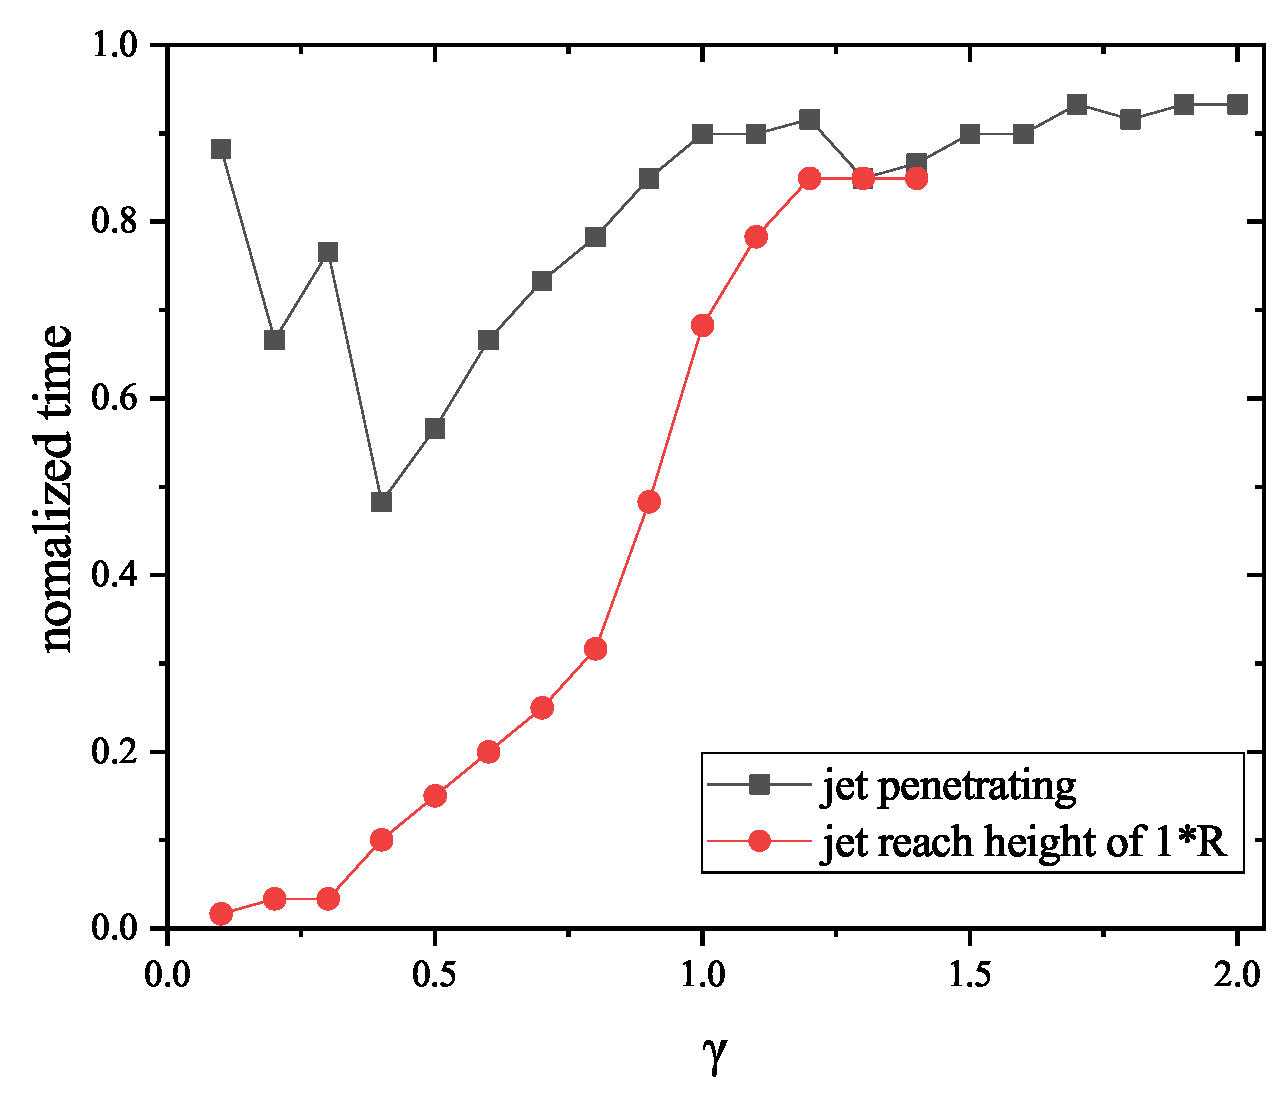
\includegraphics[width=0.6\linewidth]{img/fig3.airjettime.eps}
    \caption[水气界面附近情景下射流击穿时间和上射流到达一倍半径的归一化时间]{空泡距水气界面不同相对距离情形下的下射流击穿时间和上射流到达一倍半径距离的归一化时间。黑色是射流击穿时间,红色是上射流到达一杯空泡半径距离时间。}
    \label{fig3.airjettime}
\end{figure}

在共20组结果中,每组都发生了非对称的溃灭现象,即射流。为了对空泡与自由面的相互作用和射流的强度进行某种量化,将指向空泡内部的射流到达对立壁面的时间作统一的归一化处理,即$T_\mathrm{nomalizd penetrating}=t_\mathrm{penetrating}/t_\mathrm{freeosc}$。其中$t_\mathrm{penetrating}$指空泡射流到达对立面的时间, $t_\mathrm{penetrating}$指上文中空泡在自由域的体积最小时间。同时我们对上射流的更关注其形成后的速度,也定义了一个能间接反应其速度的归一化时间,$T_\mathrm{nomalizd-jet-reach}=t_\mathrm{jet-reach}/t_\mathrm{freeosc}$。其中$t_\mathrm{jet-reach}$指空泡的上射流到达1倍自由域内空泡最大泡半径$R=330mm $的时间。

从图\ref{fig3.airjettime}中可以看到,下射流的击穿空泡时间在$\gamma \geq 0.4$范围中,是随着$\gamma $的增长而变晚的。在$\gamma \leq 0.3$中因形成了爆破式相互作用,其射流形成机制与其他情形不同,故而较晚。但整个过程中形成的上射流,即指向自由气体域的射流到达一倍R的时间是越来越晚的,就表明上射流的初始速度是随着空泡与界面距离的增加而减弱的。因$\gamma \geq 1.5$没有形成向上的水射流,而仅是凸起形态,此处不涉及。


\begin{figure}[h]
    \centering
    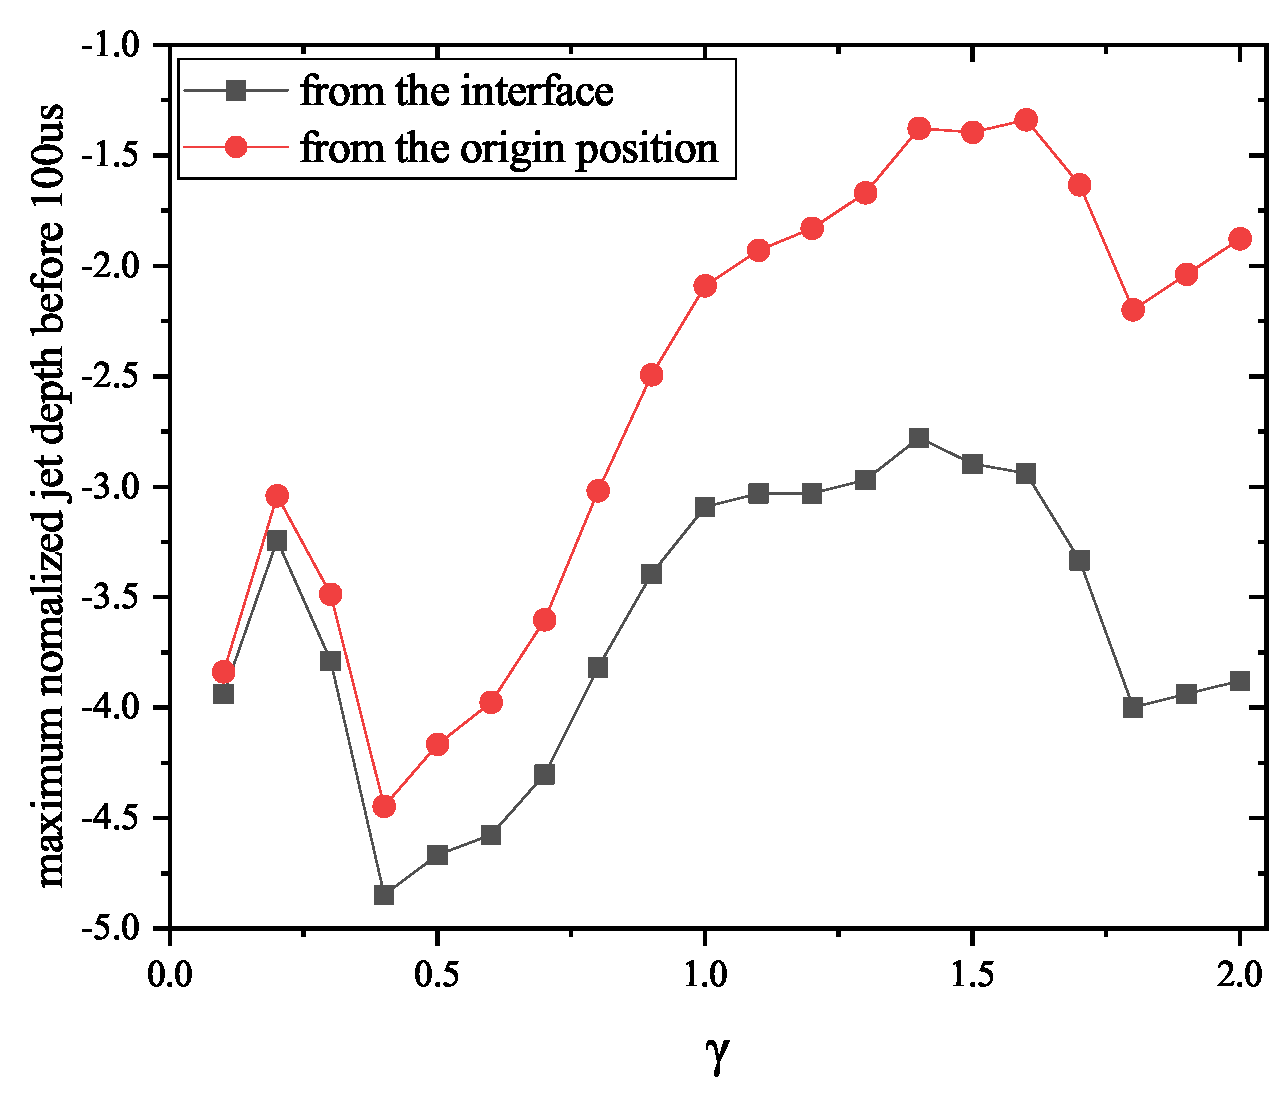
\includegraphics[width=0.6\linewidth]{img/fig3.airdistance.eps}
    \caption[空泡距水气界面不同相对距离情形下的归一化射流深度]{空泡距水气界面不同相对距离情形下的归一化射流深度。黑线是以界面为基准,测量的深度。红色是以空泡初始位置为基准形成的深度。负值表示深度。}
    \label{fig3.airdistance}
\end{figure}

向下的射流,即击穿空泡的射流,在水中受到水的阻滞,其传播距离有限。通常在较长时间范围内,通过空泡的多次脉动,其可以达到十几倍R的距离。此处我们只关注其在第一个生命周期结束后直到第二次生命周期结束前的$100\mu s $内传播的最远距离。从图\ref{fig3.airdistance}中,我们可以看到,在B.皇冠射流式($0.4\leq\gamma\leq 1.4$)相互作用范围内,空泡的射流深度是随着$\gamma $的增加而变浅的,反映了自由面对空泡的弹弓效应是随着自由面与空泡初始位置的距离变大而减弱的。在C.突起式$\gamma\geq 1.5$)相互作用范围内,其存在一个过渡的区域和一个彻底的凸起式的区域,但其深度确实在一定范围内比某些情况深。而在A.爆破式($\gamma\leq 0.3$)范围内,因涉及到压力再平衡,其溃灭烈度远小于未连通的其他两种情况,从而其射流深度也小于B的某些情况。









\subsection{单空泡在水油界面附近的脉动}
硅油是一种稳定无毒的有机油类。其在工业上应用广泛。特别的,通常因其可调节粘度,而作为一种研究空泡受粘度影响的环境液体。本文选取一种实验室易获得的硅油($\mathrm{C_2H_6OSi}$)作为液-液界面情况的第三相,见图\ref{fig:interface}。
这种硅油的具体性质已在在上文中给出(表\ref{tab:3.1})。其本身的实际物理参数表现为一种高粘性液体。如果要针对某一个具体的特性研究其对空泡的影响,可以设置实际实验上难以获得的物性参数。但此处仍选择其真实物理性质。

通常激光空泡的环境液体因为粘性增加,会加剧了空泡脉动的能量耗损,从而造成空泡脉动现象的减弱,包括生存周期变小和射流现象的减弱。而高粘液体作为流域的一部分,也会对空泡造成相似的影响。因兼具可流动和高粘度的边界特性,水油界面附近水体内产生的空泡,会表现出兼具自由界面和固体界面附近的特性。

\begin{figure}[h]
    \centering
    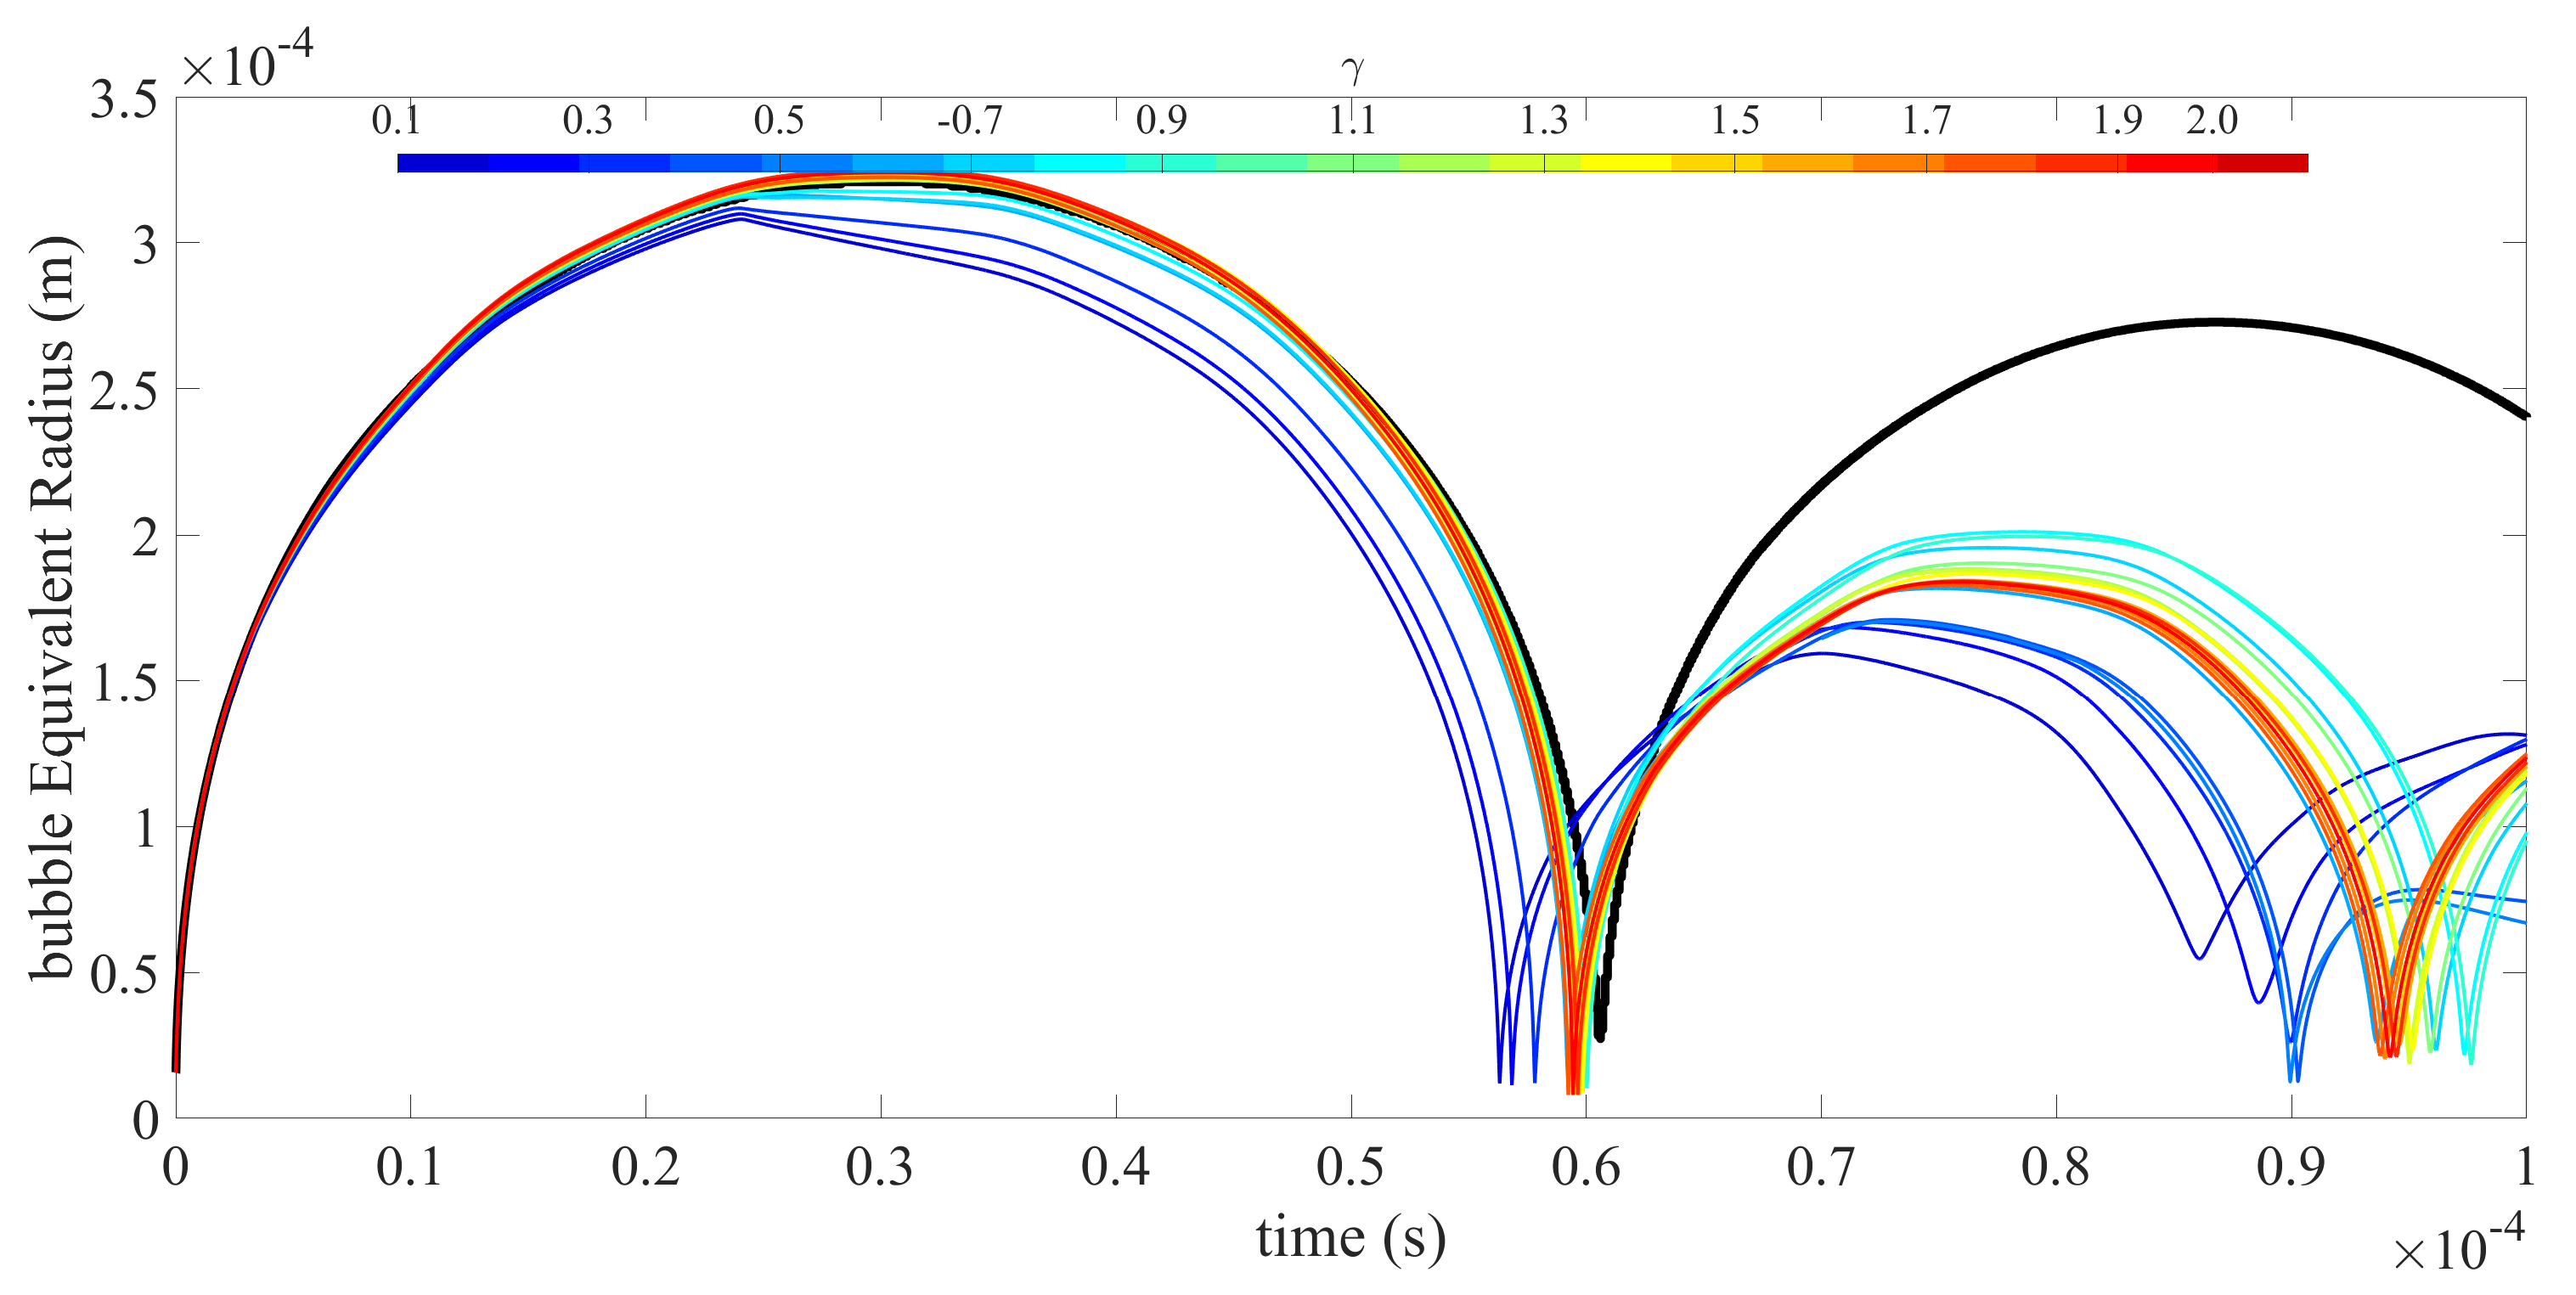
\includegraphics[width=1\linewidth]{img/fig3.oilradius.eps}
    \caption[空泡距水-硅油界面不同相对距离情形下的泡半径对比图]{空泡距水-硅油界面不同相对距离情形下的泡半径对比图,图中黑色实线为自由域中的模拟结果。}
    \label{fig3.oilradius}
\end{figure}

\begin{figure}[H]
    \centering
    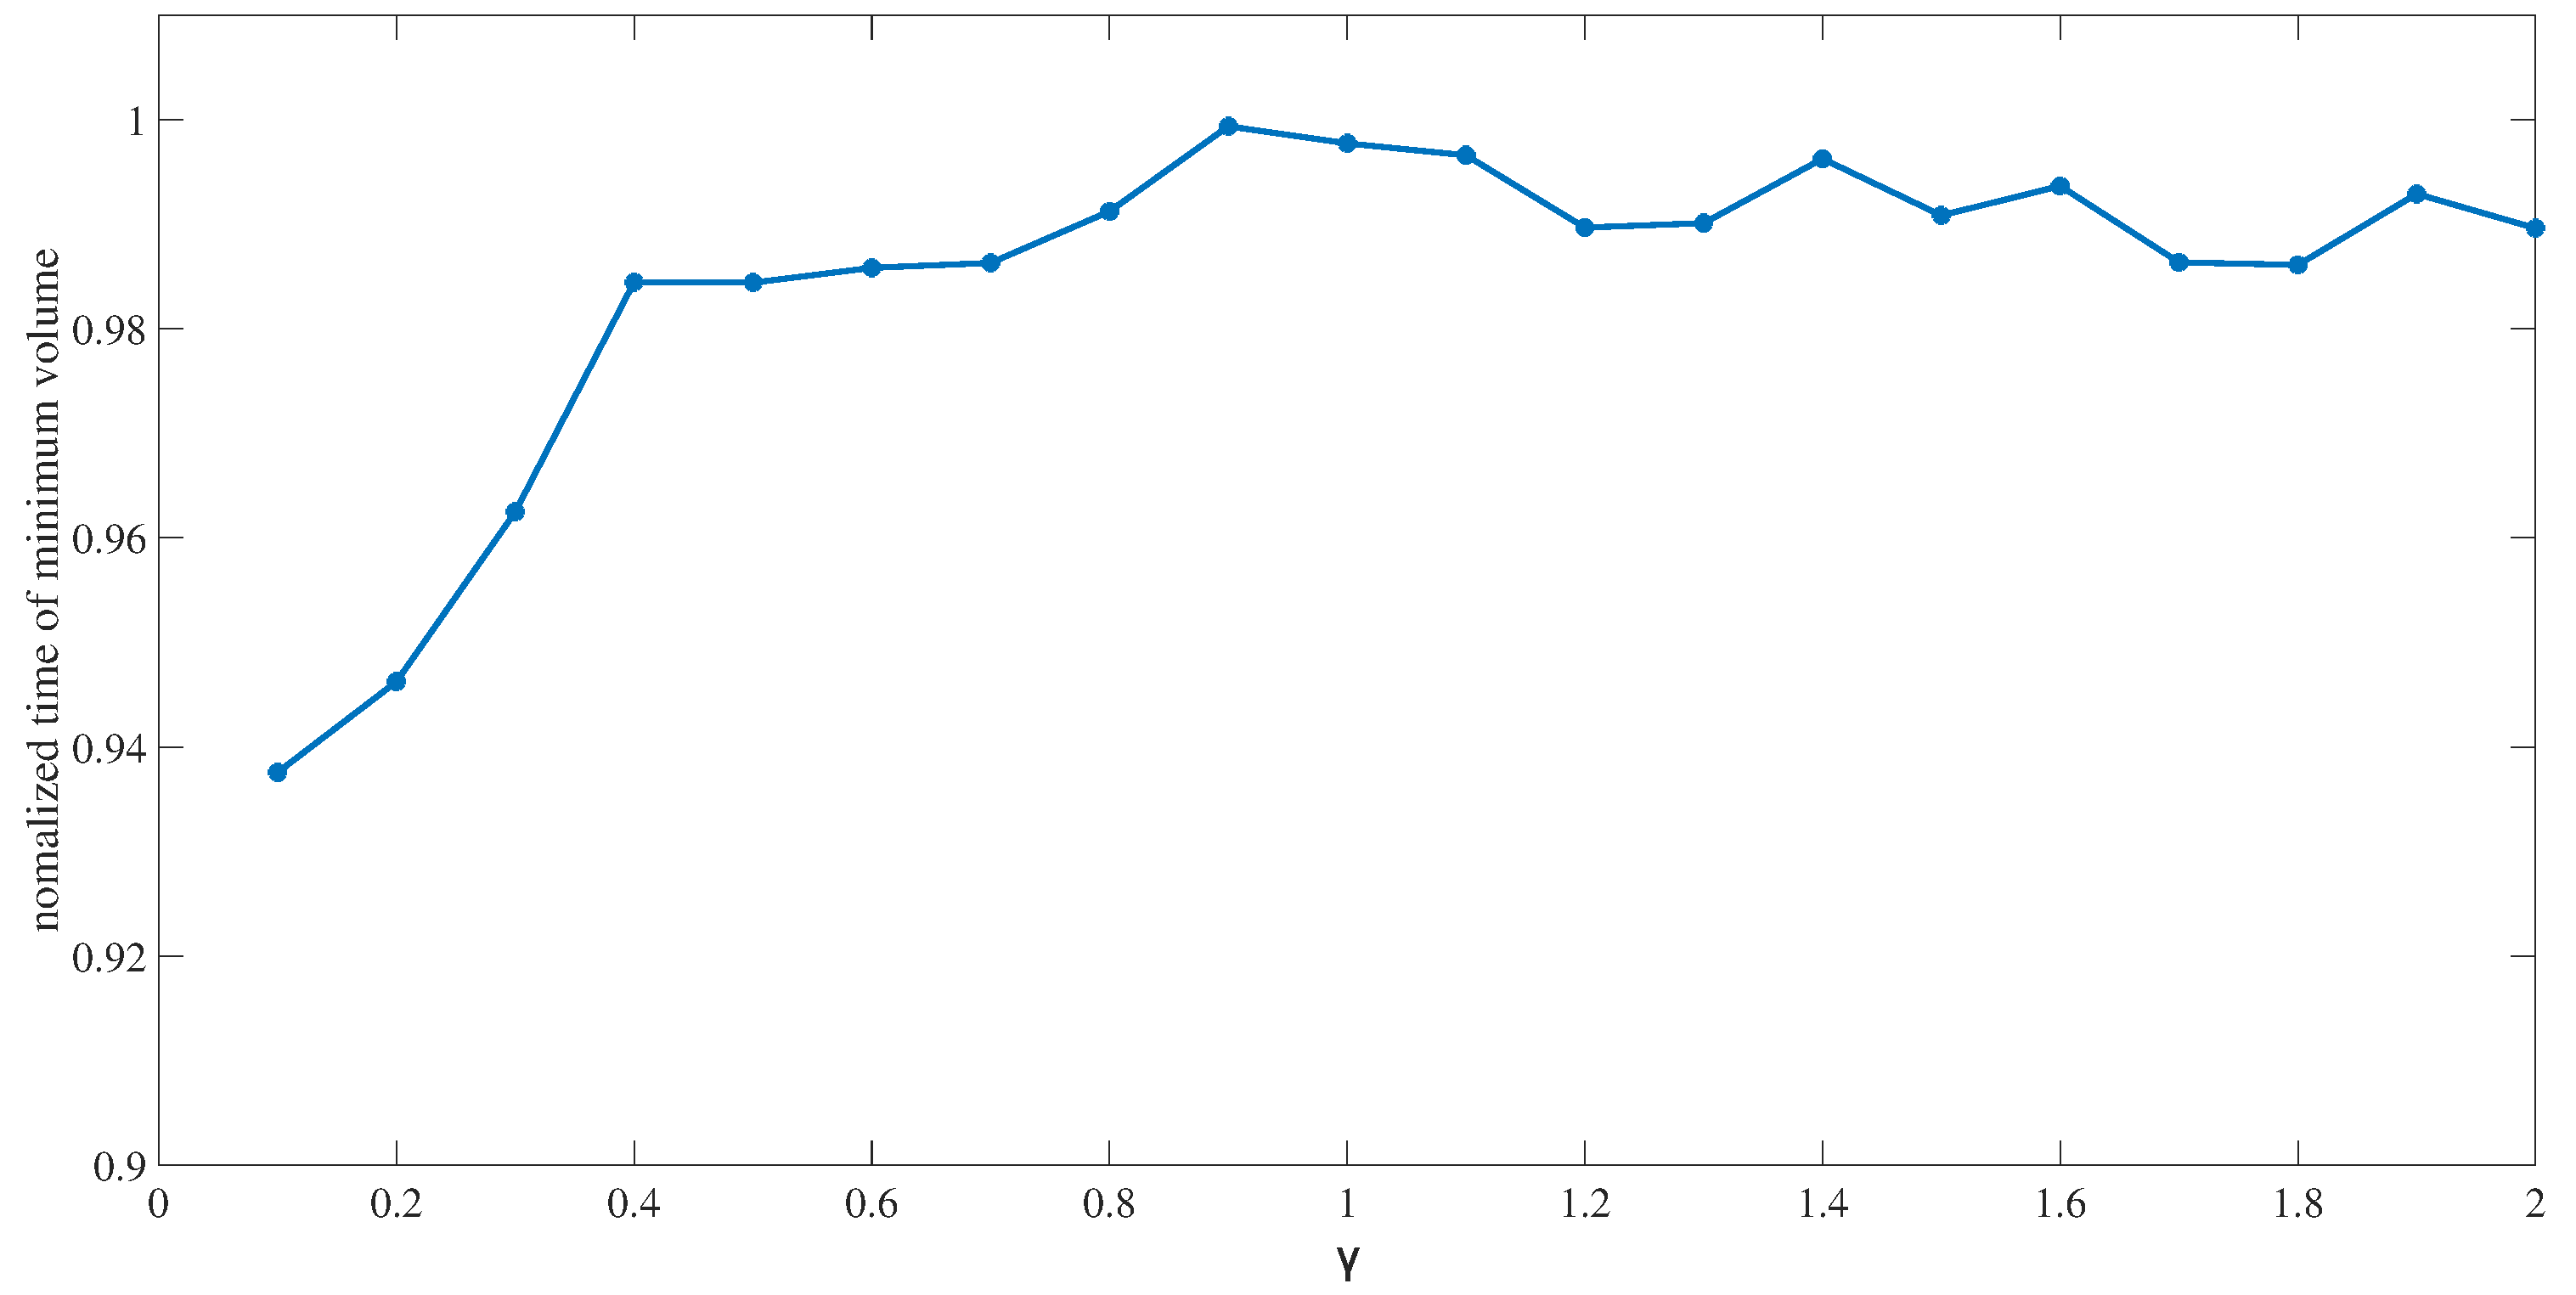
\includegraphics[width=0.9\linewidth]{img/oilclpstime.eps}
    \caption[水-油界面附近空泡的归一化溃灭时间]{水-油界面附近空泡的归一化溃灭时间。归一化时间通过模拟计算中获得的体积最小时间除以自由域中的体积最小时间60.06$\mu s $获得。}
    \label{fig:oilcolltime}
\end{figure}

图\ref{fig3.oilradius}中给出了空泡与水油界面在不同相对距离$\gamma$处的体积等效半径对比图。可以看到,在$\gamma$越大,也就是越接近自由的情况下,空泡的体积等效半径越接近在自由域中的脉动。
在$\gamma\leq 0.3$,也就是空泡在界面附近时,空泡的半径在膨胀到最大泡半径之前,大约$24\,\mu s$左右开始出现明显地受压迫而减缓增长加速溃灭的现象。这是因为由于与界面距离过近,膨胀过程中推动密度高,粘性高的硅油而耗费能量,并因张力影响而提前回弹。从图\ref{fig:oilcolltime}中通过归一化放大溃灭时间的差异后,可以看到空泡的生存时间形成明显的阶段性区分。$\gamma\leq 0.3$ 时,溃灭时间形成一个明显的上升趋势。$\gamma$其脉动时间越接近自由脉动。
$0.4\leq\gamma\leq 0.6$时,溃灭时间形成一个平台。
$\gamma\geq 0.7$时,溃灭时间形成一个波动曲线。这三个阶段的体积等效半径的变化对应了不同的空泡脉动形式。通过对其场内各向异性的性质研究,我们可以获得更细致的信息。



从空泡自身溃灭形式的角度区分,空泡总体上可以分为两种溃灭模式,断裂式($\gamma\leq 0.6$)和射流式($\gamma\geq 0.7$)。断裂式指空泡溃灭时,横向的受到冲击,从而形成接近界面和远离界面的两部分。射流式指空泡在溃灭后期纵向的形成射流的趋势,并在随后的回弹中表现出强射流的溃灭。其中断裂式又可以细分为:A.断裂接触式($\gamma\leq 0.3$)和B.断裂射流式($0.4\leq\gamma\leq 0.6$)。A.断裂接触式指空泡在溃灭时,其横向的冲击在空泡内部没有形成纵向的击穿空泡的射流,而是以空泡贴近界面的方式影响界面。而B.断裂射流式指空泡在横向断裂时,同时产生了射向界面的射流了,并击穿空泡射向界面。
下文中将结合三种情况的典型案例($\gamma= 0.1$,$\gamma= 0.5$,$\gamma= 2.0$)的相-速度-压力图详细地解释几种机制的动力学过程。


\begin{figure}[h]
    \centering
    \includegraphics[width=0.9\linewidth]{img/fig3.oil.2.0.png}
    \caption[空泡距水-硅油界面$\gamma = 2.0$情形下的相-速度-压力云图]{空泡距水-硅油界面$\gamma = 2.0$情形下的相-速度-压力云图。图中黄线代表水油界面。界面以上为油,界面以下为水。每一帧的左侧是流域的速度场(单位m/s),右侧是压力场(单位Pa)。白色线表示气体空泡的轮廓。黑色箭头是速度场的方向。该帧的具体时刻标注在压力场的空白处。以下三个相-速度-压力云图按照同样的标注方式作图。}
    \label{fig3.oil2.0}
\end{figure}

图\ref{fig3.oil2.0}显示了空泡距水-硅油界面$\gamma = 2.0$情形下的相-速度-压力云图。第一帧表示该情景下的初始状态,即0时刻。第二帧($10\mu s$)中,显示了空泡的初始膨胀阶段。此时空泡壁面在向外急剧的扩张,速度仍近100m/s,场内的速度矢量自空泡初始位置呈放射状发展。这是由于空泡在初始时刻向外释放的冲击波几何传播,推动当地液体实现的。而由于空泡膨胀超出了其均衡半径,此时其泡内压降到了环境压以下。在膨胀一段时间后,空泡在$31\mu s$左右达到最大泡半径。可以看到第三帧中空泡外已经形成指向空泡内运动的速度。而空泡内部与自由域的最大泡半径时空泡各向同的向内收缩不同,此时空泡受界面影响形成局部的压力梯度,空泡内部形成自远离界面到靠近壁面方向的速度。速度的终点在靠近空泡上壁面附近。这也为射流的形成埋下伏笔。

在第二栏中,显示了空泡收缩的过程。其中第一帧($45\mu s$)中上述的速度终点区域向泡中心移动,稍微远离了空泡壁面。空泡壁面的速度达到了约8m/s。在下一帧($57\mu s$)中速度终点的位置持续向中心移动,但仍处于空泡内部的上方位置。全流域受泡外压的驱动向空泡运动,同时因速度提升和几何限制的原因,空泡壁外的压力受到一定的提升,并作用于速度的继续提升。而这时,空泡壁面速度已经达到30m/s以上。随后在第三帧($59\mu s$)中,约两微秒的时间,空泡壁面的速度已经达到了120m/s。而上述的压力提升在空泡的下方,也就是远离水油界面的位置,产生了更高的压强。这为空泡自空泡下方形成向上的射流提供了必要条件。

第三栏中,就显示了空泡的射流击穿,及其后续的再膨胀过程。第一帧($60\mu s$)中,空泡非球型溃灭,空泡向外辐射了一个冲击波。而其因非球型溃灭形成的击穿射流,此时也击穿空泡近界面的壁面。这个射流的速度在180m/s左右。辐射的冲击波在界面处发生了透射和发射。在射流击穿后($64\mu s$)继续向界面移动并持续减速,空泡继续膨胀。在第($77\mu s$)图像中显示,射流裹带的气体因速度减小,以及表面张力和空泡收缩的共同作用,被留在原地成为一个独立的小空泡。而大空泡将继续其脉动生命周期。

在本例中,空泡的脉动表现出接近自由域的脉动性质,同时也产生了受液面影响的射流。这与使用章节\ref{chapter1.2.2.2}中
$\bm\zeta=0.195 \gamma^{-2}\left(\rho_{1}-\rho_{2}\right)\left(\rho_{1}+\rho_{2}\right)^{-1} \boldsymbol{n}$计算获得的$\bm\zeta$预言的矢量方向和射流强度相一致。




\begin{figure}[h]
    \centering
    \includegraphics[width=0.9\linewidth]{img/fig3.oil.0.5.png}
    \caption{空泡距水-硅油界面$\gamma = 0.5$情形下的相-速度-压力云图}
    \label{fig3.oil0.5}
\end{figure}

图\ref{fig3.oil0.5}显示了空泡距水-硅油界面$\gamma = 0.5$情形下的相-速度-压力云图。
第一栏第一帧显示了空泡的初始状态。第二帧($ 15\mu s$)显示空泡的初始膨胀阶段。在这帧中,空泡向外辐射状的膨胀。在壁面到达界面附近时,推动界面变形。因硅油更重更粘,其流动较水的流动变化更满,速度更慢。从而使空泡更倾向于在远离界面方向释放空泡能量。也就是在空泡远离界面的壁面的速度相较与界面相对的壁面速度更快。因泡内低压少物质的特点,泡内的速度中心也就是零速度点,约等于空泡南北极速度的中心点,位置向上移动到靠近壁面处。在第三帧($ 25\mu s$)中,空泡远离界面的下壁面因水的惯性仍在向外膨胀中。而界面附近处的上壁面因其速度一直慢于下壁面,而且界面因张力而倾向于恢复其初始状态,使上壁面相比下壁面更早的进入到收缩周期。此处就对应着图\ref{fig3.oilradius}中的转折部分。进而空泡形成自界面向水体内的速度。

在第二栏中,($30\mu s$)帧显示了空泡下壁面膨胀到最大的情景。上壁面持续向内收缩,下壁面内的气体有向外膨胀的速度,但泡外的水已经开始进入回归进程。下一帧($ 53\mu s$)中,空泡持续收缩,并且在靠近界面的上壁面发生平化现象。而界面则将空泡膨胀形成的挤压和拉伸以剪切波的形式传播了出去,形成了界面特殊的形变。而此时,空泡的速度终点位置已经回到空泡的初始位置附近。特别的,我们可以注意到,在空泡水平轴以上和平化壁面以下位置,形成一片高速度区域。这片高速度区域是在界面回弹的基础上叠加收缩形成的。在($ 58\mu s$)时其非常明显的形成一个向内凹陷的区域。因为其对应着速度终点的位置,域内的流体物质向速度终点汇集,继而引发该位置的高压和高速度。而高压高速度将变成壁面的驱动力,以完成下一栏的动力学表现。

第三栏中,第一帧($ 59\mu s$)表示了上栏第三帧的下一微秒的状态。此时空泡,因高压高速区域驱动壁面运动,继而撞击,形成水锤辐射高压并将空泡自撞击位置切断。水锤压在弯曲界面处发生复杂的反射和投射,形成特殊的压力场。而因为撞击前特殊的空泡形状,撞击后形成特殊形状的水射流,即在靠近壁面的部分中形成单束水射流,而在远离界面的部分中形成辐射状的圆锥射流。从而使上部分的残留空泡内形成单射流撞击。在下部分残留空泡形成特殊而花托状。下一帧($ 60\mu s$)则更加清晰,单射流击穿上部分空泡,并对界面造成尖刺状形变。而空泡也随着射流向界面运动,形成心形$\spadesuit$射流。下部分空泡则明显的形成了一种圆锥状溅射。在最后一帧$ 70\mu s$)中,射流裹带空泡气体向界面运动到失去速度,而因空泡膨胀射流失去后续水射流的填充,继而在空泡内发生断裂,成小液滴。而下部空泡的膨胀也挤压使圆锥状射流合并和脱落。

这种情况下,空泡膨胀时会推动水油界面移动和变形,油体会对空泡壁面移动进行减速和推动空泡重心位置变动。在空泡收缩时,界面同样使空泡壁面发生变形,从而形成特殊的撞击溃灭结构,进而使空泡横向的撞击溃灭,分裂成两部分,其中靠近界面的一部分被射流击穿,进而射流推动界面运动。

\begin{figure}[h]
    \centering
    \includegraphics[width=0.9\linewidth]{img/fig3.oil.0.1.png}
    \caption{空泡距水-硅油界面$\gamma = 0.1$情形下的相-速度-压力云图}
    \label{fig3.oil0.1}
\end{figure}

图\ref{fig3.oil0.1}显示了空泡距水-硅油界面$\gamma = 0.1$情形下的相-速度-压力云图。这种情况下,空泡和界面发生最强烈的相互作用。该图第一帧仍是初始状态。第二帧($10\mu s$)中,空泡辐射式膨胀,但空泡膨胀使上壁面在更早期直接接触水油界面。空泡的膨胀受界面的明显约束,从而空泡的下壁面运动速度快于与界面相接触的上壁面。于是形成空泡近界面的部分平均半径小于其下半部分。这样就使空泡的速度零点的位置更靠上,甚至超过空泡初始位置。在第三帧($25\mu s$)中,空泡的速度零点明显上移到原界面位置之上。此时其处于最大泡半径时刻,远离界面的壁面仍在向外低速膨胀,而近界面的上壁面已经开始收缩。此时对应图\ref{fig3.oilradius}中的明显转折。而可以注意到,在界面-水体-空泡的交接处,此时形成速度高区,这也使后续此处发生特殊的形变。而因上下不均衡的膨胀,使此时空泡下方的半径超过自由域的最大泡半径。

随后在收缩阶段的第二栏第一帧($43\mu s$)中,空泡收缩时其速度零点,或者速度终点在空泡的下半部分。这是空泡近界面的上壁面的收缩早,速度快导致的。而因为这个速度终点的位置低于中间形成的突起部分,使得突起上下的壁面保持这种相位领先直到空泡溃灭。于是产生下一帧中($56\mu s$)空泡上下两个凹陷。而此时空泡的收缩使界面回弹到近初始位置,也对界面造成形变。值得注意的是,此帧中空泡的下半部分因形成凹陷结构,这种结构的收缩形成水体的撞击,从而形成辐射冲击波。这种冲击波有加速了空泡的溃灭过程。因形成了两个凹陷结构,在($57\mu s$)中,空泡的溃灭形成两处断裂。这点可以从空泡分裂成三个大部分看出。其中上、中两个大部分中间形成了一个锥形射流隔断中,从而使上部分形成一个环形空泡。而中间部分,则被自下而上的环形射流击穿,并向上突入环形空泡内部,推动界面变形。而下部分,则因凹陷的撞击和下突起的运动,也被截断成两部分。一部分随圆锥射流进入中大部分空泡内部,下半部分被射流裹带向远离界面的方向运动。

随着空泡的继续脉动,在($58\mu s$)也就是第三栏第一帧中,上中两个大部分合并成一个新的大空泡,直接接触界面并继续膨胀。而下大部分由于分成了两部分,其进入大空泡内部的一部分因射流的断裂而与大空泡融合,并接续的向外膨胀。另外部分则逐渐结合在一起形成了新的空泡。于是如第二帧($66\mu s$)中,空泡重新组合成两个大空泡,其中的主体部分大空泡与壁面接触而继续膨胀,并且其中深入的到另一个空泡的尾巴持续收缩。而另一个空泡则膨胀,一挤压尾巴回归,二挤压尾巴断裂部分的向外加速。在最后一帧($70\mu s$)中,主体空泡开始收缩,另一个空泡被动变形。

在本例中,空泡初始位置极为靠近界面,导致其动力学受硅油影响较大。其膨胀和收缩均受到限制,从而形成特殊的溃灭形态,在横向壁面撞击后,空泡被割裂成几个有关系的个体。

在以上三种情况中,射流机制贯穿全程。空泡最后都发生了非球形溃灭,也就是被各种形式的射流击穿。除了在$\gamma\leq0.3$中,其他每种情况都发生了空泡产生的射流射向界面,有的还有射流撞击界面发生。



\begin{figure}[h]
    \centering
    \includegraphics[width=0.6\linewidth]{img/fig3.oiljettime.eps}
    \caption{空泡距水-硅油界面不同相对距离情形下的射流击穿时间}
    \label{fig3.oiljettime}
\end{figure}
图\ref{fig3.oiljettime}中给出了,射流击穿空泡的时间和射流撞击界面的时间。
考虑到因空泡的膨胀和收缩使界面位置发生了变化,此处定义射流撞击时间为射流到达界面原位置的时间。从图中我们可以看到,在1$\mu s$的采样误差内,$\gamma\geq0.7$时的空泡的射流击穿时间几乎一致。在$\gamma<0.7$时,其撞击时间是递增的。而射流撞击时间上,$\gamma\leq0.3$时没有发生常规的射流和射流撞击,$\gamma\geq1.4$时,空泡的射流没有达到界面就丧失速度,无法到达界面位置。

从界面视角来看,空泡的脉动对其外形进行了改造。产生了类似自由界面的突起等情况。

\begin{figure}[h]
    \centering
    \includegraphics[width=0.6\linewidth]{img/fig3.oildistance.eps}
    \caption{空泡距水-硅油界面不同相对距离情形下的射流深度/高度(双向)}
    \label{fig3.oildistance}
\end{figure}

考虑到水-油界面附近的空泡表现出不同于水气界面的特殊行为,此处重新定义射流深度和高度。以空泡的主体部分的第二次射流撞击界面为节点,在此刻之前,以界面为基准,空泡射流向油侧深入最远的距离为高度,向水侧深入最远的为深度(深度只计断裂式溃灭)。作图\ref{fig3.oildistance}。

从图中可以看到,在$\gamma\geq1.4$时,射流没有到达界面,其高度值为负。但随着$\gamma$的变小,距离界面的距离越來越近。而在$\gamma=1.4$时,空泡的射流能够抵达界面。并且知道$\gamma=0.7$,射流的高度是越来越远的。在射流溃灭机制中,距离壁面越近,射流抵达的高度越高,并且在$\gamma=0.7$时达到最高。而在断裂式溃灭中,在A.断裂接触式($\gamma\leq 0.3$)中,因没有形成射流机制,以其溃灭后的界面最高位置替代。距离界面越近,形成的位置改造越高。而B.断裂射流式($0.4\leq\gamma\leq 0.6$)中,存在射流,但射流头部与二次膨胀的空泡边界无法区分,也以这个无法区分的头部位置为射流高度。其一定程度上符合$\gamma$越大,高度越大。




综合来看空泡在两种软物质界面附近的脉动,在大$\gamma$值的情况下,$\mathbf{\zeta}$具有有效的预言功能。但在小$\gamma$值的情况下,空泡的溃灭形式发生变化,其预言功能失效。

空泡在水气和水油界面结果的不同主要来自其对声传导和粘性的影响。声传导则主要受当地声速和物质密度影响。当地声速可由状态方程获得。高粘性和高密度都增加了空泡的能量耗散,声传导影响空泡的射流形成方式。

\section{单空泡在固体界面附近的脉动}

激光空泡与固体界面的相互作用具有广泛的应用。在实际生产生活中,空泡场景很多的是在固体边界附近,并由此形成独特的动力学特征。在本节中,我们只简单的探讨激光空泡在固定金属壁面的脉动的简化仿真模型——无限大固定壁面附近不同相对间距下的空泡脉动。

\begin{figure}[h]
    \centering
    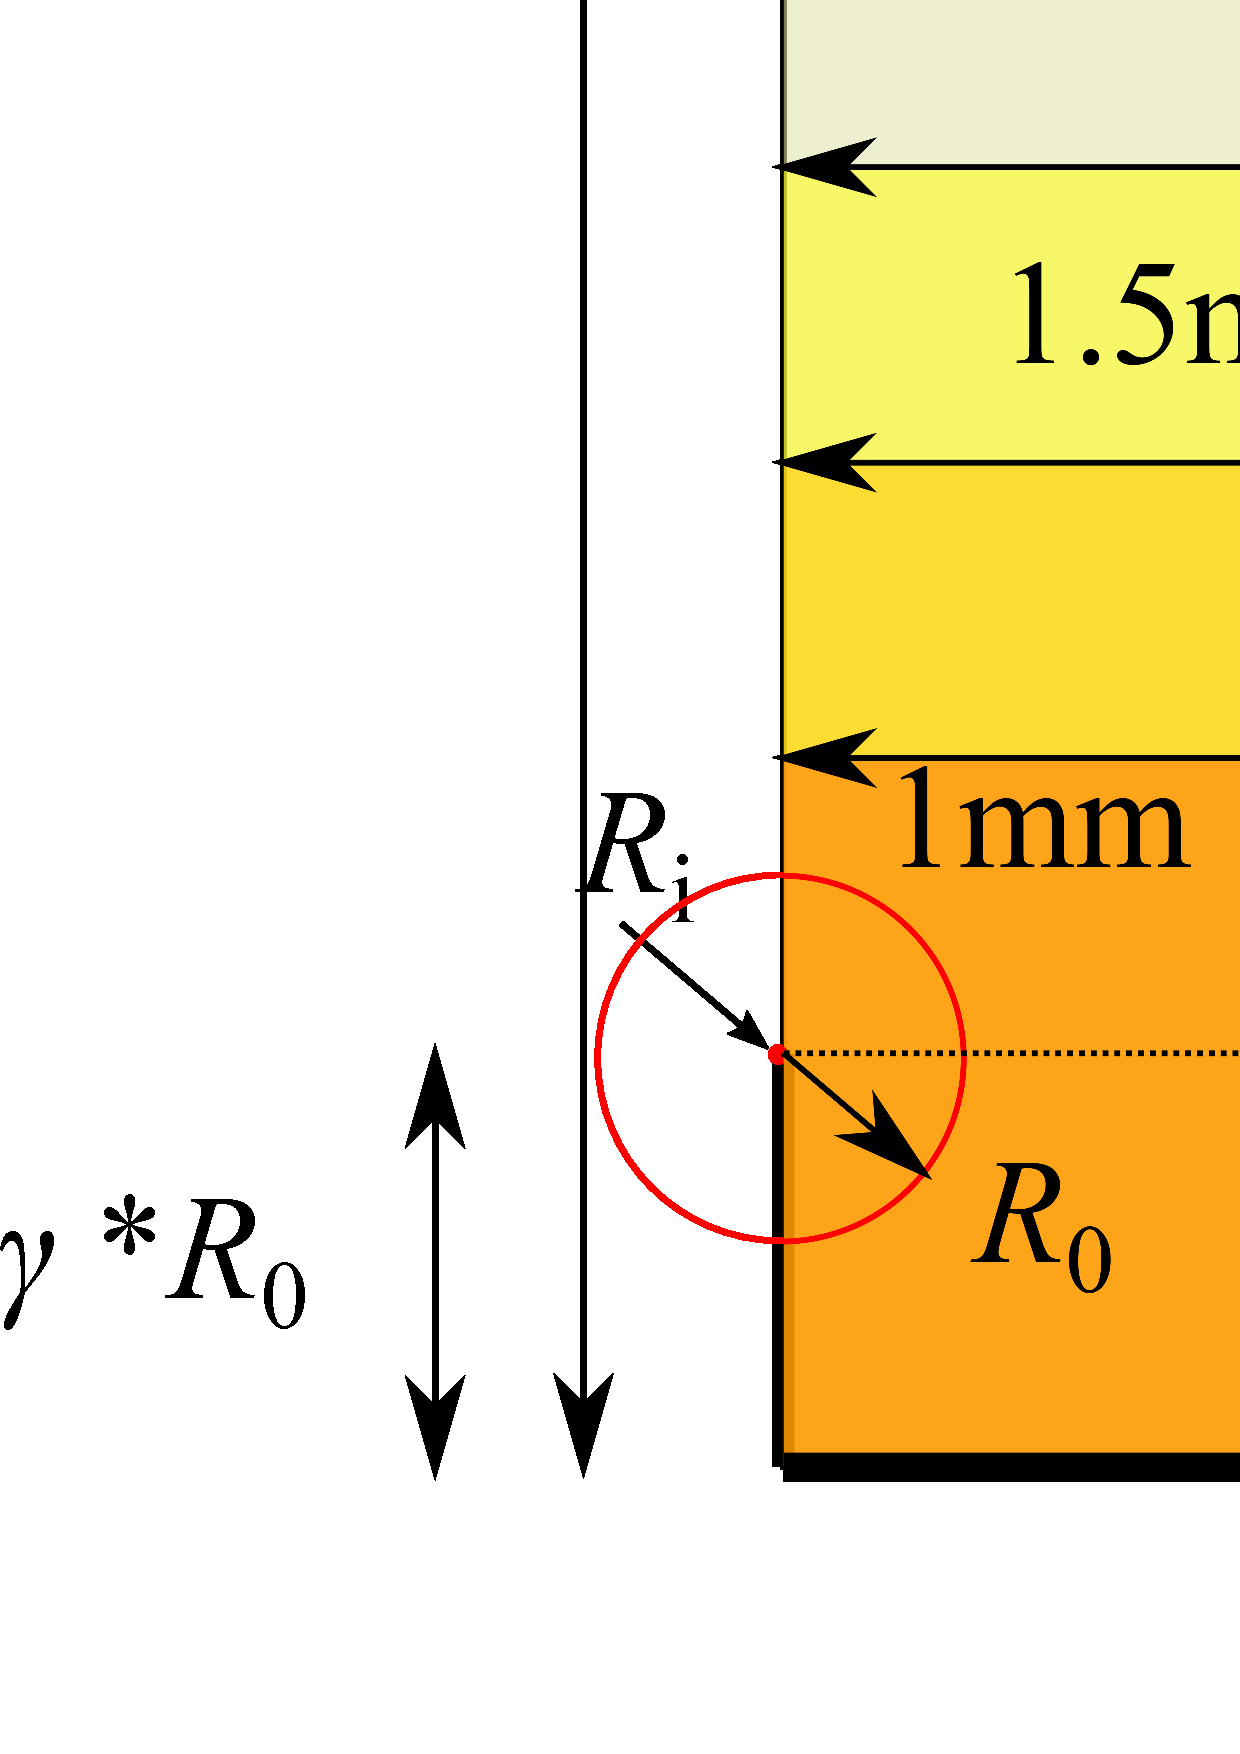
\includegraphics[width=0.7\linewidth]{img/solidwall.pdf}
    \caption{激光致空泡在固体界面附近的脉动计算域设置}
    \label{fig3.solidwallsetup}
\end{figure}

图\ref{fig3.solidwallsetup}显示了计算域的设置。对称轴仍使用对称边界,旋转面使用wedge边界,上边界和右边界都是“wavetransform”的无反射压力边界,和速度“pressureInletOutletVelocity” 流入流出边界。而固体壁面则使用“ZeroGradient”为压力和相边界,以“noSlip”为速度边界。网格密度和加密以及初始空泡设置,与上文中水与软物质界面附近空泡的设置一致。


\begin{figure}[h]
    \centering
    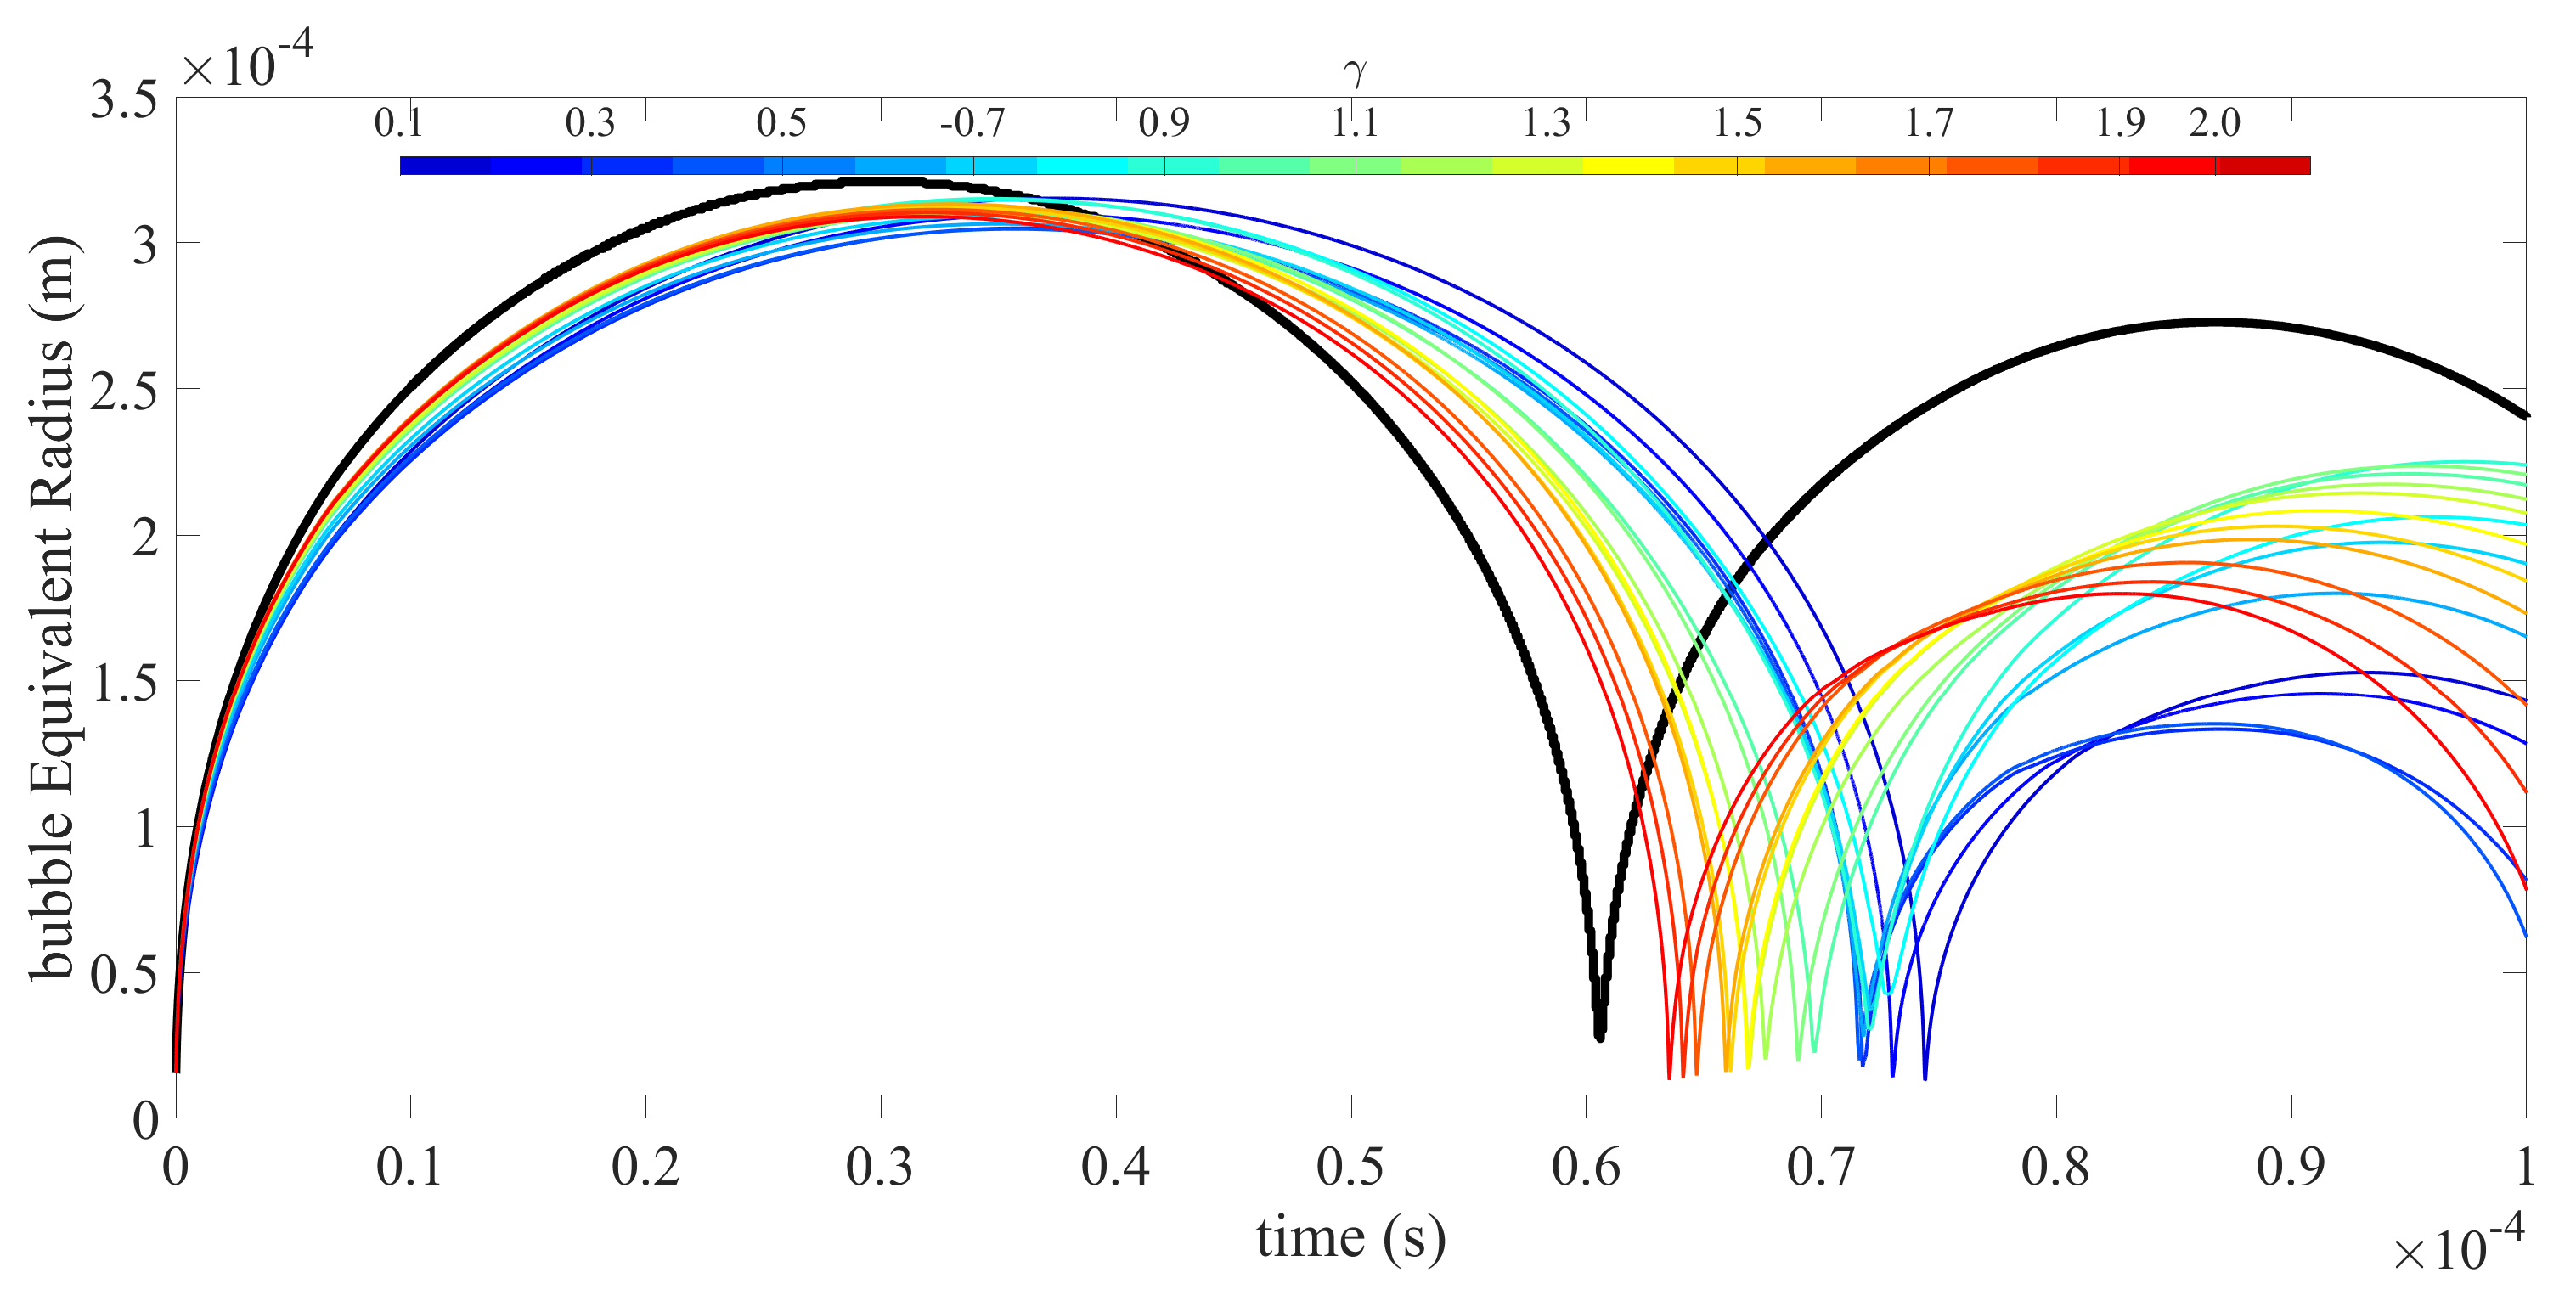
\includegraphics[width=1\linewidth]{img/fig3.solid.eps}
    \caption[空泡距固体界面不同相对距离情形下的泡半径对比图]{空泡距固体界面不同相对距离情形下的泡半径对比图,图中黑色实线为自由域中的模拟结果。}
    \label{fig3.solidradius}
\end{figure}

\begin{figure}[H]
    \centering
    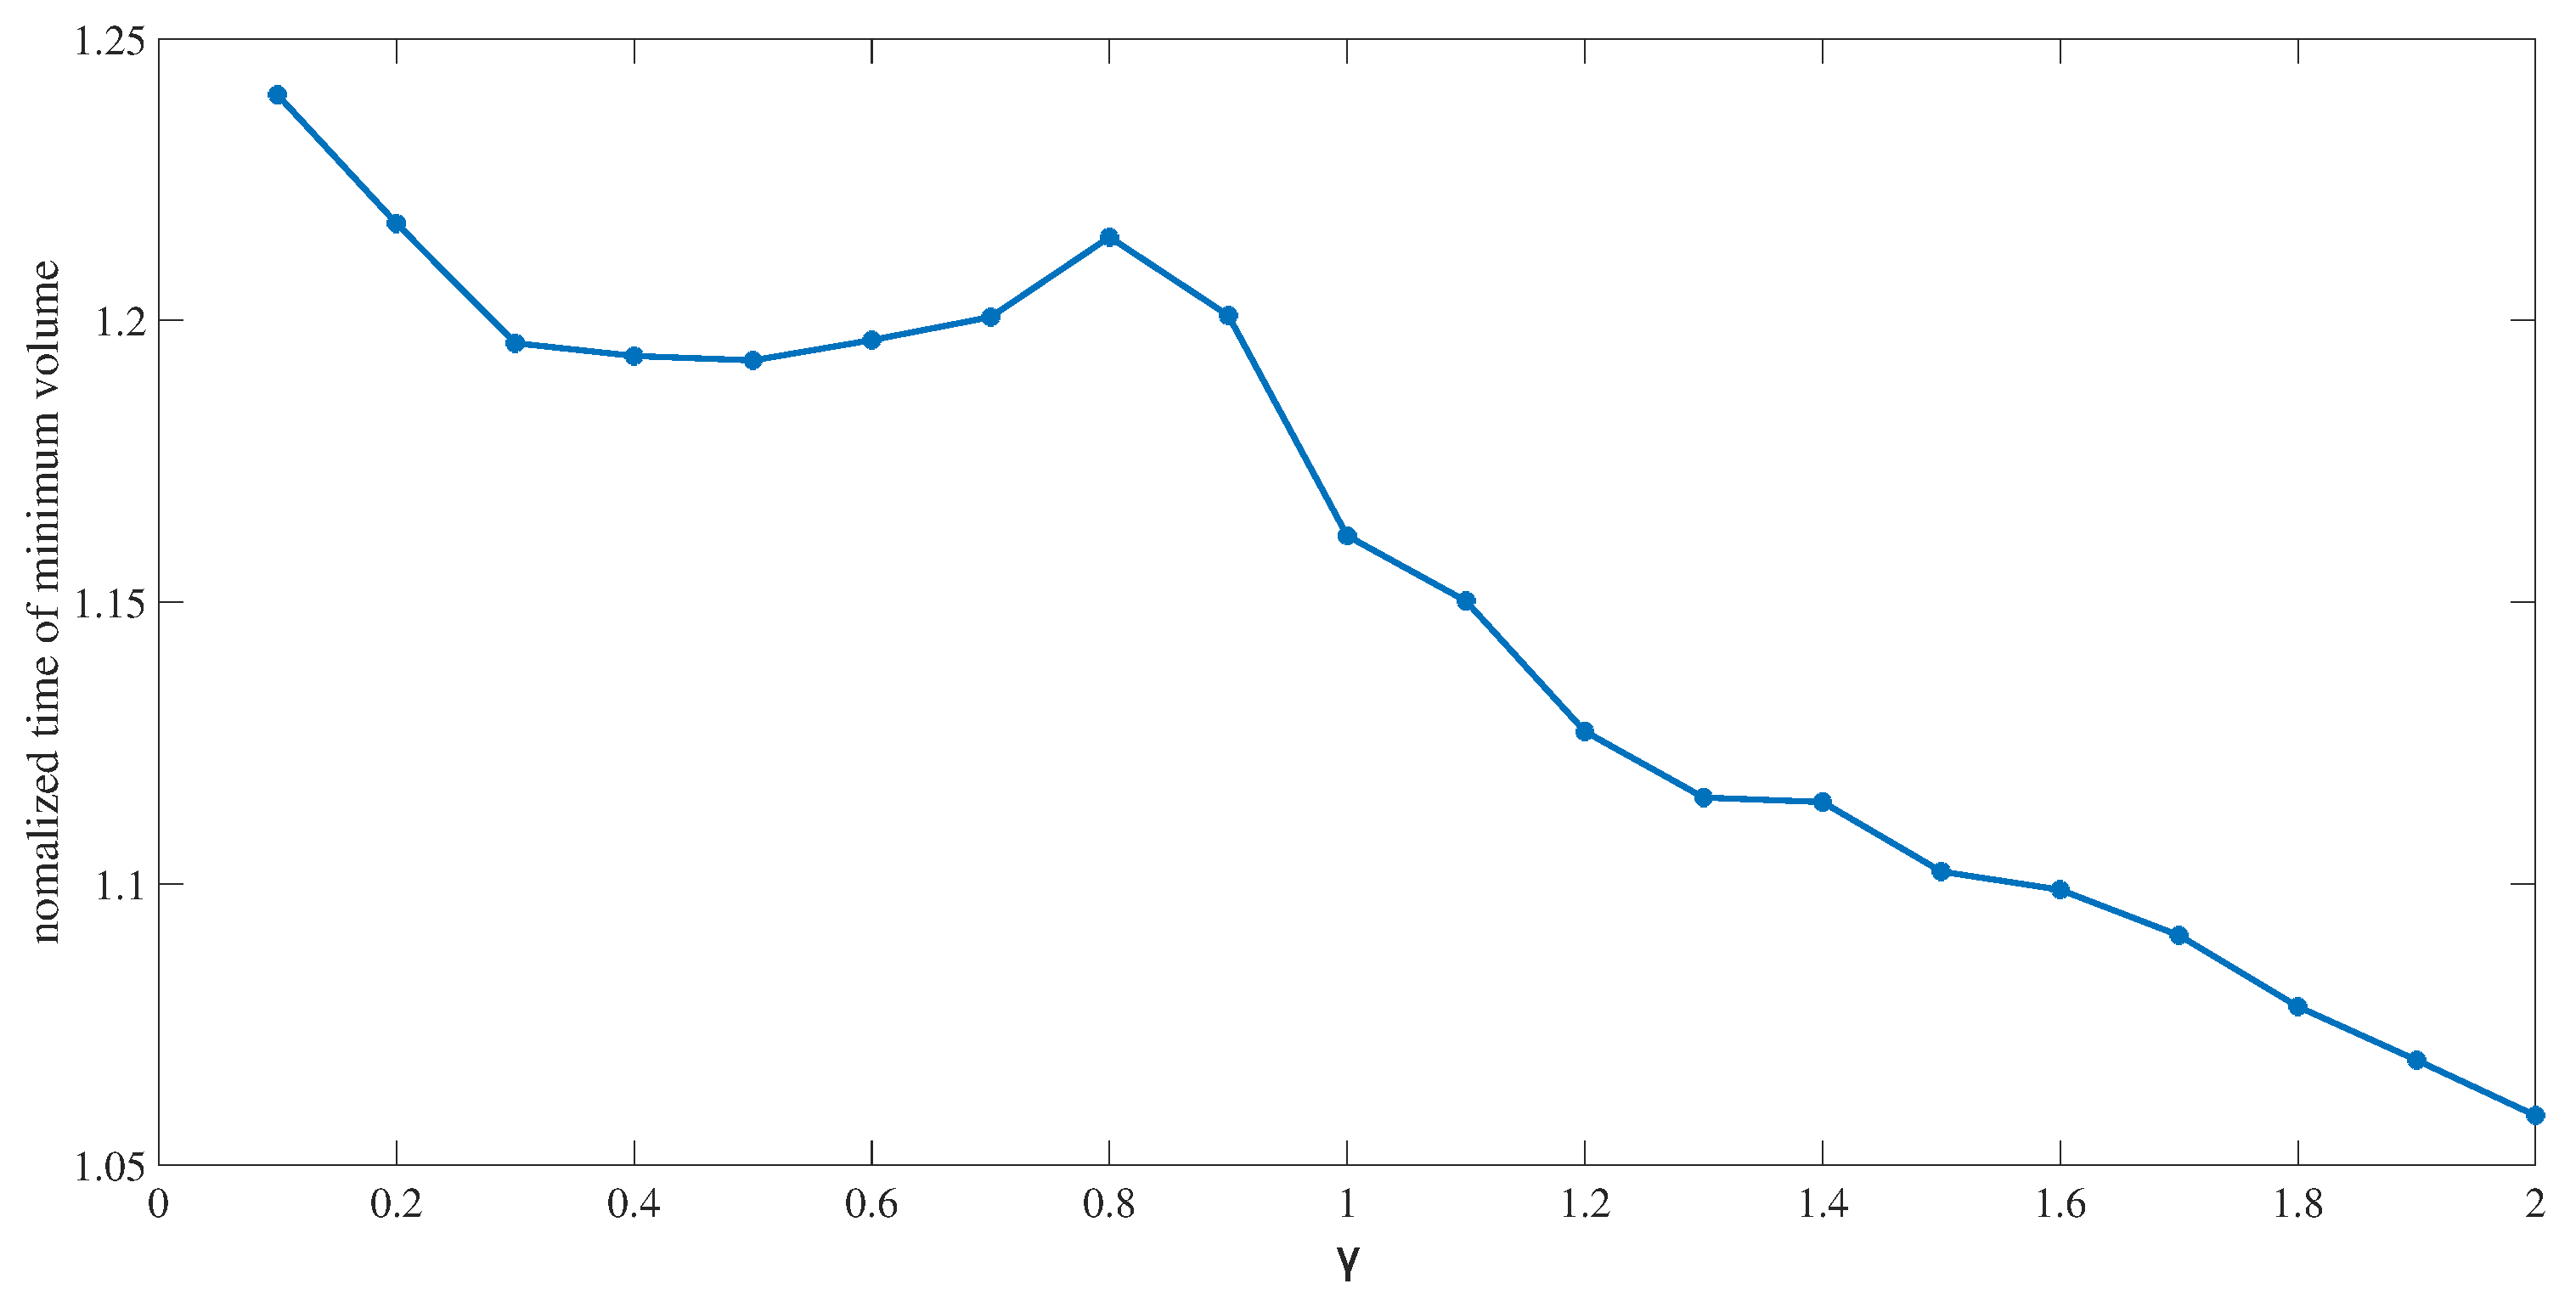
\includegraphics[width=0.9\linewidth]{img/fig3.solidnmlzedcollapsetime.eps}
    \caption[固体壁面附近空泡的归一化溃灭时间]{固体壁面附近空泡的归一化溃灭时间。归一化时间通过模拟计算中获得的体积最小时间除以自由域中的体积最小时间60.06$\mu s $获得。}
    \label{fig3.solidcolltime}
\end{figure}

图\ref{fig3.solidradius}中给出了空泡与固体界面在不同相对距离$\gamma$处的体积等效半径对比图。可以看到,在受固体制约的环境中,空泡的半径并没有达到其在自由域内能达到的高度。同时$\gamma$越大,也就是越接近自由的情况下,空泡的体积等效半径曲线越接近在自由域中的脉动。
在$\gamma\leq 0.2$,也就是空泡在界面附近时,空泡的膨胀曲线相比$\gamma> 0.2$等案例更高跨度更大。该情况可以见图\ref{fig3.solidcolltime}。图中清晰地表示了一个近似随着$\gamma$增大,归一化溃灭时间减少的趋势。这与越远离壁面越接近自由域的现实相符。
特别地,在$0.3\leq \gamma\leq0.8$区间内空泡的归一化体积最小时间有一个上升的趋势。这主要归功于空泡膨胀过程中与壁面接触后,形成粘滞作用。在空泡与壁面接触部分,边界层的存在对空泡的膨胀和收缩进行了一定地延缓。下文中将结合空泡的相-速度-压力云图给出解释。

在图\ref{fig3.solidcolltime}中可以简单的将曲线分为三个阶段,$A\,.$$\gamma\leq 0.2$的久溃灭时间阶段,$B\,. 0.3\leq \gamma\leq0.8$的溃灭时间缓慢增长的阶段,和$C\,.0.9\leq \gamma\leq2.0$的溃灭时间稳步下滑的阶段。在$A\,$阶段,过近的距离使空泡产生特殊的膨胀溃灭机制。其近似半球型的膨胀初期形状将很大的影响空泡的动力学特征。
在$B\,$阶段,因初始距离相对较在$A\,$阶段有明显的增大,从而在膨胀时虽然与壁面接触,但空泡也将受到壁面形成的推动作用。在这个阶段,空泡与壁面接触的时长也随着$\gamma$增长而减小,由此也表现出他独立的动力学特征。
在$C\,$阶段,空泡形成“常规的”射流动态,也就是空泡膨胀和溃灭都没有接触壁面,但受壁面影响形成压力梯度,从而形成射流。

下文将针对$A\,$,$B\,$,$C\,$三个阶段,各自选取一个案例对该种情况进行更细致的解释。其中$A\,$阶段,选取$\gamma=0.1$;$B\,$阶段,选取$\gamma=0.7$;在$C\,$阶段,选取$\gamma=2.0$。
%$0.3\leq \gamma\leq0.8$这个阶段主要是因为与壁面接触的时间越來越短而受到的限制作用逐渐减小。


\begin{figure}[h]
    \centering
    \includegraphics[width=0.9\linewidth]{img/solid2.0.png}
    \caption{空泡距固体界面$\gamma=2.0$情形下的相-速度-压力云图。}
    \label{fig3.gamma2}
\end{figure}
图\ref{fig3.gamma2}显示了$\gamma=2.0$时,空泡的相(白线表示空泡表面)-速度(右半部分图+箭头指示方向)-压力云图(左半部分)。从该图的第一栏可以看到,空泡在膨胀初期,如同自由域孤立单空泡一样各向同的膨胀。并逐渐释放泡内高压至水的饱和蒸汽压附近。在第三帧(18$\mu s$)中可以看到,空泡下部外缘形成较上部更宽的低压带。这个低压带在下一帧(27$\mu s$)中促使空泡向下移动,形成低速度区域的上移。

在第二栏的第一帧(31$\mu s$)中,空泡膨胀到最大泡半径。此时,低压带仍然存在,且速度矢量已经形成自上而下的趋势。可以看到,在空泡内部,速度指向为从上到下的。而在空泡外部上半部(北极),形成环流流向空泡上方。在空泡的下半部,速度指向壁面,并受壁面阻挡,而形成横向的外流。这时,空泡虽然处于最大泡半径时期,但已经形成了溃灭射流的潜在成因。在第二帧(45$\mu s$)中,空泡处于收缩状态。此时可见到空泡内部的下半部形成一个速度矢量的终点区域。这表明,空泡已经形成不均匀的收缩。在下一帧(54$\mu s$)中,空泡持续收缩,壁面速度继续提高。在第四帧(58$\mu s$)中,已经明显可见的形成了压力梯度,和速度梯度。就是空泡的外部的上半部分形成高压,而下半部分仍保持较低的压力。空泡内部的上半部分的速度继续提高,与下半部形成数量级的差别。此时,射流形成。

在第三栏中,第一帧(63$\mu s$)显示了空泡击穿前的流场。此时因空泡的持续收缩,水从上方持续的流向空泡上方,在空泡的上方形成一个高压区,这个高压区直接的驱动了射流的加速射向空泡低面。此时空泡内气体的流速达到440m/s。在第二帧(64$\mu s$)中,射流击穿空泡,空泡形成独特的花托(torus)状。在击穿过程中,因水体的碰撞形成巨大的能量释放,在碰撞过程中,向外辐射了一个冲击波。其在水中传播和反射,形成一个声速压力波。在第三帧(72$\mu s$)中,射流沿着对称轴方向继续前进。并在第四帧(81$\mu s$)中,射流撞击到固壁面。而此时射流的速度已经衰减到30m/s的量级。

在这个案例中,空泡形成“常规的”射流。就是在射流形成过程中,自空泡的北极先发生平化,继而向空泡内凹陷,然后发展成尖端点射流,除端点外边界拓扑没有形成突变,在射流击穿空泡后,继续前进了一段距离。这种“常规的”射流,有时发生在溃灭后期,有时发生在空泡回弹阶段。


\begin{figure}[h]
    \centering
    \includegraphics[width=0.9\linewidth]{img/3.solid0.7.png}
    \caption{空泡距固体界面$\gamma=0.7$情形下的相-速度-压力云图}
    \label{fig3.gamma0.7}
\end{figure}

图\ref{fig3.gamma0.7}展示了$\gamma=0.7$时,空泡的相(白线表示空泡表面)-速度(右半部分图+箭头指示方向)-压力云图(左半部分)。从第二帧($9\mu s$)中可以看到,空泡在膨胀初期就形成了膨胀的各向分化。在冲击波反射后,空泡的下方形成低压区,而空泡的上方则形成相对高压。但同时因固壁面的限制,空泡的下半部分(南极)出现平化,以及粘滞效应造成的低速度区。空泡的上半部分的膨胀速度远超下半部分,。同时因为压力的释放,在空泡的初始位置区域产生低速度区。空泡下半部分的外流场形成平行于壁面的发散流。第三帧($20\mu s$)空泡继续膨胀,但因为空泡的上半部分持续膨胀,内外压差降低并逐渐平滑,其速度逐渐下降。而同时,因固壁面的粘滞作用,空泡下半部分没有发生平化的区域,也就是没有直接面对壁面的区域速度没有发生较大变化。从而空泡的形状向帽子型逐渐演化。第四帧($31\mu s$)中,空泡达到最大泡半径。从速度图中可以看到一条蓝色带,其作为速度矢量的初始位置。这说明当前帧空泡外部的水惯性的外流,但空泡内部已经形成自上而下的速度趋势,此时异方向的速度值差别不大,均在1m/s左右。但可以看到,空泡南极的向外延展部分仍处于较高速度。即空泡下部仍保持膨胀状态。这是由于底部仍存在压差空间、壁面粘滞和惯性的共同作用。第五帧($45\mu s$)中,空泡南极的延展部分彻底平化,这是上一帧相对高速运动的结果。但同时,除这个延展接驳处仍作为速度矢量的终点方向外,因内外压差的驱动,全流场形成指向空泡的速度。空泡内部也形成自上而下的速度趋势。并在空泡下半部分转而指向上述接驳处。

在第二栏第一帧($57\mu s$)中,因全流场的运动的推动,空泡持续收缩。因北极附近形成更高的压力梯度,其速度逐渐开始提高。并且因空泡内部低压低密度气体也同时向壁面运动,空泡底部与壁面贴合得更加紧密。这也使空泡南极与壁面的接合部分成为全流场的速度终点。同样地,可以看到上文中的接驳处形成特殊的蘑菇伞盖状边缘结构。这种结构的底部是受固壁面的粘滞导致的收缩缓慢,以及当地作为空泡内部的速度出口影响而形成的。在下一帧中($65\mu s$),空泡北极附近因水的汇集而产生约4bar的高压。这个高压将驱动水射流的产生和射向空泡内部以及壁面。空泡内部也因水的持续汇集而形成高速的指向壁面的速度。值得注意的是,此时所谓的蘑菇状结构仍然存在,并将继续存在到溃灭。在第三帧($68\mu s$)中,射流在外界4.1bar的压力驱动下,撞击到空泡的南极。而蘑菇状特殊结构仍然存在,但有所收缩。下一个微秒($69\mu s$),因射流撞击壁面产生Blake Splash\cite{blake_art_1997, blake_acoustic_1999}(巴拉克喷溅)。在最后一帧($72\mu s$)中,空泡因喷溅和微射流而分裂,分裂后的每一部分单独溃灭时,都向外辐射了冲击波,并对隔壁空泡的溃灭进行了溃灭加强,形成较强的空泡南极位置的高压加强和多轮冲击波辐射。

在本例的这种情况下,空泡膨胀并与壁面发生贴合和黏连,导致空泡与壁面的接触面在水平方向上的膨胀时间较长,收缩速度较慢,形成特殊的溃灭结构。射流在击穿空泡下表面的几乎同时也到达壁面。在这种情况中,$\gamma$越大,接触面相对较小,但共同有类似的动力学过程。


\begin{figure}[h]
    \centering
    \includegraphics[width=0.9\linewidth]{img/3.solid0.1.png}
    \caption{空泡距固体界面$\gamma=0.1$情形下的相-速度-压力云图}
    \label{fig3.gamma0.1}
\end{figure}

图\ref{fig3.gamma0.1}展示了$\gamma=0.1$时,空泡的相(白线表示空泡表面)-速度(右半部分图+箭头指示方向)-压力云图(左半部分)。也是最为特殊的一种情况。
在首栏第一帧显示了空泡的初始位置,这时空泡几乎贴近固壁面。于是产生了在第二帧($ 1\mu s$)中,空泡形成的半球外型。此时,空泡的下表面贴合固壁面表面。而在边缘接驳处贴合位置尚未移动达到此处,其形成水膜层。此时就形成上文中特殊的蘑菇型结构。可以注意到,此时的速度在$Y>\gamma \times R_0$以上位置是呈扇形散射的。而在$Y<\gamma \times R_0$形成一个平行与壁面的流动。在空泡初始位置以下接近上述接驳处的空泡表面具有相对最高的速度。这是由于空泡初始能量的点源释放时,近固壁面方向受阻挡,物质在此处集中释放。于是形成下一帧($20\mu s$)中,此处的空泡界面追赶上其他方向的位置,形成半球型。但同时因固壁面的粘滞作用,这个接驳点仍然存在。空泡壁面此时仍受惯性驱动而继续向膨胀。而速度的集中释放位置也因固壁面粘滞的限制而上移到远离壁面的位置。在第四帧($36\mu s$)中,空泡到达其最大泡半径位置。此时空泡内外的速度都极小,将在下一时刻因外部高压的驱动而形成向内的速度。值得注意的是,上述的接驳处相比前一帧形成更加垂直的趋势。
第五帧($55\mu s$)显示了空泡收缩时的一个状态。靠近壁面的水平流推动空泡的下部垂直的移动,而空泡的上部则受辐射状汇聚的水流推动,形成扁帽式收缩。于是在水平流和辐射流的相交位置产生一种下部内嵌进上部的连接结构,有时也成为扭结结构。这种结构的早期诞生为后续现象的诞生确定最关键的因素。

第二栏中显示了空泡溃灭的一个序列。第一帧($64 \mu s$)中,近壁面的水平流持续推进壁面向对称轴运动。但壁面的粘滞作用使空泡贴在壁面部分很少的移动,也是靠近底部的部分对水平流的推动反应不明显。水平流的推动以及其被粘滞层挤压向上的移动和辐射流的推动,是内嵌结构处产生速度的叠加,形成高速点。这种速度的叠加在嵌入结构处持续演化,在第二帧($ 72\mu s$)中,其局部速度达到30m/s,较上一帧几乎翻倍。在本帧中,空泡壁面在水平流的推动和壁面粘滞的作用下,在空泡下部形成较大的倾斜度,同时在上方向下压迫的辐射流也对这个现象有贡献。另外值得注意的一点是,在空泡与壁面连接的地方,因当地存在连续的几个水滴。在泡外水体接触到这几个水滴后,立刻成为泡外水体的一部分。使空泡下边缘再次产生上文中特殊的蘑菇伞盖结构。此处蘑菇结构为在下一帧($ 73\mu s$)中表现出的冲击波负主要责任。而在此帧中,流域内的水持续想低压去域移动,内嵌结构处的收缩速度已经达到140m/s,与其他部位的40m/s产生较大的差距。随后在下一帧($ 74\mu s$)中,内嵌结构收缩撞击产生一个冲击波,这个冲击波在传播衰减后仍达到了160bar以上。而内嵌结构以上的空泡上部随结构的撞击而脱离空泡本体,形成一个微气泡。而在内嵌式结构撞击后,形成一个高速的朝向上下两个方向的射流,但因为上部本就是水体环境,只表现为高压局部。而空泡内则形成一个针状射流,其速度可以达到近1000m/s,在图中表现为衰减后的830m/s。同样的现象,Fabian和C-D,Ohl实验发现并解释了该现象\cite{reuter_supersonic_2021},如图\ref{fig3.needlejet}所显示的。在图\ref{fig3.gamma0.1}最后一帧中,射向空泡的射流击穿空泡,撞击壁面,沿着壁面方向延展,并发射了一个冲击波(传播出视野)。而被嵌入式结构截断的微空泡在向上方向的射流推动下继续向上运动及回弹。


\begin{figure}[h]
    \centering
    \includegraphics[width=0.9\linewidth]{img/fig3fabiandieter.jpg}
    \caption[实验发现的内嵌式结构和针状射流]{实验发现的内嵌式结构和针状射流\cite{reuter_supersonic_2021}。}
    \label{fig3.needlejet}
\end{figure}

在这种情况下,空泡形成一个半球型,其不是简单的形成一个自上而下的射流,而是形成特殊的内嵌式结构,空泡的这个结构在左右方向上持续收缩,最后撞击产生高压并形成向下的超高速射流。在这之前,空泡一直没有形成射流初始状态的内凹。



\begin{figure}[h]
    \centering
    \includegraphics[width=0.7\linewidth]{img/figkink.jpeg}
    \caption[实验发现的内嵌式结构和射流的分野]{Fabian 和CD, Ohl实验发现的内嵌式结构和射流的分野\cite{reuter_supersonic_2021}。}
    \label{figkink}
\end{figure}



%$\gamma$ 对脉动形式的影响
空泡在距离壁面不同$\gamma$ 时表现出不同动力学特征。当$0.9\leq \gamma\leq2$(本文中所做案例的上限)时, 射流在击穿空泡后射向壁面,且空泡在射流击穿前其下半部分保持较好的球性。当$\gamma=\{0.3,0.4,0.5,0.6,0.7,0.8,\}$ 时,空泡粘着在壁面上,并形成特殊的空泡结构。射流在形成后指向壁面,并促使射流击穿空泡的同时也接触壁面,从而形成BlakeSplash。$\gamma=\{0.1,0.2\}$时,空泡形成一种嵌入时结构,这种嵌入式结构在收缩时碰撞并随之形成高速针样射流。
这与实验结果\ref{figkink}\cite{reuter_supersonic_2021}的结果一致。


\begin{figure}[h]
    \centering
    \includegraphics[width=0.9\linewidth]{img/solidtime.eps.pdf}
    \caption{空泡距固体界面不同相对距离情形下的射流击穿空泡时间和射流到达固体壁面的时间}
    \label{fig3.jettime}
\end{figure}

在以上三种情况中,都产生了各自特殊情况的射流。
图\ref{fig3.jettime}显示了空泡距固体界面不同相对距离情形下的射流击穿空泡的归一化时间和射流到达固体壁面的归一化时间。对大相对距离的情况,也就是$\gamma>1.7$时,射流击穿的归一化时间相当接近1.0,也就是射流击穿时间和自由单空泡的溃灭时间接近。也可以理解成,在这种情况下,空泡的射流击穿是在空泡的溃灭末期形成的,即空泡溃灭和空泡射流几乎同时。可以认为,$\gamma$越大这种同时性会越來越好。这与\ref{chapter1.2.2.2}中使用$\zeta$预言的结果一致。在$\gamma>0.7$时,空泡击穿的时间是递减的,也就是越脱离壁面的影响,空泡的击穿时间越接近自由空泡。而空泡到达壁面的时间是递增的,这与空泡离壁面位置越远到达壁面的时间越长的逻辑是一致的。$0.3\leq \gamma\leq0.8$范围内,空泡的膨胀贴近壁面,射流击穿空泡自身和到达壁面的时间几乎一致。而$\gamma\leq0.2$时,空泡表现出半球型膨胀和收缩,其空泡的体积等效半径与其他空泡类似,但因半球型而形成较大的上下空泡面距离,其形成的针状射流,时间较晚但速度较快。


\section{本章小结}


本章主要探讨了基于可压缩多相流模型的空泡在水-气、水-油、水-固界面附近的脉动情况。针对空泡距离不同界面不同位置做了空泡动力学分析和射流模式的分析。
在水气界面形成三种不同的相互作用机制:爆破型、皇冠射流型、和凸起型。
在水油界面则分成了断裂式溃灭和射流式溃灭。而其中断裂式溃灭又可以细分为断裂接触式和断裂射流式。
在水固界面也因三种空泡的脉动形式而形成多种射流机制:常规射流溃灭,和针状射流溃灭。常规射流又可以细分为空泡接触壁面和不接触壁面两种机制。

文中对空泡动力学和形态学进行了详细的解释,并分析了针对空泡与界面的距离对空泡与界面相互作用的规律性现象。

本模型也可应用于计算更多种不同界面形状和不同物性的空泡脉动。



%
\chapter{激光致自由域内同相线性三空泡的动力学}

\section{单帧瞬态曝光照相系统和多激光空泡的实现}
\begin{figure}[H]
    \centering
    \includegraphics[width=\linewidth]{img/fig4.1.png}
    \caption{多空泡单帧瞬态曝光阴影法照相的实验设置。}
    \label{fig4.1}
\end{figure}




本作中用于研究激光致对称线性排布的三个同相空泡的实验装置如图 \ref{fig4.1}所示。
为了产生空泡,采用了 1064 脉冲激光波长: 1064nm; 最大单脉冲能量: 1J;
脉宽:10ns)。单脉冲能量从 100mJ 到
1J,激光器能量浮动±5\%。分波片把激光分成两部分。一部分用于监测能量,一部分被三点分波片
(DOE,Diffractive Optical Element; Holo/Or TS-245-I-Y-A)
分成同一平面内等角的三束光束。三个反射镜将三束光反射到一个用于聚焦并获得规则空泡的消球差透镜
($f=30\mathrm {mm}$)
中心。如此,可以在焦平面处获得与反射镜、透镜中心同平面的竖直排列的焦点。在焦点处,水箱
(熔融石英, $50\times 50 \times 50 \mathrm{mm^3}$)
中的去离子水被击穿,并产生等离子体,其后演化成空泡。可以通过遮掩特定的光束来获得单个或者两个空泡。实验中,可以通过改变反射后的激光的入射角度和镜片间的距离来获得不同的焦点距离。

为了对空泡脉动的快速过程进行成像,使用了单帧工业相机 (Imi, imc7017g)
和短脉宽 (Nd: YAG,波长: 1064nm; 脉宽: 2.5 ns) 照明激光。照明激光经过
KTP 晶体倍频获得 532nm
的照明脉冲。照明脉冲经过衰减并扩束。然后,此照明光携带空泡信息照在 CCD
上。探测光与激发光和空泡排列垂直。延迟信号发生器 (Stanford Research
Systems Inc., DG535) 用来触发 CCD
和相机。通过光电二极管能够获得击穿闪光和照明光的时间延迟,以此来获得 CCD
收集到的空泡信息的具体时间。

在实验中,最大空泡的半径通过在空泡阵列实验前的用相同激光能量的孤立球形单空泡实验获得\cite{han_dynamics_2015,fong_interactions_2009}。记录了单空泡的脉动和溃灭时间。实验结果符合 Keller-Miksis
模型。溃灭时间波动±5\%。如此,理想的最大空泡半径 $R_0$
通过溃灭时间的中值而获得 \cite{Kroninger2010}。与通过阴影面积获得的结果
\[R_{\text{0}}=\frac{\sqrt{\text{max(Area)}}}{\pi}\,,\]
比较,差别十分微小,此处忽略之。空泡的初始距离 $D_0$ 通过低于 100ns
的早期帧获得,此时等离子体正在复合并转化成蒸汽\cite{zhang_transient_2016}。



\begin{figure}[H]
    \centering
    \includegraphics[width=0.7\linewidth]{img/fig4.2.png}
    \caption[空泡设置及参数定义示意图]
    {空泡设置及参数定义示意图。左上角的一帧显示了孤立单空泡情景下的最大泡半径状态。红色虚线显示了空泡的外接圆。阴影面积可以用来计算空泡半径。同时此半径也用
Keller-Miksis 模型中的 Rayleigh 时间做了验证。左下帧显示了一例(
$\gamma$
=0.45)初始击穿状态的照片。图中黄色和绿色线段的平均长度表示了空泡的初始距离,$D_0$。右边图像展示了
$\gamma=0.8$
时的一幅代表帧。红色虚线是边缘泡的最小外接矩形。蓝色虚线则代表了中心泡的最小外接矩形。绿色线段是定义的
$B\text{-verge-outer}$,而黄色则是
$B\text{-verge-inner}$。淡蓝色是中心泡的次轴,$B\text{-center}$。橙色线段代表了不同位置空泡的主轴,即
$2A$。$D$,空泡间距则未在图中标注,其是通过图中 $A$,$B$
线段的焦点间的距离获得的。}
    \label{fig:4.2}
\end{figure}

我们在本章中重点关注了空泡的大小和距离。空泡在某个时间的半径
$R$,是通过阴影面积 $\pi R^2$
来计算的。在孤立的单空泡脉动过程中,获得最大空泡半径 $R_0$,初始距离
$D_0$ 是两对相邻击穿点距离的平均值,如图 \ref{fig:4.2}
所示。为了规范化,无量纲常数 $\gamma$ 定义如下:
\[ \gamma=\frac{D_{\text{0}}}{2R_{\text{0}}} \\\,,(4.1)\]

其他在动力过程中的重要参数 $A$,$B$ 如图  \ref{fig:4.2}
所示。因为相互作用,空泡在脉动过程中逐渐失去球状。根据其二维图案,$A$
是半主轴长度,$B$
是半次轴长度。而通常空泡的形状是不规则的。我们把空泡的最小外接矩形的近水平轴定义为主轴。将图形重心到到外水平轴的距离定义为
$B_\text{outer}$,$B_\text{inner}$
定义为图形重心到到内水平轴的距离。两个外围空泡平均后得到一组
$A$,$B_\text{outer}$,$B_\text{inner}$。中间空泡的 $B$
是重心到外接矩形的上下边缘的距离平均值。

为了理解整个过程中的空泡变形,引入了一个规范化的参数$C$,圆度。它定义如下:

\[C=\frac{\text{等面积圆的周长}}{\text{空泡的周长}}=\frac{2\sqrt{\pi S}}{P_{\text{b}}}\,,\]

$S$ 代表了阴影图中的空泡面积,空泡周长为
$P_\text{b}$。分子是与图中空泡具有相同面积的圆所具有的周长。这时,完美的圆的圆度为
$C=1$。空泡形变离圆越远,其值越小。

为了追踪空泡的相对位置变化定义一个无量纲数~$\tilde{D}$:

\[\tilde{D}=\frac{D}{D_{\text{0}}}\,,\] $D$是实时距离,~$D_0$是图
2中显示的初始中心和边缘空泡距离.

本章中,实验研究了五组 $\gamma$ 值 (
$\gamma=0.45=1.35\,\text{mm}/(2*1.5\,\text{mm})$,
$\gamma=0.80=2.40\,\text{mm} /(2*1.5\,\text{mm})$,
$\gamma=1.0=3.0\,\text{mm} /(2*1.5\,\text{mm})$,
$\gamma=1.47=2.94\,\text{mm} /(2*1\,\text{mm})$,
$\gamma= 1.93=3.85\,\text{mm} /(2*1\,\text{mm})$)。这些情景代表了理想状况下,相邻的两个空泡的图案相互覆盖,相互挤压,相互接触,距离较近,和距离较远。整个过程中每
$5\mathrm {\mu s }$间距采集不少于 20
次,以此来追踪给定条件下的多空泡动力学。

\section{三空泡阵列的形变及溃灭}

本节中,典型案例的实验结果将通过阴影法摄像术获得的结果展现。由于空泡间距较近,流体力学作用占据主导,其情况复杂,将在后续章节中给出基于OpenFOAM的模拟计算结果及讨论。本节简单地将泡间相互作用考虑成空泡的声辐射对其他空泡的影响。这种简化普遍应用在空泡群的研究中\cite{brennen_cavitation_2003,ohl_shockwave_2013,lv_experimental_2019}。
在本研究中占据主导作用的参数是$\gamma$,也就是相邻空泡的无量纲距离,定义如公式(4.1)所示。
下文中给出的实验图(\ref{fig:4.3},\ref{fig:4.5},\ref{fig:4.7},\ref{fig:4.9},\ref{fig:4.11})显示了关于三个对称线性排布的同相空泡的动力学的实验照片,也即上述五个典型相对距离的案例的时序阴影法照片。这五个案例的不同
$\gamma$ 和相邻空泡孤立膨胀情况下的几何关系可以针对性的总结如下:

案例一:大 $\gamma$(如图\ref{fig:4.3} 
所示,$\gamma=1.93$)。此时孤立膨胀到最大的空泡几何距离相邻空泡较远。空泡边缘的间距大约是两倍直径。此时空泡间存在着本节中五种情况最弱的相互作用。

案例二:大 $\gamma$(如图\ref{fig:4.5} 
所示,$\gamma=1.47$)。此时孤立膨胀到最大的空泡几何距离相邻空泡较近。空泡边缘的间距大约是两倍半径。此时空泡间存在着本节中五种情况次弱的相互作用。

案例三:中等 $\gamma$(如图\ref{fig:4.7} 
所示,$\gamma=1.0$)。此时孤立膨胀到最大的空泡几何与相邻空泡相互接触。此案例有本研究五种情况中中间强度的相互作用。

案例四:小 $\gamma$(如图\ref{fig:4.9} 
所示,$\gamma=0.80$)。此时孤立膨胀到最大的空泡几何相互挤压,也就是在达到最大泡半径之前就相互接触,但边界没有超过对方的中心。此情景有本研究中次强的相互作用。

案例五:小 $\gamma$(如图\ref{fig:4.11} 
所示,$\gamma=0.45$)。此时孤立膨胀到最大的空泡几何相互覆盖,即空泡距离非常近,甚至在膨胀早期就产生挤压。在孤立几何上,最大泡半径时,其边界超过了对方的重心。这种情况有本实验中最强的相互作用。

\begin{figure}[H]
    \centering
    \includegraphics[width=0.7\linewidth]{img/fig4.3.png}
    \caption{案例一,大$\gamma$($\gamma=1.93$)情况的最弱相互作用。}
    \label{fig:4.3}
\end{figure}


\begin{figure}[H]
    \centering
    \includegraphics[width=0.7\linewidth]{img/fig4.4.png}
    \caption{案例一的参数曲线。}
    \label{fig:4.4}
\end{figure}


在本章的上图和下图中,$t$ 是具体时刻,$T_0$
是自由域中单空泡的第一脉动周期时长,而$T=t/T_0$
则是归一化时间。通常,自由域中孤立的空泡在$T<0.5$ 膨胀,并在$T=0.5$
附近时达到最大泡半径,随后收缩,并在$T=1$时溃灭。

图\ref{fig:4.3}  和 \ref{fig:4.4}显示了案例 1,$\gamma=1.93$ 的结果。在图 \ref{fig:4.3}
中,第一帧是空泡的初始阶段。此情况下,初始分离距离较远,泡间的相互作用较弱。根据时间序列图,泡的形变主要受初始形状的影响。在膨胀期,如上栏
2、3、4
帧阴影图的面积,中间泡的略小于边缘泡。这意味着中间泡的相位略提前,边缘泡先于中间泡达到最大泡半径。
此处相位看做空泡所处运动状态在一个运动周期内的相对位置,
\[\varphi=\pi(\frac{t_\mathrm{exact}}{T_\mathrm{oscillation}}) \]假设$\pi$是一个周期,则$\pi$/2指半周期,此时$\pi$和$\pi$/2就是其相位\cite{fong_interactions_2009}。运动周期变长,意味着到达某个相位的时间延后,某个时间对应的相位提前。此处我们就采用相位被推迟指一个周期性运动的周期变得更长。在收缩时,边缘泡的相位也晚于中间泡。同时辐射的压力波和张力波造成的相互作用效果也逐渐显现。如下栏第一帧所示,空泡被拉长,边缘泡的外缘产生平化现象,其收缩速度较内缘快。如下栏第二帧所示,边缘泡产生指向中间泡的射流,中间泡仍保持较大的。在下栏第三帧中,边缘泡溃灭并产生冲击波,但中间泡仍然生存并继续收缩,在第四帧后溃灭。同时因为射流的原因边缘泡的再次膨胀位置向中间移动。

图 \ref{fig:4.4} 是空泡规范化的半径 $R$ 和各轴以及圆度关于时间变化的曲线图。半径
$R\,$ 的分布相对 Keller-Miksis
曲线更扁更宽。这意味着空泡的脉动受到抑制。在泡的相互作用过程中,泡能转化为单空泡势能减小,使泡不能到达其原最大半径
$R_0$,并使其相位推迟。因为中间泡同时受到两边泡的影响,而两边泡因为受到隔绝作用\cite{bremond_interaction_2006,dear_study_1988,Dear1988a},只受中间泡的影响,所以中间泡受到的抑制更加明显,使其最大泡半径小于边缘空泡的最大半径,相位推迟更多。此处因为泡能有限,相位推迟还伴随着最大泡半径值的减小。

在膨胀期$A$、$B$轴差别不大。但在两种位置的泡都进入收缩期后,因为辐射负压的原因会对其他泡产生拉伸作用,主要作用在$B$轴上,使$B$轴变长。中间泡的被拉伸最明显,其$A\,$,$B$轴都较边缘泡长。同时因为边缘泡产生凹陷形变,基于最小外接矩形的$B_\mathrm{inner}$和$B_\mathrm{outer}$不能准确描述其形变。从圆度C图上看到边缘泡在收缩末期,即$T>1.05$处,圆度$C$变小,而中间泡则在$T=0.8$
后因为拉伸而失去圆度$C$.

总体上案例1的脉动与单空泡脉动较为类似,但相位稍微延长,最大泡半径略小,且在溃灭前会产生较大形变。

\begin{figure}[H]
    \centering
    \includegraphics[width=0.7\linewidth]{img/fig4.5.png}
    \caption{案例二,大
$\gamma$ 情景,($\gamma=1.47$)。次弱相互作用情景的结果。}
    \label{fig:4.5}
\end{figure}


\begin{figure}[H]
    \centering
    \includegraphics[width=0.7\linewidth]{img/fig4.6.png}
    \caption{案例二中的各参数。}
    \label{fig:4.6}
\end{figure}


图 \ref{fig:4.5} 和 \ref{fig:4.6} 是案例二,$\gamma=1.47\,$
的结果。整体结果与案例一类似,但因为泡间的间距更小相互作用更强,使一些效果更加明显。但初始阶段影响十分小如第二帧几乎毫无影响。比如相位延迟更加明显。因相互作用产生的对相位的抑制也与
案例一 类似。对比图 4.3 和 4.5 下栏的三四两帧,案例二
的两种泡溃灭时间都更晚,中间和边缘的时间差更大。因双重抑制产生的中间泡相位落后更加明显,如产生拉伸,产生射流溃灭的
$T$ 更晚。

从$R$图中也可看出案例二的$R$更宽更窄的回弹在$T>1.1$处,而案例一的在$T~=1.1$处。案例二$R$
能达到的最值也略小于案例一,且达到时间也较晚,这是抑制造成的$R$
曲线相位延迟。中间泡和边缘泡的差异也有所扩大。

从AXES 图中能看到,
$B_\text{verge}$,$A_\text{verge}$与$R$基本上同步地到达最大收缩与最小回弹。中间泡的$A$和$B$
在膨胀阶段与$R$同步而小于边缘泡的$A$、$B$。与边缘泡的轴相比$A_\text{center}$更扁且更宽。$B_\text{center}$在$T=0.65$处与其他轴曲线分离并保持持续高位直到$T=1$后逐渐减小,即案例二的中间泡的在竖直方向上拉长。

相比案例一变形更加明显。边缘泡因为射流的原因其$C$在溃灭后期$T= 1.0$迅速变小,其恢复期因为多泡干扰而不稳定过程也保持较小的$C$,而中间泡因为其被拉长在$T=0.65$处开始缓慢下降,并在溃灭阶段急剧减小。相比案例一,整体变形更加明显,变形时间$T$也提前了。

\begin{figure}[H]
    \centering
    \includegraphics[width=0.8\linewidth]{img/fig4.7.png}
    \caption{中等$\gamma$,$\gamma=1.0$,中等相互作用的实验结果。}
    \label{fig:4.7}
\end{figure}


\begin{figure}[H]
    \centering
    \includegraphics[width=0.8\linewidth]{img/fig4.8.png}
    \caption{例三的轴参数。}
    \label{fig:4.8}
\end{figure}


图\ref{fig:4.7} 和 \ref{fig:4.8} 是案例三,即 $\gamma=1.0$
时的情景。由于间距更近,相互作用更加明显。如第三帧所示,中间泡的膨胀受到抑制。边缘泡内边缘产生平化并形成因形状变化的重心的偏移。第四帧所示,边缘泡到达最大泡半径附近,但中间泡的相位落后较大,未到达最大。两组泡都产生明显的形变,相对面平化更加严重,
边缘泡的重心向内移动。第五帧所示,中间泡达到最大泡半径附近时,边缘泡开始收缩。在第四到第五帧之间,三泡并没有形成接触,中间的水层较厚,约为
$0.3-0.4*R0$。边缘泡收缩,形成对中间泡的拉伸,如第六帧所示。同时边缘泡的内(inner)和外(outer)两轴的泡外压不同,在外边界形成向内的射流。相互作用持续影响,泡间相位差逐渐积累
(此处就指相位差扩大)。中间泡在垂直方向上持续增长,而水平方向收缩与边缘泡大概同步。如第六七帧所示。最后边缘泡被射流击穿,随后溃灭并回弹,而中间泡在水平方向上溃灭并回弹,如第八帧所示。这两个溃灭时间较案例二更晚。

图七是显示了归一化后的半径轴和圆度相对时间的变化。表示击中的点分布的更加分散,并且随着T的增大而变得更加宽。空泡膨胀初期跟随Keller-Miksis模型,在膨胀的压力波开始影响彼此后,膨胀因为内外压差减小而减缓膨胀。$R$的曲线不再是关于$T=T_x$(在Keller-Miksis模型中,
$T_x$=0.5)的对称曲线,变化更加平缓,跨度更加大。内外泡能达到的最大泡半径与Keller-Miksis模型的差相比案例二变得更大。边缘泡在$T=0.5$到达其$R$最大,而中间泡则在$T=0.6$前后到达最大。中间泡保持了较大的R时间显著变长,边缘泡也有一定的延长。这是对应于收缩形成的张力波的相互影响。

整体上边缘泡轴的变化与$R$类似。这也与$C$较高结果一致,其圆性较好。膨胀阶段中间泡的$A$、$B$小于边缘泡的$A$、$B$。中间泡在其到达最大泡半径的$T=0.6$处开始有较明显的变化。$A$轴的减缓速度减慢,其高度高于边缘泡的两个轴,因为没有产生黏连且受舒张波的影响较大。其$B$轴持续近线性增长至$T=1.1$,然后由于溃灭的发生而产生骤降。相比与案例二,这个骤降的转折发生的更快且相位更晚。$B_\text{verge-outer}$
大于$B_\text{verge-inner}$表示边缘泡的重心向阵列中心移动,从而使更靠近阵列中心的部分横向更宽。($B_\text{verge-outer}$
和$B_\text{verge-inner}$ 的差一定程度上体现了形变造成的重心移动。)
$A$、$B$轴表现的中间泡的这种形变体现在 $C$ 上表现为自 $T=0.6$
开始逐渐平滑的变小,并在溃灭时达到最小。

\begin{figure}[H]
    \centering
    \includegraphics[width=0.7\linewidth]{img/fig4.9.png}
    \caption{案例四: 小 $\gamma$
($\gamma=0.80$),次强相互作用的实验结果。}
    \label{fig:4.9}
\end{figure}


\begin{figure}[H]
    \centering
    \includegraphics[width=0.7\linewidth]{img/fig4.10.png}
    \caption{案例四的轴参数图}
    \label{fig:4.10}
\end{figure}


图 \ref{fig:4.9}和\ref{fig:4.10} 显示了案例四,即 $\gamma =0.8\,$
的结果。从上栏的第二帧看到,空泡的初期演化空泡仍然形成较好的球形。但在空泡在受到其他空泡形成的压力波影响后,开始出现相位的不同。在第三帧中,边缘泡明显大于中间泡。这是上文所述的抑制的作用。中间泡和边缘泡形成较明显的相位差。同时因为膨胀受到抑制,相接触部分产生平化,并产生一定的推动。在第四帧中,边缘泡开始收缩变小,在静水压和拉力与泡内压的共同作用下,使中间泡达到最大并保持较长时间。因为这种相互拉伸,空泡的间距实际上是减小了。在下栏中,中间泡开始收缩,但因为同时受到来自边缘泡的拉伸,而形成独特的柱状结构。其相对面发生平化,而从水平对称轴亦即中间位置开始产生变化
(此处指收缩)。在下栏第二帧中,泡间形成明显的水膜,边缘泡因为射流带动并向内塌陷,中间泡的水平对称轴方向的收缩更加明显。边缘泡与中间泡相对面受到中间泡的拉伸,越靠近竖直对称轴,越靠近相对位置,相位就越慢。从而在外部形成向内的射流。下栏第三帧中,边缘泡的射流击穿边缘泡,并射入中间泡,而中间泡继续收缩,形成显著的细腰形状,后期将由此位置破裂,并形成水锤压向外辐射冲击波。下栏第四帧中,边缘泡完全溃灭,残余气体与中间泡的残余气体混合在一起。中间泡的中间位置相位更前,形成二次膨胀,但因为不稳定,中间泡实际上解体形成复杂的气体残余状态。形成射流和溃灭的时间分别都大于案例三情况下的。在
$\gamma$
足够小的情况下,空泡在脉动过程中可能出现自中心向外蔓延的黏连,但是仍能看到明显的边缘分界缺口,如本例中第七帧所示。在这种情况下,在图像处理时,我们连接两个缺口最接近的两点,并将连线视为空泡的分界线,而不考虑三维情况下,射流对
$R$ 的影响。

图 \ref{fig:4.10}显示了规范化后的半径、轴和圆度相对时间的变化。从半径图中可以看到,$R$
的曲线失去对称性。在到达最大值以后其变化变缓,并且保持在相对高位上。膨胀初期与
Keller-Miksis
模型曲线差别不大,随着另一个空泡辐射的压力波到达空泡,其膨胀逐渐受到抑制。因中间泡受双重作用,其抑制更大,导致其相位更落后。膨胀时,中间泡的等效半径小于边缘泡的,但在收缩时又大于。边缘泡等效半径在
$T=0.5$ 后很短的时间内到达最大,随后缓慢下降。中间泡的等效半径在
$T=0.8$
附近到达最大。比边缘泡更慢的下降。中间泡和边缘泡的收缩都对对方的收缩造成的抑制作用。$R$
与 Keller-Miksis 的差变得更大了。

从在案例三的图 \ref{fig:4.8} 的轴图中中间泡的 $B$
轴在溃灭末期有一个剧烈收缩的过程,但在案例四的图  \ref{fig:4.10} 中,中间泡的 $B$
轴则只有增长和稳定两个阶段,稳定阶段向右延展至空泡破碎。这是因为空泡被拉成柱状后,其收缩主要提现在中间处形成的细腰式收缩,较多的体现在形变上。在细腰处断裂后,残余的中间泡最小外接矩形发生的变化很小。边缘泡的内
$B$ 轴受到的影响更大,所以相较外 $B$ 轴更小。内外 $B$
轴的差相比案例三变大,表明形变造成的重心移动更加明显了。中间泡和边缘泡的
$A$
轴收缩具有一定的同步性,因为其相对面和连接处拉力达到平衡。且因为收缩没有发生在横向最宽处,$A$
能保持一个较高的值而缓慢下降。

案例三的$C$在$T=0.6$时开始缓慢下降,但案例四的C因为受到相互挤压,在$T=0.2$处就开始形成缓慢下降。$C$在膨胀期仍保持较高的值。同时因为中间泡受到的挤压较为明显,$C_\mathrm {center}$也较小。开始收缩后,边缘空泡形状因为射流而变得扁平,中间泡形成细腰收缩,他们的$C$
逐渐变小,并随着收缩的逐渐进步而剧烈减小,此时因为边缘泡的剧烈变形而导致$C_\mathrm {verge}$更小。

~

\begin{figure}[H]
    \centering
    \includegraphics[width=0.8\linewidth]{img/fig4.11.png}
    \caption{案例五:小
$\gamma$, ($\gamma=0.45$) 强相互作用的实验结果。}
    \label{fig:4.11}
\end{figure}


\begin{figure}[H]
    \centering
    \includegraphics[width=0.8\linewidth]{img/fig4.12.png}
    \caption{案例五的参数}
    \label{fig:4.12}
\end{figure}


图 \ref{fig:4.11},\ref{fig:4.12} 显示了案例五,($\gamma=0.45$
的结果。上栏第二和第三帧显示了空泡膨胀初期的情景。空泡在彼此相对面发生平化,而其他部位则如常膨胀。这种平化使这些彼此相对面几乎平行。越靠近竖直对称轴的部位,这种平化发生的越早。而相对面的平行长度在空泡达到最大泡半径之前,随时间增加而增加。在上栏的第四帧,中间泡因两边泡的挤压逐渐形成一个圆柱形。而泡与泡之间的水膜则一直存在。
因为相互运动导致的压力差增大使接触处继续膨胀。使边缘泡演化成开口碗形状,中间泡的两边也形成双曲线式开口。中间泡的中部因为压力释放而开始收缩。挤压造成了各个部分的运动不同步,不能同时达到最大,空泡在垂直方向上的部分,相位更加提前。在下栏的第二帧中上下泡形成在竖直对称轴向内的射流。并仍能观察到泡间分界。同时能观察到射流尾迹,此尾迹未见报道及研究,但在实验中多见。因为接触处的相位较晚,所以收缩形状呈十字收缩。因为中间泡受到的其他两个泡的作用,使中间泡的非接触部分的相位较边缘泡的非接触部分相位较早。所以十字收缩主要体现在纵向上。最后一张可以观察到空泡最终在垂直方向上贯穿溃灭并向外辐射冲击波,最后成碟状残余。在膨胀状态可以看到中间泡一直小于边缘泡,但在收缩时能保持较大。同时三个泡的生存时长基本一致并大于案例四.~

图 \ref{fig:4.12}显示了边缘泡和中间泡的半径 $R$、长短轴 $A$、$B$ 以及圆度
$C$ 关于归一化时间的变化。$R$ 在空泡早期仍然遵守单空泡 Keller-Miksis
模型膨胀。但在空泡与空泡膨胀的压力场相互影响后,泡内压高于泡外压,压力波使泡外压升高,从而使压强差变小,$R$
的膨胀受到抑制。$R$
的非对称性更加明显。在膨胀时中间泡同时受到两边泡的压力,使泡外压变化相较边缘泡更大,压强差更小,受到的抑制较大。而边缘泡因中间泡的隔离作用,而只受到中间泡的压力场影响,受到抑制较小。边缘泡先于中间泡到达最大,但晚于孤立单空泡第一脉动周期的最大泡半径时间。而且最终到达的
$R$,边缘与中间差别不明显,小于 Keller-Miksis 和案例四。膨胀时 $R$
的变化比案例四更加平缓更低。在进入收缩阶段后,泡内压小于泡外压。此时空泡对其他空泡形成一个指向自身的拉力,而使其他空泡内外压差变小,使空泡脉动再次受到抑制。
但此时边缘泡和中边泡的$R$相差不大,主要由于空泡阵列同时进行的纵向收缩。整体上,因为中间泡受较强的抑制,其周期更长,其相位更晚。

在多参数图上,我们可以更清楚的看到这种抑制效应。在空泡初生阶段,空泡极速膨胀,在归一化长度到达约0.3后,增长明显减缓。$B$其后稳定在最大值附近,到达最大后慢速的衰减。因为$B_\mathrm {inner}$轴代表空泡直接相对的面距该空泡重心的距离,所以$B_\mathrm {inner}$轴受到的抑制更加严重。

在 $B_\text{verge-inner}$ 与 $B_\mathrm {center}$ 相加等于
$0.9=2*\gamma$
时孤立膨胀的空泡边缘应该相互接触,而实际上如上栏所示,会存在一层水膜。$B$
轴继续增长伴随着空泡相对位置的移动。泡间的相互作用形成一种推动,使边缘泡远离中间泡。

如上文提到的,中间泡受到两个压力场的共同作用,而边缘泡只受到一个的作用,故而中间泡的$B$轴小于两边泡。边缘泡的$B$轴内外差非常明显,较之案例四,表明此时因形变造成的重心移动已经相当可观。这也表明了,边缘空泡在靠近连接处的外形延展的稳定性。

特别的,在 $T=0.4$ 时,$B$
轴到达最大值,边缘泡的外短轴到达最大值附近,其空泡间距也到达最大值,如图
4.11
上栏第四帧所示。这之后泡能释放主要通过泡间连接处的相互延展释放。此时的
$A$ 轴就是连接处的长度,其出现一个再次增长的过程。中间和边缘泡的 $A$
周基本同步,在 $T=0.8$
附近到达最大。但由于中间泡有较明显的横向收缩,而边缘泡主要在纵向收缩,所以会存在较小的差别。

但边界泡碗形变形和中间泡的双曲线变形不能通过 $A$、$B$
轴来准确描述。此时 $C$ 就是一个很好的描述形变的辅助参数。从图 \ref{fig:4.12}
的上栏圆度 $C$ 图可以看到,$C$
在在很早的时间就开始平缓变小,且中间泡的形变大于边缘泡形变。在
$T=0.4$左右开始有一个急剧的减小过程,这个过程对应于空泡相互接触后在连接处开始延展。$C$
在 $R$到达最大后开始平缓,并因为中间泡的整体收缩而有所回升,后
$T>1.0$ 因纵向收缩占据主导后又开始减小。

在 $T=0.4-1.0$ 之间,$C$ 形成一个凹形的曲线,与 $T<0.4$,$T>1.0$
的近线性,形成鲜明对比。空泡前期从击穿形状演变成球形,并因为相互影响而逐渐变形。空泡相互接触后,迅速发生较强的变形,并保持此形状或微调至溃灭,整个过程空泡不再是球形泡。

\begin{figure}[H]
    \centering
    \includegraphics[width=0.8\linewidth]{img/fig4.13.png}
    \caption{归一化的空泡间距 $\tilde{D}$ 。 $\gamma$
越小,推动作用越明显。}
    \label{fig:4.13}
\end{figure}


图 \ref{fig:4.13} 显示了五个代表案例的空泡相对间距随时间变化的 $\tilde{D}$
图。$\tilde{D}$ 可以作为泡间相互作用的一个计量量。$\tilde{D}=1$
代表着空泡中心的初始位置,越大代表着较初始位置相互远离,越小表示泡较初始距离相互靠近。$\tilde{D}$
体现了空泡对其他泡的整体作用,一方面显示了边缘泡的移动,一定程度上也反映了边缘泡的变形。因为近端远端固定情况下,形变的也会重心的改变。空泡相对面的平化会使
$\tilde{D}$ 变小,射流产生并向内穿刺也会使 $\tilde{D}$
变小。$B_\text{verge-outer}$ 减 $B_\text{verge-inner}$
可以一定程度上消除变形导致的重心变化,但为了得到辐射负压导致的距离变化。此处将这两种因素(平化和射流)的效果不加区别的考虑为相互作用导致的重心距离的变化。

由于辐射的声波几何衰减,球泡的同一方向,距离越近声压越强。$\gamma$
越小,受力面占辐射球面波的比例越大,受力越明显。这使
$\gamma$越小,泡间力的效果越明显。

从图中可以看到整体上$\gamma$越小,$\tilde{D}$
的最大值越大,变化越快。$\gamma$越小,$\tilde{D}$
到达最值的时间越靠后。这表明泡间越近,膨胀至最大泡半径越艰难,会有更多的能量用于推动泡移动。$\tilde{D}$
超越1以后,下降到1以下的时间随着$\gamma$的增大而减小,即$\gamma$越大,越早结束膨胀期间造成的相互推动而回到原位置,即相互作用更弱。在收缩阶段至再膨胀前,$\gamma$越小$\tilde{D}$
的曲线越陡峭。说明势能积累大,加速距离长,运动速度快。这些也说明了空泡的辐射负压的时间跨度很大。

$\gamma=1.93$时可以看到,泡间的推动作用几乎可以忽略,但在收缩阶段,$\tilde{D}$
会减小,这一方面是泡的整体相互靠近,也包含着射流形成造成的变形。在再膨胀阶段,因为射流击穿空泡而使再膨胀的不规则边缘空泡向内移动,而使$\tilde{D}$
较小。

$\gamma=1.47$时可以看到$\tilde{D}=1$
以上部分具有一定弯度,推动作用较案例一($\gamma=1.93$)大,同时在后段的拉进部分,转折也较早。拉近幅度也比$\gamma=1.93$更多。

$\gamma=1.0$时,空泡的推动和拉进已经较明显。后续因泡间时间相位差扩大,中间泡以较稳定的长条状横向溃灭,此时再膨胀的边缘泡在被击穿后会在射流前进方向膨胀,$\tilde{D}$
明显减小。

$\gamma=0.8$和$0.45$时,推动和拉进更加明显。其中案例四($\gamma=0.8$)的收缩阶段末期,中间泡会以沙漏状溃灭,中间泡自中间破碎,分离的两部分分别向外移动与边缘泡合并并在靠近边缘泡附近溃灭,从而使$\tilde{D}$
虽然较小但比案例三$\gamma=1.0$大。

而案例五$\gamma=0.45$的收缩阶段末期,中间泡与边缘泡共同形成碟型泡溃灭。因$D$的分母($\tilde{D}={D}/{D_{\text{0}}}$)足够小,而使$\tilde{D}$
较大,且在溃灭时,中间泡与边缘泡的相位差已经较小,没有形成溃灭与再膨胀同时存在的情况。


\section{空泡间相互作用}

\subsection{流体现象的声学理解}

整体上多空泡的相互作用现象,可以认为,边缘泡的行为类似于固体边界附近的空泡,而中间泡则可以认为类似于在狭隙中的空泡。

为了便于理解,可以将空泡间的相互作用简化为空泡的声辐射与空泡的相互作用。
当空泡是一个球泡时,其远场的时变声压可以表示为
\[p_{\text{a}}(r,t)=\frac{\rho_{\text{L}}}{4\pi r}\frac{d^{2}V}{dt^{2}}\]

其中$p_a$~表示远场辐射声压,$r$为空泡中心到测量点的距离,$\rho_L$表示液体密度,$V(t)$表示空泡的时变体积\cite{brennen_cavitation_2003}。在确定了测量位置和空泡的相对方向后,将这个公式推广到非球形泡的辐射声压根据其某一个方向上泡半径的变化上也是顺利成章的\cite{zhang_secondary_2016},
\[p_{\text{a}}(R,r,t)=\frac{\rho_{\text{L}}}{r}\cdot R\cdot (2\dot R^{2}+R\ddot R)\]

式中$R(t)$表示在$\vec r$的方向上空泡半径的变化。将这个声压带回到Keller-Miksis模型中的外界声压项$p(t)$,就可以算得空泡受远场声压影响的脉动情况。本文所研究的尺度情形不能完全用远场来表示,且空泡在受到影响后会失去球形,其向外辐射的压力和受压力影响的边界都会产生变化。但用声压理论来解释空泡所受影响仍然具有相当的合理性\cite{bremond_interaction_2006}。声波的传播应具有一定的时间,但此处处理成无限。我们可以简单的将受影响的空泡辐射压力分成三个过程,见文献\cite{lv_experimental_2019}~附图23:

\textbf{甲}.初始膨胀阶段的高压脉冲和持续降低的正压;

\textbf{乙}.稳定阶段的负压;

\textbf{丙}.收缩末期形成的正压及高压脉冲。

如前文所述其中甲压力会使空泡的膨胀减慢,中间泡受多个甲压力而更慢。乙压力会帮助膨胀阻碍收缩,并造成空泡的拉伸,使空泡在受力方向上维持较长时间的大半径。丙压力在一定程度上加速了相邻泡的溃灭或减速了再膨胀。但由于受到影响后的溃灭有一定的方向性,几种案例的结果也不同。如案例一和二中,边缘泡对中间泡的压力使阶段乙造成的形变几乎被抵消,而中间泡确实对边缘泡的再膨胀产生抑制效果。案例三和四中,中间泡的收缩主要体现在水平方向,其阶段丙形成的压力波主要在水平方向上传播,而很难对边缘泡形成影响,但边缘泡对中间泡则体现在相对面的平化和加速收缩上。案例五由于距离过近,相位同步,三个泡可以考虑成一个整体,阶段丙可以忽略其影响。


\subsection{空泡各向脉动的相位差异产生空泡形变}

二、如上这三个阶段的压力波使相邻的空泡的内外部压力分布产生变化,不再像孤立球泡那样的均一的压力差。而相邻空泡同样辐射的压力波也使相邻空泡周围压力产生变化。空泡内部与外部的压力分布,基本上是以方向为决定因素。这就使得空泡在不同方向上的脉动产生较大的差异。这些压力波对空泡内部的压力分布也形成一定的改造,不再是普遍假设的均一的或环状分布。而是在空泡内形成不同的压力分布。如此,我们就可以认为,一个空泡内不同方向上半径变化是具有不同的周期,即一个空泡不同方向具有不同的时间相位。在一个空泡中,先被压力波影响的地方,相位被延迟,即外界压力大的地方相位更迟。相位较迟的方向较晚到达最大半径和较晚达到溃灭最小半径,如此,就会产生形变。相位提前的部分到达最大而相位较迟的部分未达到最大,演变成相位提前部分开始收缩,而相位较迟部分刚达到最大。这个过程伴随着空泡的长轴方向的转置。而提前相位的部分开始剧烈收缩时,延迟部分刚开始收缩,如此便形成从相位提前部分射向延迟部分的射流。
在此文中,中间泡受到更大的压力影响,故而整体相位慢于边缘泡。由此会形成中间泡的生命周期更长,半径更低等现象。当具体到单个空泡上,中间泡在垂直方向上先受到压力波的影响,所以相位迟,中间部分后受到影响,相位提前。所以会形成如前所述的转置和特殊的圆柱形态和特别的溃灭形式。边缘泡的与中间泡相对处先受到压力波的影响,其相位迟,而与这个位置的相对的背面位置后受到压力波的影响,相位提前。由此而形成边缘泡的外缘脉动先于内缘,并在外缘形成向内的射流。不同$\gamma$的边缘泡前后面形成的相位差不同,形成射流的时间和状态也会不同。

由空泡内部可以分成不同的相位,推广至空泡阵列。如文献\cite{quinto-su_bubble_2010}
中,因角空泡位置距离几何中心更远,可以类比成单空泡的已充分膨胀方向的相位提前,塌陷从角而不是边开始形成。在更大的矩形空泡阵列中,这个方式或许比曲率确定塌陷方向更容易理解。

\subsection{空泡泡能的转移}

从几何上来讲,对我们定义的根据阴影计算的$R$和一个体积固定的气泡来说,球形泡的$\text{max}\left\{R\right\}$最小,发生形变丢失球形后$\text{max}\left\{R\right\}$会变大。在多空泡的相互作用上,如果泡的体积没有发生变化,$\text{max}\left\{R\right\}$应该变大。但实际上,我们测得的每组$\text{max}\left\{R\right\}$是变小的。这说明受到相互作用影响的空泡的体积没有达到孤立空泡能达到的最大体积。压力波使泡外压力发生变化,从而改变平衡半径。在本例中是压力波使泡外压变大,平衡半径变小。从而使空泡脉动振幅变小,即$\text{max}\left\{R\right\}$变小。

在空泡膨胀过程中可以认为是一个动能转化为势能的过程。空泡内压大于外压时是内外压强差推动做功实现转化,超过平衡半径后,空泡的内压小于外压,空泡靠惯性将残余动能转化为势能。当有多个空泡产生相互作用时,泡能不仅是从动能转化成势能,有一部分动能转移使空泡位置发生相对移动。在膨胀时,会产生推动效果,使相邻空泡整体远离自己。空泡远离后,又使得空泡整体积累了势能。在收缩时,空泡系统的势能又转化为动能,包括空泡收缩的动能和空泡移动的动能。这个过程是一个统一的与均衡半径相关过程。
~但由于直接推动力的不同,这个过程的两个转化又具有一定的独立性。所以造成到达最大泡半径和最远距离的时间不重合。

在不考虑形变对$R$的改变,直接使用$\text{max}\left\{R\right\}$计算泡能$E=(4/3)\pi R^3 p_0$~,与$R_0$计算的$E_\text{0}$相比获得规范化的空泡泡能$\tilde{E}$:
\[\tilde{E}=\frac {E_\text{maxR}}{E_\text{0}}=\frac {(4/3)\pi (\text{max}\left\{R\right\})^3 p_0}{(4/3)\pi (R_\text{0})^3 p_0}\,.\]

\begin{table}[]
    \centering
    \begin{tabular}{|c|c|c|c|c|c|}
    \hline
         &\textbf{$\gamma=0.45$}& \textbf{$\gamma=0.80$}& \textbf{$\gamma=1.0$}& \textbf{$\gamma=1.47$}& \textbf{$\gamma=1.93$} \\
         \hline
         中心泡 & 0.7360 & 0.7584 & 0.7895 & 0.7833 & 0.8507 \\
         \hline
边缘泡 & 0.7115 & 0.7216 & 0.7502 & 0.7994 & 0.8702 \\
\hline
总和 & 2.1590 & 2.2015 & 2.2898 & 2.3820 & 2.5911 \\
         \hline
    \end{tabular}
    \caption{归一化泡能。}
    \label{tab4.1}
\end{table}


上表\ref{tab4.1}中,将每组$R$的最大的20个值取平均,然后计算$\tilde{E}$。其中和一栏是一个中心泡加两个边缘泡的结果。可以发现随着$\gamma$的减小,膨胀到最大的泡能越来越小,表示泡能转移到泡间势能能量越来越多,这也与我们测得推动距离$\tilde{D}$的结果相一致。

\subsection{相互作用量化形式的不足}


在本文中主要探讨了空泡的相互作用下形变。并利用$R$、$A$、$B$、$C$四个参数来描述这种形变。但这一切都是基于阴影法拍摄的空泡轮廓,其对$R$的定义和获取并不是十分严格的代表了空泡的体积。如在空泡产生内陷时,只能拍摄到其最大轮廓。以此来探讨空泡形变和溃灭是有一定的缺陷的。未来我们需要一种更好的描述空泡体积的参数。同时$A$、$B$、$C$
三个参数用来描述空泡的形变也有很多不足。如$C$表示了阴影的圆度,但实际上的三维空泡的球性很难用他的一个投影来描述,且$C$的值变化不明显,对形变的参考价值有所不足。$A$、$B$
只能表示其最小外接矩形的特征,对具有同样最小外接矩形的空泡的分辨力不足,即使将$B$区分为内外两个次级轴,对具有相同重心位置的也很难描述。

空泡因为相互作用导致相位推迟,生存周期加长。其稳定的最大泡半径阶段时间被拉长,这种拉长的量化也是需要的。特别是在空泡阵列和空泡群中,同时或者小时间相位差的空泡都会产生的由中间泡向边缘泡的生存周期的递减。在本文中没有详细说明这段稳定阶段的时长,只是把它当作被某种程度上扩展的Keller-Miksis曲线的一部分,在更普遍的多空泡场景中,中间泡的明显被延长的稳定状态值得一个新的量化方式来定义整个过程。而且实验也没有获得足够的溃灭时刻样本。溃灭半径没有得到足够的数据显示。

需要对生命周期的延长进行量化。对空泡能量的去向有更准确的计量。同时要改进实验方法,以期获得更准确的相互作用中空泡的信息。

本文使用阴影法,只能获得其轮廓信息。对空泡内部信息的捕捉上存在较大的不足。现在研究空泡可以采用的是散射光照相法。采用这种方法,能够获得较多的水的信息。比如射流穿透空泡的情形,比如小
$\gamma$
时的空泡间水膜的变化,和射流穿透后进入中间泡的情形,其中一个有趣的待解决问题是,边缘泡进入中间泡的部分是只有背面射过来的射流还是射流带着边缘泡的内容物一通进入中间泡,以及两边射流在中间泡的内部发生何种相互作用,可能都需要改进实验方法来进一步探明。

\section{CFD 模拟}

\subsection{CFD 具体设置}

\begin{figure}[H]
    \centering
    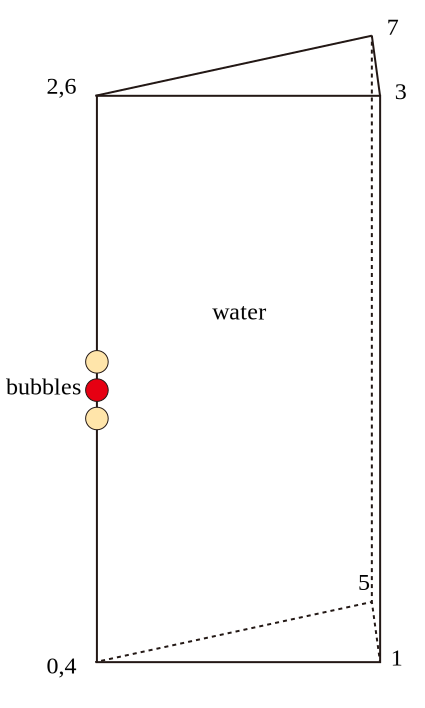
\includegraphics[width=0.45\linewidth]{img/fig4.14.pdf}
    \caption[楔形对称计算域。]{楔形对称计算域。点以数字方式标注。空泡以红色表示。在计算域中,(0,
2, 6, 4)设置为旋转对称面,底面(0, 1, 5, 4),顶面(2, 3, 7,
6),外面(1, 3, 7, 5)属性是 patch,前后面(0, 1, 3, 2)、(4, 5, 7,
6)是对称面 wedge。}
    \label{fig:4.14}
\end{figure}

在本章前几节中,实验研究了激光空泡间的相互作用,其呈现出特殊的膨胀和收缩形态。实验中给出的五种典型案例,表现出了不同的膨胀和溃灭机制。我们将这些机制总结为空泡间的抑制作用与初始距离限制的竞争。在距离较远时的弱相互作用,空泡间的推动作用较小而吸引作用较为明显。继而在收缩阶段产生向中心聚集的效果。在间隔距离次远时,空泡间形成一定的拉伸效果,并使空泡的寿命延长。在间隔距离等于两个相互孤立空泡半径和时,在收缩阶段形成较为明显的拉伸效果,并使中心位置的空泡在溃灭时形成较为明显的长条状。在距离更小时,拉伸效果非常明显,存在将中心位置空泡拉断的情况。但在距离足够小时,距离的作用压制了膨胀的推动作用,使空泡的膨胀和收缩都被压制。形成近似空泡合并的效果。
在这些不同机制的相互变化过程中,可能存在着某种突变或者渐变机制。为了更加详细、明确和物理地探究距离对这种线性排列的空泡间相互作用的机制,本节中借助模拟计算,对该问题进行参数研究。也就是$\gamma$以0.1:0.1:2的方式形成20组结果对比。
数值模拟采用如第二章第五节中给出的基于OpenFOAM的算法实现,并对本章中涉及到的案例做如下特殊设置。

在 OpenFOAM
中,通过单层三维网格获得二维网格模式。在本例中,设置为楔形结构,如图
\ref{fig:4.14}所示。其中地面和顶面以及外面三个面设置边界为:压力,''waveTransmissive'',无反射边界;速度,''pressureInletOutletVelocity'',流入流出边界。如此设置可以获得近似自由域的效果。但为了更好的对实验结果进行解析,基于传统的模拟求解设置,也就是计算域的边界距离空泡中心
$20 R_\mathrm{max}$ 以上。这里设置为 $25 R_\mathrm{max}$
,同时也是实验中容器的大小。本节中设置的情景并不完全对应于实验结果,而是更理想化的自由域情景,比如实验中存在水域的硬边界和软边界,在本节中统一设置为自由域边界。
本节构造了如图 \ref{fig:4.15}
的计算域。为了减少计算时间和提高计算精度,空泡区域的网格密度设置较高,并构成阶梯形式减少的正方形(六面体)结构化网格。在初始生成的计算域中,空泡计算域的网格密度为
$X*Y=(250/5\,\mathrm{mm})*(250/5\,\mathrm{mm})=50*50\,\mathrm{(mm}^{-1})^2$。

\begin{figure}[H]
    \centering
    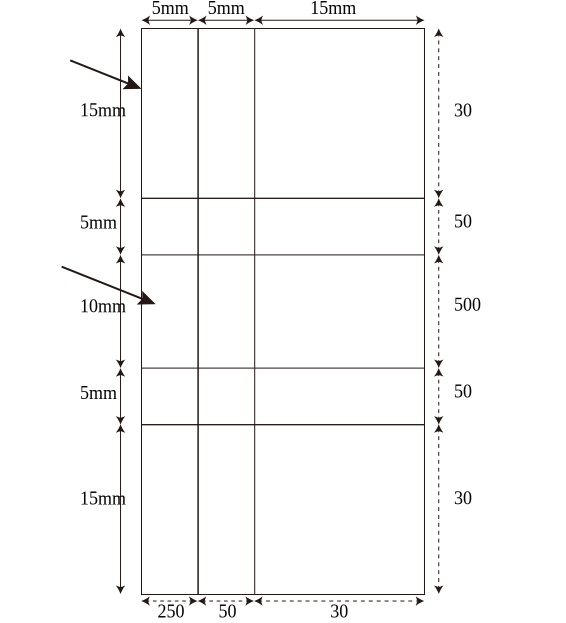
\includegraphics[width=0.5\linewidth]{img/fig4.15.pdf}
    \caption[二维网格划分正面图。]{二维网格划分正面图。计算域尺寸标注在左侧与顶部。对应尺寸划分网格数量标注在右侧和底部。从而获得在图中空泡区域均匀的
0.02mm 网格尺寸。}
    \label{fig:4.15}
\end{figure}


而空泡区域的网格尺寸 $20\,\mathrm{\mu m}$ ,
相比空泡的最小泡半径(初始泡半径
$34\,\mathrm{\mu m}$)处于同一数量级。这不足以精确的追踪空泡的脉动。通常要求最小泡半径时有\textasciitilde100
左右个网格。本文中采取更加极端的选择,即在空泡的脉动区域形成更小的网格尺寸。为此针对空泡区域做了四次网格细化,每次细化将
$X$ 和 $Y$ 方向上 2
倍密度,也就是一个正方形网格变成四个正方形网格。具体到不同 $\gamma$
值,则如图 \ref{fig:4.16} 中所示,形成四次细化。最核心部分的网格密度可以达到
$X*Y=50*50\,\mathrm{(mm}^{-1})^2*(2*2*2*2)^2=800*800\,\mathrm{(mm}^{-1})^2$。也就是最小网格尺寸为
$1.25\,\mathrm{\mu m}<1/20*R_\mathrm{init}=1.7\,\mathrm{\mu m}$。如此的设置后,不同的
$\gamma$
案例,其网格总数量不太一致,但总体每个计算域有\textasciitilde{}
$2\times 10^6$ 个单元格。

\begin{figure}[H]
    \centering
    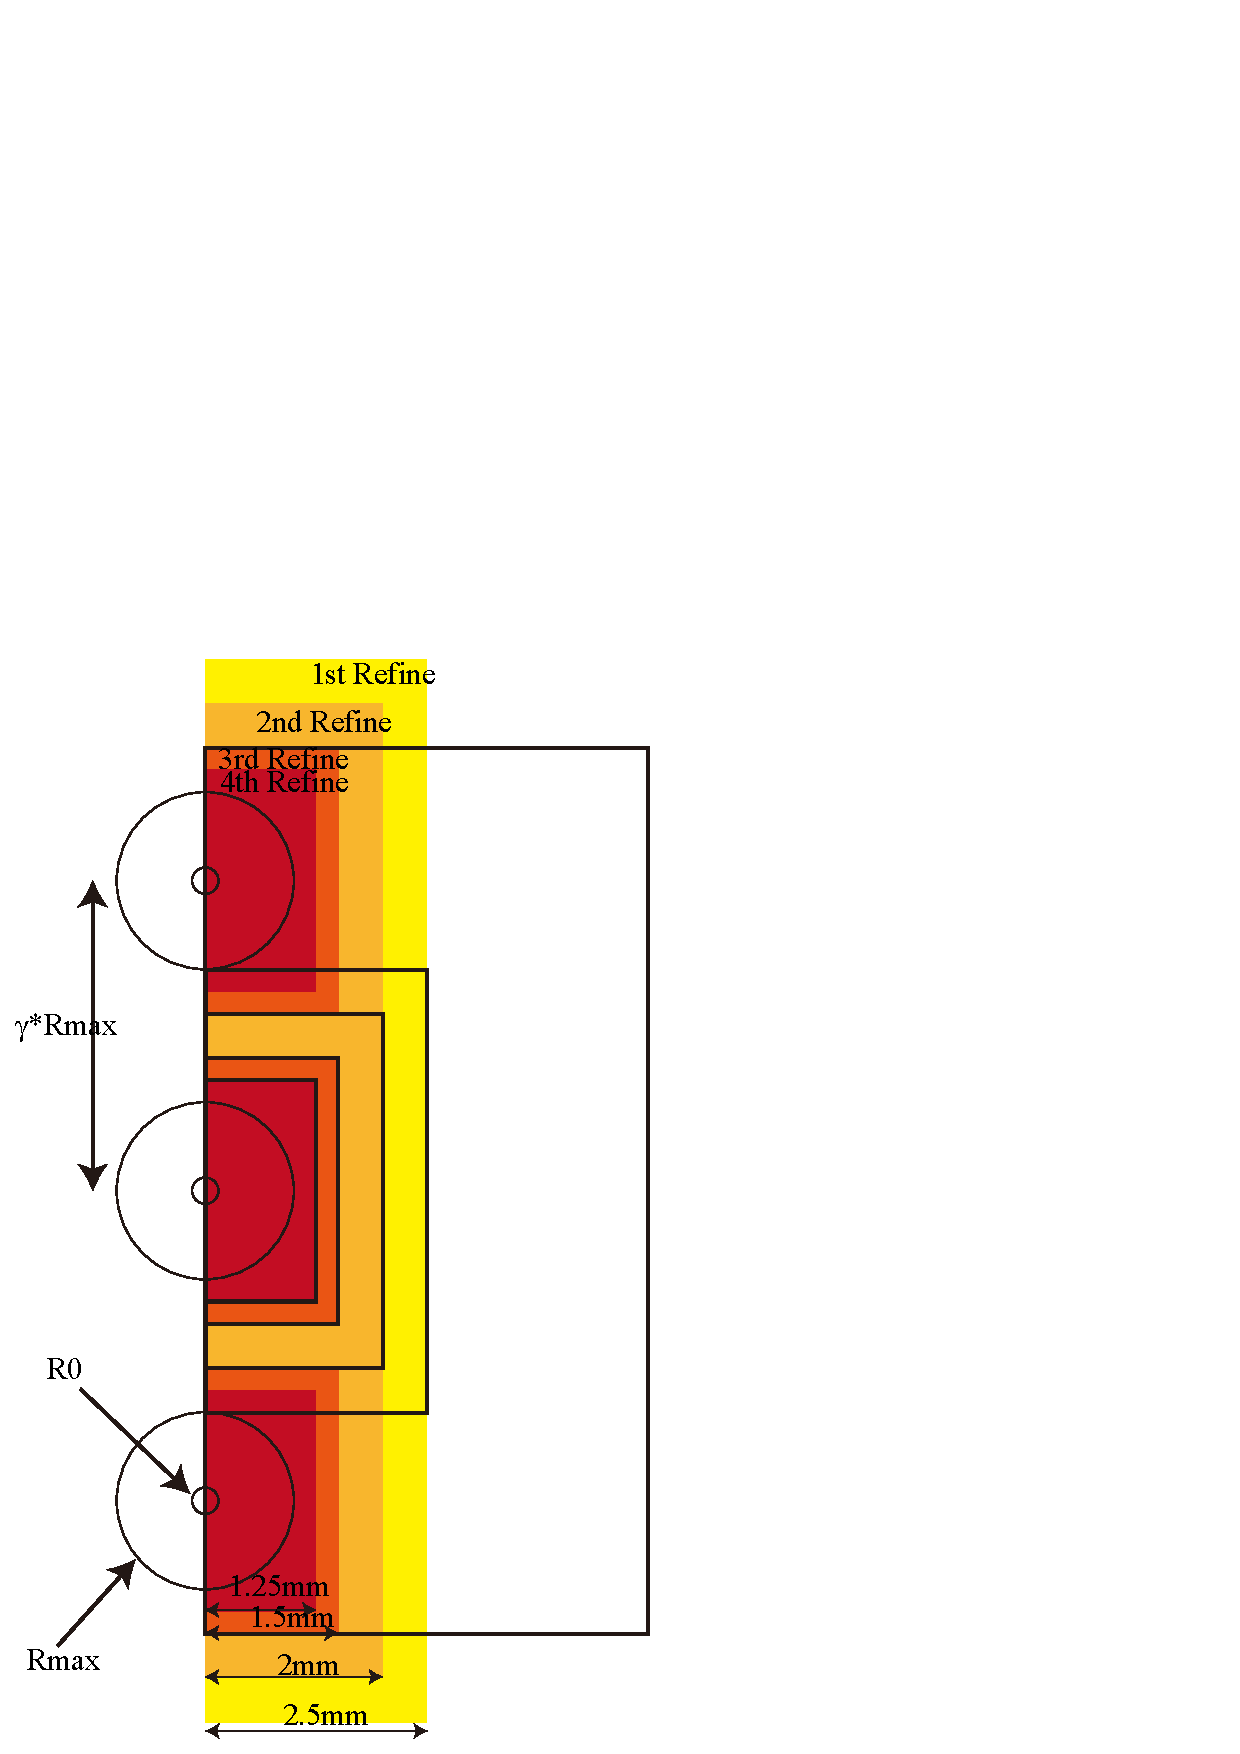
\includegraphics[width=0.6\linewidth]{img/fig4.16.pdf}
    \caption[]{对图中空泡区域的细化,如图中所示。细化顺序由颜色从浅至深标注。其中第一次细化范围是每个空泡中心的
2.5mm 边长的正方形,第二次细化 2mm,第三次细化 1.5mm,第四次细化
1.25mm。在相同的细化过程中,如果三个空泡周围的细化范围有所重叠,则细化范围取其范围并集。}
    \label{fig:4.16}
\end{figure}


\subsection{线性对称排列的三空泡的仿真}
上述的 20
组模拟中,模拟结果表现出较好的规律性,也揭示了一些实验难以获得的信息。上文中实验给出的五组
$\gamma$ 值,其对应的模拟结果相云图如图 \ref{fig:4.17}所示。

\begin{figure}[H]
    \centering
    \includegraphics[width=0.8\linewidth]{img/fig4.17.png}
    \caption[模拟的线性对称排列的三空泡气相云图]{模拟的线性对称排列的三空泡气相云图。通过计算域对其对称轴对称获得。}
    \label{fig:4.17}
\end{figure}


在如上图所示的模拟结果中,较好的获得了空泡间相互作用的过程。与实验结果类似,模拟获得的三空泡阵列膨胀收缩过程中的拉伸和挤压效果突出。通过二维计算所展现的结果,需要绕对称轴旋转才能展现实验中获得的阴影效果。

模拟结果中,对现象的解释此处与上文相符,不再赘述。
在实验中我们根据空泡在溃灭后的破碎残余气体团,推断空泡之间存在着一定程度上的间隔,并据此将空泡分割。在模拟结果中,我们可以观察到,空泡在膨胀期间其水膜稳定存在,但在收缩期间,取决于
$\gamma$
值,水膜过薄时会因拉伸效应和张力的共同作用使水膜断裂成间断排列在原水膜位置上的小液滴。通常这种现象被称为接合(coalescence)。在上述的模拟结果中,这种现象发生在
$\gamma\leq 0.6$
情景下的收缩期间。水膜断裂时通常会在空泡边缘形成凹陷,这是空泡接触所形成的特殊结构,我们仍然可以拓扑的分辨各个空泡的主体。特别地,在
$\gamma\leq 0.4$
时,因空泡间距过近,空泡在膨胀阶段就挤压水膜形成断裂,在最大半径时就完成接合。如此三空泡表现为近异形单空泡的脉动。
另外值得关注的问题是中间空泡的溃灭方式。在线性对称排列的三空泡中,边缘空泡的溃灭方式相互类似,同时也类似于近壁面空泡溃灭,也就是产生自近自由面指向近受约束面的射流导致溃灭。在实验中,我们基于现有的实验结果,以及对空泡控制的不确定性,认为主导中间空泡形成三种溃灭方式的主要原因在于边缘空泡的挤压作用与拉伸作用的斗争。这点是基于学界现有认知和有限的实验结果所获得的科学结论。但在模拟中,因条件的设置更加理想化,使结果中另一种特殊的可能存在的机制暴露出来。也就是在上文的讨论中提到的,在中间空泡收缩过程中,因自身收缩形成射流,或边缘空泡的射流刺穿边缘空泡后进入中间空泡。在相对方向前进的射流,在接近中间空泡的中心位置处相互撞击后,向射流发展的正交的方向延展,在空泡形成自内而外的水相体,使中间空泡自中间层断裂,形成类似拉断的效果。

上一节中提出的三种中间空泡的溃灭机制:1. 拉长; 2. 拉断;3.
上下挤压。其中 2.
拉断合并了上述射流撞击机制可以为断裂机制。针对这三种机制(拉长,断裂,挤压),选取其代表案例的压力和速度场的云图如图
4.18 所示。

\begin{figure}[H]
    \centering
  
    \subfigure[]{
    \includegraphics[width=0.3\linewidth]
    {img/fig4.18a.png}
    
    }
    \subfigure[]{
    \includegraphics[width=0.3\linewidth]
    {img/fig4.18b.png}
    
    }
    \subfigure[]{
    \includegraphics[width=0.3\linewidth]
    {img/fig4.18c.png}
    }
    \caption[三种空泡溃灭机制的压强-相态-速度云图。]{三种空泡溃灭机制的压强-相态-速度云图。
A 显示了挤压机制,其对应 $\gamma=0.5$。图 4.18B
显示了断裂机制,其对应 $\gamma=0.9$。图 4.18C 显示了拉长机制,其对应
$\gamma=1.5$。}
    \label{fig:4.18}
\end{figure}


 在图 \ref{fig:4.18}~.A
中,第一帧显示了边缘空泡开始收缩,但中间空泡仍在膨胀期的压力-相-速度图。可以看到空泡在接触面处延展。第二帧显示了三个空泡都进入了收缩其时的状态,可以看到泡外水体较为均匀的流向空泡区域,并且在边缘空泡内部,主要与对称轴平行地流向空泡接触面。这也就造成了在后期形成碟状结构,即在空泡的主轴长度保持较高长度,而次轴形成溃灭。第三帧中,三个空泡继续收缩,但上述平行的运动趋势仍然存在。第四帧中边缘空泡的射流进入空泡阵列内部。第五帧射流撞击,并形成向外的内生水体,此时空泡内部压强仍小于环境压强,且水体速度仍指向空泡阵列。第六帧显示了如实验图中溃灭末期的景象,水体主要在空泡排列方向流向空泡内部,即挤压模式下的碟形溃灭。

在图\ref{fig:4.18}~.B
中,第一帧显示了射流形成并向阵列内运动的情景。此时中间泡的长度因为距离较大形成的空泡间适度拉伸而形成较大的长度。第二帧显示了三个空泡持续收缩,边缘空泡形成的射流指向中间空泡的内部。第三帧显示,相对射流进入中间空泡内部,中间空泡的外壁仍在收缩但射流附近形成向外的趋势。第四帧显示射流撞击并产生向外延展的水体。第五帧,射流持续撞击,内生外延水体撞击中间空泡外壁。第六帧中,在边缘空泡的牵拉和内生水体的共同作用下,中间空泡自中间破裂。也就是上述的断裂机制。

在简要的图 \ref{fig:4.18}~.C
中,第一帧展现了射流贯穿边缘空泡,中间空泡在被拉长的基础上收缩。中间空泡主要受正交于阵列排列方向的推动。第二帧中,边缘空泡的射流接触中间空泡,更强的流动促使中间空泡在正交方向上收缩。第三帧中中间空泡收缩到射流撞击前刻,可以看到速度达到了
250
m/s。第四帧中,空泡溃灭至极小,正交方向的水体与射流撞击,产生较高的本地压力可以达到
$5.8\times 10^7 Pa$。这种形成正交高速水体与边缘射流撞击的溃灭形式,就是上文中的拉长机制。

更宏观地,统计了 20 组不同 $\gamma$ 值的内外空泡的溃灭时间,以研究
$\gamma$
对内外空泡溃灭形式的影响。因为空泡的不对称溃灭,在空泡生存末期,不会有一个体积极小的瞬间,而是在射流刺穿后逐渐破碎,故而本文中将边缘空泡的射流到达相对面的瞬间作为空泡的溃灭时间,并将中间空泡的射流相对接触时当作空泡的溃灭时间。即空泡被液体贯穿(penetrated)的时刻当作空泡的溃灭时刻。而不是过度的追踪残余气体的脉动。
内外空泡的溃灭时间受 $\gamma$ 影响的曲线如图 \ref{fig:4.19} 所示。

\begin{figure}[H]
    \centering
    \includegraphics[width=0.8\linewidth]{img/fig4.19.png}
    \caption{不同间距条件下内外空泡被射流击穿的时间对比。}
    \label{fig:4.19}
\end{figure}


在图 \ref{fig:4.19}中,可以看到 $\gamma$
越小,也就是空泡间距越小,边缘空泡受其他空泡的影响越大,边缘空泡的溃灭时间越大。在图中,对应的孤立单空泡的生存时间是
$183\mathrm{\mu s}$,也就是无穷远处, $\gamma$
极大时,其溃灭时间会趋向于 $183\mathrm{\mu s}$。与之相反地,在
$\gamma \leq 1.2$ 时, $\gamma$
越大中间空泡溃灭时间越长。这是因为在这段区间,空泡间的拉伸效应将中间空泡持续拉伸,边缘空泡的射流进入中间空泡的路径增长,碰撞时间变长。同时因距离增大,中间空泡的膨胀时间更长,膨胀更加充分,也推迟了其溃灭时间。在
$\gamma>1.2$
时,因泡间相互作用减弱,拉伸效果也减弱,造成溃灭时间减小。特殊地,在
$\gamma \leq 0.6$ 时,空泡在溃灭阶段形成一个大的接合空泡,在
$\gamma \leq 0.4$
时空泡在膨胀阶段就接合成一个大空泡。在这个区间,空泡接合,一般的,间距越近,其相互作用越强越早,接合成一个大空泡的能量越高,持续的时间越久。

同时,为了量化的反映空泡溃灭机制,定义一个参数,空泡溃灭瞬间的长短轴比,
$$
\chi  =\frac B A  =\frac {Y_\mathrm{end}} {X_\mathrm{end}} 
$$
此处 $A$、$B$ 的定义如上文中给出,在模拟中,我们固定的将 $A$ 与
$X_\mathrm{end}$、$B$ 与 $Y_\mathrm{end}$ 等效,即模拟中空泡在 x-y
轴上的边界值就是主次轴长。$\chi<1$ 时,溃灭的形态偏挤压, $\chi>1$
时,溃灭的形态偏拉伸。下图中(图 4.20)给出了不同 $\gamma$
值下的中间空泡的 $\chi$ 值。

\begin{figure}[H]
    \centering
    \includegraphics[width=1\linewidth]{img/fig4.20.png}
    \caption[空泡溃灭时的长短轴。]{空泡溃灭时的长短轴。A
给出了分别在边缘或者中间空泡被穿刺时的中间空泡主次轴长比。B
则给出了对应的情景下的主次轴长度。}
    \label{fig:4.20}
\end{figure}


从图 \ref{fig:4.20}中可以看到, $\chi$ 在 $\gamma=1.4$ 时获得最大,也就是在
$\gamma=1.4$ 时获得最好的拉伸效果。在 $\gamma=0.9$ 时获得
$\chi\approx 1$ ,也就是其溃灭时主次轴比约为
1,具有较好的圆性,可以形成较强烈的溃灭效果。同时,可以发现,在
$\gamma>1.4$
时,溃灭时的主轴长度几乎不发生变化,由此可知在此情景下,无穷远处对空泡的影响趋同,泡间相互作用影响其拉伸效果。在
$\gamma<1.4$
时,因为泡间相互作用造成在泡间阵列排列位置上的挤压和正交方向上的延展,遗留到溃灭阶段形成其交叉形状。

\section{本章总结}

在本章,实验和数值研究了均匀分离的三个激光致空泡的动力学。实验中,利用光学全息法在三维准自由水域获得特定排布的多点激光击穿,并借此在水中获得击穿空泡。精密控制的距离和能量实现了较为理想化条件下的单生命周期内的多空泡的相互作用。$\gamma$
作为均匀分布的多空泡间距的参数,在本研究中作为主要研究参数。

1.在阵列空泡中,空泡的生存时间普遍延长,体积变小。这种现象因中间泡受到的抑制最明显而使中间泡最为突出。在溃灭时,这种生存时间差使空泡的溃灭从外到内有序进行。同时,$\gamma$越小这种现象越明显。

2.空泡的不同部位的不同相位延迟造成了空泡的特殊形状。以一种相对独立的视角来看,可以认为,一个空泡内部部分,距相邻空泡越近的部分其相位推迟越大。这种现象是通过空泡与空泡脉动的声辐射相互作用来实现。
声辐射使空泡内外压差产生变化,在相应的脉动阶段对继续运动产生抑制效果,从而使空泡产生的相位推迟。

3.同相位等间距的三空泡系统中,中间空泡的溃灭形态有多种:不受影响,稍微在排列方向上拉长,拉长至长条状,沙漏状,和被压缩的碟型。中间泡不产生射流,两边向中间射流并且随着
  $\gamma$
  值的减小而变得强烈。一般地表示空泡形状稳定性的参数------圆性的开始失去可以发生在任意阶段,并随着
  $\gamma$ 减小而向前移动,从溃灭末期直到初生阶段。


4.在空泡阵列脉动期间,空泡通过声辐射相互作用,泡能转移使相对位置变动。在膨胀期,边缘空泡被向外推动。在收缩期则牵拉边缘空泡向内移动。$\gamma$越小,这种效果越明显。

在本章中利用多个参数来描述空泡的相互作用。未来需要有更进一步的描述相互作用过程中形变的参数。需要对生命周期的延长进行量化。对空泡能量的去向有更准确的计量。同时要改进实验方法,以期获得更准确的相互作用中空泡内部的信息。

%
\chapter{激光致空泡与压力波相互作用动力学}\label{chapter5}

在本章中,将从实验和数值计算等角度探讨激光致空泡受不同的压力扰动的动力学机制。将着重对空泡在脉动过程中受到压力波扰动,和空泡出生在不同压力波相位的而受到压力波的影响。出于简化模型的考虑,在本章中,我们将压力波简化为正压部分和负压部分,亦即压力波和张力波的组合。这个压力波以在一定距离外的压力入口处输入正弦波获得。
\begin{figure}[H]
  \centering
  \includegraphics[width=0.5\linewidth]{img/fig5.1-eps-converted-to.pdf}
  \caption{空泡时间和压力波时间对比图。}
  \label{fig:5.1}
\end{figure}



在这里,我们关注空泡产生与压力波入射时间的时间差
$\Delta T =t_{\text{bubini}}-t_{\text{pulse}}$

我们定义一个无量纲变量,
$$\Delta \tilde{T} =\frac{t_{\text{bubini}}-t_{\text{pulse}}}{T_{\text{bubble}}}$$
此处, $t_{\text{bubble}}$
指空泡的出生时间,即激光击穿时间。$t_{\text{pulse}}$
指压力波前到达空泡位置的时间。而这两者的差即
$t_{\text{bubble}}-t_{\text{pulse}}$
为正时,压力波已经开始影响空泡位置,空泡产生在压力波的影响中。差为负时,指空泡产生并运动了一段时间后,压力波前到达空泡位置,并开始影响空泡脉动。
$T_{\text{bubble}}$指空泡的第一运动周期。这里通过这个空泡运动周期来规范化空泡诞生和压力波前到达空泡位置的时间差,这样$\Delta \tilde{T}$
表达了这个时间差与空泡第一脉动周期的相对尺度。$\Delta \tilde{T}<-1$时,压力波在空泡第一脉动周期结束后到达空泡。$-1<\Delta \tilde{T}<0$时,压力波在空泡第一脉动周期到达空泡,其中$-1<\Delta \tilde{T}<-0.6$压力波波影响空泡的溃灭过程,$-0.6<\Delta \tilde{T}<0.4$,压力波影响空泡的稳定阶段。$-0.4<\Delta \tilde{T}<0$压力波影响冲击波的膨胀阶段。$\Delta \tilde{T}>0$时,空泡诞生在压力波影响范围内。

同时,还存在一个压力波时间尺度与空泡生存时间的对比,即
$$\eta=\frac {T_\mathrm{bubble}}{T_\mathrm{posip}}$$ 其中
$T_\mathrm{posip}$
指压力波的正压时间跨度。如果压力波和击穿激光同时扰动空泡位置情景下,即
$\Delta T=0$,当 $\eta>1$ 时,空泡脉动会同时遭受正压和负压,
$\eta<1$ 时,空泡只在正压范围内运动。

本章分为两部分,分别从实验、和求解 K-M 方程的理论结果。


\section{撞击驱动的空泡运动}

如前文所述,撞击作为一种简单的冲击波产生方式有其独特的优势。本节采用第二章中介绍的试管撞击法产生冲击波。产生的高强度压力波沿着试管方向传播,经由界面反射回水体后形成舒张波。在这个压力波在水体中传播过程的不同阶段注入空泡,能够获得不同动力学反应。并运用高速摄影法获得其脉动机制。

\subsection{撞击压力波与激光空泡相互作用的高速摄像系统实现}

为了研究激光致空泡在自由落体和压力波作用下的复杂环境内的脉动,设计的实验安排如图\ref{fig:5.2} 所示。内径 13.5mm 的试管装了 150mm
深的除气去离子水,并在试管轴处击穿形成空泡。由于试管的圆柱形状不利于光学观察和激光聚焦,采用高透玻璃做透光面的棱柱形外围容器包裹,并充满水,以实现光学折射率匹配。这个容器放在一个导引轨道中,以使试管撞击底部铝镁合金平板于同一位置。一束
He-Ne 红光用来以光门方式触发光电二极管(DET10A2,
Thorlabs)和示波器。当试管通过并遮挡住光波路径,延迟发生器(BNC525,
Berkeley Nucleonics
Corporation)产生一系列外触发信号。而空泡通过激光脉冲(Q2, Quantum Light
Instruments, wavelength 532 nm, 6 ns
duration)聚焦到试管轴上产生。空泡动力学过程通过高速摄像机((Mini AX
200,
Photron)获得。另外一个光电二极管用来记录等离子体闪光。拍照视野通过散射匀光的
LED 灯(SugarCUBE, Edmund
Optics)照明。通过高速摄像机拍摄的系列图像,可以获得空泡的等效半径
$R(t)$,即计算截面气相面积,并推导同等面积情况下的圆半径,以之为空泡的半径
$R(t)$。而为了通过图像获得空泡截面面积,首先平均阈值二值化,并以
$2*2$ 像素的正方形开运算并闭运算来移除噪音。

\begin{figure}[H]
  \centering
  \includegraphics[width=0.8\linewidth]{img/fig5.2-eps-converted-to.pdf}
  \caption[本章的实验设置]{本章的实验设置。a)
是实验装置的侧视图,b)
是俯视图。激光、高速摄像机、和传感器连接并通过示波器和延迟发生器(BNC525)控制。试管在导引结构内下落,并逐渐阻挡光电二极管的光门。BNC525
由此产生触发信号到激光器和摄像机。随后光学击穿产生空泡。空泡的产生时间通过另外的光电二极管受等离子体闪光触发所获得。试管撞击到平台,并随后产生向试管内传播的压力波。摄像机记录整个过程(帧率
160000fps,曝光时间 1/900000 s,视野 $128*128\text{pixels}^2$)。}
  \label{fig:5.2}
\end{figure}

试管在距离金属板 50mm
处释放,并在本作中所有涉及到的撞击实验中保持这个固定距离。如此,如图 \ref{fig:5.3}
所示在试管撞击到平台后,一个压力脉冲产生并在试管内通过水体向上传播。其在声学软表面------液气界面发生反射,由此产生的舒张波向下回传到空泡产生位置。

\begin{figure}[H]
  \centering
  \includegraphics[width=0.6\linewidth]{img/fig5.3-eps-converted-to.pdf}
  \caption[压力波在试管内产生和传播的时序图]{压力波在试管内产生和传播的时序图。T1 到 T4
表示时间时间顺序。试管在撞击平台 (T2) 前自由降落
(T1)。撞击产生了一个压力波向上传播 (T3),并经过激光聚焦 (T1)
产生空泡的位置。经过水气界面反射后,压力波反射会水体内行成张力波 (T4)。
t =0 表示压力波波前第一次到达击穿位置的时刻。激光在 $t=-\Delta T$
时聚焦到距离平台 25mm 处。在研究关注的时间范围内,空泡不发生较大位移。}
  \label{fig:5.3}
\end{figure}


压力波波前经过空泡位置时刻与激光致空泡产生的时刻的时间差 $\Delta T$
可以控制在较大的范围内变化。为了精准的获得撞击时间,将一个压电陶瓷压力传感器(SMD05T04R411,
STEMINC)粘贴到金属平台靠近撞击点的位置。并将一个针状水听器(Müller-Platte)布置到空泡产生位置。通过无激光入射情况下,同高度释放撞击,并记录压电陶瓷的脉冲时间与水听器的脉冲时间差,可以获得撞击后金属板上的弹性波脉冲波前到达压力传感器与水中压力波前到达水听器位置也就是后续空泡产生位置的时间差。在后续数据处理中,利用这个时间差以及压电陶瓷获得的压力信号,推算压力波波前到达空泡位置的时间。值得注意的是,水听器的接口不影响试管的自由落体,重复性的加载水听器或者卸载水听器的实验获得相似的结果。一个典型的水听器波形记录如图
\ref{fig:5.4} 所示。

\begin{figure}[H]
  \centering
  \includegraphics[width=0.6\linewidth]{img/fig5.4.png}
  \caption[冲击压力波,$p_i$,在未射入激光情况下原击穿位置测得(十次平均)]{冲击压力波,$p_i$,在未射入激光情况下原击穿位置测得(十次平均)。压缩相用红色标识,舒张相(反射导致)用蓝色标识。}
  \label{fig:5.4}
\end{figure}

从波形中可以看到,撞击后产生的压力波,传播到空泡位置的压力最高可以 8bar
左右。由于撞击压力的衰减和自由水气界面的反射形成的张力波作用,在 150
$\mu$ s 左右开始下降,并在 263.8 $\mu$ s
处下降到静压以下。压力舒张一直持续到 932.5 $\mu$ s。
除了撞击外,激光击穿同时也产生一个瞬态的压力脉冲。为了区分并考虑这两个压力源,分别记录了在无激光情况下撞击和无撞击情况下的激光击穿的压力波形。图\ref{fig:5.5}
显示了只有激光击穿压力情况的水听器压力记录。此时试管静止的放在平台上,而水听器放在击穿点正上方2mm处。该波形记录了空泡击穿冲击波信号,该击穿冲击波的反射波,以及空泡溃灭冲击波。从图中的击穿冲击波到溃灭冲击波的时间间隔测得的空泡生存时间约97 $\mu$ s。冲击波在 2mm范围内的速度较本地声速快,但这里将其处理成声速,形成的时间误差远小于空泡生存时间,故而忽略这个差别。

\begin{figure}[H]
  \centering
  \includegraphics[width=0.8\linewidth]{img/fig5.5-eps-converted-to.pdf}
  \caption[激光击穿冲击波压力]{激光击穿冲击波压力,在无冲击情况下的静态试管中,激光击穿位置上方 2mm
处测得的压力。}
  \label{fig:5.5}
\end{figure}

撞击产生的压力波与图 \ref{fig:5.5}
中显示的反射冲击波将在后续中结合,以重建空泡位置的压力。这是因为以现在的条件水听器不能直接放置在激光击穿位置并获得空泡遭受的压力,并且越靠近击穿位置,空泡将与水听器发生更加强烈的相互作用。如此,为了将实验与
Keller-Miksis 模型相比较,我们需要对空泡位置压力做一个更好的物理预估。
在降落和撞击实验中,空泡在其位置上遭受的压力 $p(t)$
可以看成两个压力的叠加,撞击产生的压力波 $p_i$
和激光击穿冲击波的反射波 $p_s$,即
$p (t)= p_i(t)+ p_s(t)$。通过有限元法(COMSOL
Multiphysics)模拟计算获得,空泡位置处收到的压力与 2mm
处压力相差不超过一个数量级。通过与实验结果的拟合(最小方差法),获得最佳重建压力比例系数为
k=8.3。即,可以将 2mm 处测得的反射波压力乘以
k,并添加时延后获得重建的空泡所受的压力,$p_s (t)=k p_\mathrm{hyd}^\mathrm{2mm}(t+\Delta t)$
。后续针对实验的数值计算中,使用这个压力当作空泡的驱动声压。

\begin{figure}[H]
  \centering
  \includegraphics[width=1\linewidth]{img/fig5.6.png}
  \caption{comsol
模拟获得压力重建乘数 k。}
  \label{fig:5.6}
\end{figure}

\begin{figure}[H]
  \centering
  \includegraphics[width=0.6\linewidth]{img/fig5.7.png}
  \caption[利用 2mm
处测得的压力(上)重建空泡处(下)压力]{利用 2mm
处测得的压力(上)重建空泡处(下)压力。重建压力在反射波到达前设置为
0。在受到影响后为
$p_s (t)=k p_\mathrm{hyd}^\mathrm{2mm}(t+\Delta t)$。并截至到 38
$\mu$ s,其后使用测得压力,并在空泡溃灭冲击波处后再次设置为 0。}
  \label{fig:5.7}
\end{figure}

\begin{figure}[H]
  \centering
  \includegraphics[width=0.7\linewidth]{img/fig5.8.png}
  \caption[利用重建的压力代入
Keller-Miksis
模型计算获得的空泡半径与使用其他压力的对比]{利用重建的压力代入
Keller-Miksis
模型计算获得的空泡半径与使用其他压力的对比。实验半径采自静止试管实验。模型计算的初值为
$R (t = 0) = 54.5\,\mathrm{mm}$,重建压力案例的初始速度为 1280
m/s,直接使用 2mm 水听器压力的案例初始速度为 540
m/s,使用静压条件的案例初始速度为 260m/s。所有案例在 94 $\mu$ s
左右处溃灭。均衡半径取自静止实验中 1ms 时,残余气体形成的小空泡
$R_0=0.09$mm。}
  \label{fig:5.8}
\end{figure}
在后续实验中,水听器放置在击穿点上方 10mm,以检测系列实验中的压力。


\subsection{静止和自由落体中空泡脉动的对比}

在特定高度释放试管后,试管内液体在试管撞击金属板处于失重状态。此时击穿水体形成空泡,空泡处于一个零加速度场中。

图\ref{fig:5.9}
上行显示了激光产生的空泡在无干预情况下,也就是试管静止时的动力学过程。它在本章中作为一个与自由落体和撞击情况的参照存在。在所有实验中,
$t=0$ 是激光击穿形成闪光的时刻,此时当作空泡的开始。在空泡形成后,其在
$t \approx 39.9\,\mu s$ 时能达到最大泡半径约为
$R_\textrm{max}=0.69\,mm$,并在 $t=96.1\,\mu \mathrm{s}$
时溃灭。因为试管体积的限制,这使得空泡的膨胀相和收缩相不再对称,这与在准自由场(即空泡距离边界
$20*R_{\text{max}}$
以上)中产生的空泡存在差别。这种现象可以用激光击穿冲击波及其后续反射波对膨胀相空泡的影响来解释。当空泡产生在立方体水箱中时,击穿冲击波因平面反射的缘故,不会在空泡位置产生汇聚效应,所以通常在水箱实验中忽略这种聚焦效应。但在此处实验中,因空泡产生在具有圆形界面的试管中央,击穿冲击波部分被试管玻璃壁面反射回空泡位置,从而影响空泡脉动。而冲击波产生到返回的时间大约是
$10\,\mu$
s,此时空泡处于膨胀相,使得空泡的膨胀现象受到明显抑制,具体推导见第二章实验设置。但相较于撞击产生的高强度,长持续时间的压力脉冲,这个聚焦冲击波对空泡的影响只有短时的压缩效果,对空泡整体上的膨胀和收缩过程的影响远远小于撞击冲击波。并不影响我们使用这种手段来研究撞击冲击波对空泡的作用机制。

在空泡溃灭后,空泡回弹,并在约 $t=139.9\,\mu \mathrm{s}$
时到达二次脉动的最大泡半径 $R_\textrm{max2}=0.43\,\mathrm{mm}$
,然后再次在 $t=164.9\,\mu \mathrm{s}$
时溃灭。这之后,空泡仍然持续脉动,直到泡能消耗。这个过程约持续到
$t=400\,\mu \mathrm{s}$ ,并因浮力作用而逐渐上浮,离开空泡原位置。图\ref{fig:5.9}
所示的两例空泡脉动半径曲线图在图 \ref{fig:5.12} 中显示为黑色和红色的点。

图\ref{fig:5.9} 
底行自由落体案例的空泡脉动的动力学过程。此自由落体案例是指,在特定高度释放试管后,射入激光产生空泡,空泡在试管撞击金属平面前的后续脉动过程。空泡在自由落体和静止状态下的动力学表现非常相似。
图 \ref{fig:5.10}
也显示两种不同帧率拍摄下获得的空泡半径随时间变化的曲线。cut-method
是将高速摄像取较小的分辨率($8*128$)以获得较高的帧率,而只拍摄到如切片一般的空泡中心区域阴影的方法。试管的微位移造成的空泡位置变动是
cut-method
测得空泡半径变化的主要因素。多次采样间的激光能量密度,和试管微位移造成的击穿冲击波及其后续压力波变化,是影响多次测量间不同结果的主要因素。
针对自由落体和静止状态案例,我们认为在空泡尺寸不够大的情况下,重力的影响十分微弱。在第三章中给出的参数$\zeta=-\rho g R_{\text {max}} \Delta p^{-1}$,可以间接的用来表达空泡形变的程度。在实验案例中,设定最大泡半径为
$R_\textrm{max}=0.7\,$mm,环境压强 $p_a=1\,$bar ,获得的
$\zeta= 7\,*10^{-5}$,远远小于能够产生微射流的阈值$\zeta = 10^{-3}$。这也证明在百微米和毫米尺寸的空泡完全可以忽略重力的作用。

\begin{figure}[H]
  \centering
  \includegraphics[width=1\linewidth]{img/fig5.9.png}
  \caption[静态和自由落体环境下的空泡动力学过程的照片]{静态和自由落体环境下的空泡动力学过程的照片。每一帧照片对应的时间标注在图片上方。上下栏分别对应了静态和自由落体的案例。标尺标注于于下栏的末端。激光自每帧图片的右方射入,而撞击产生的压力波垂直的自下而上传播。
}
  \label{fig:5.9}
\end{figure}




\begin{figure}[H]
  \centering
  \includegraphics[width=0.7\linewidth]{img/fig5.10-eps-converted-to.pdf}
  \caption[两种方法测得的空泡半径对比]{将相机图像中心稳定到空泡初生位置,分别采用大帧率小视野(cut
method)、和大视野小帧率两种方法获得空泡的半径。前者使用最远距离为空泡直径,后者使用面积法获得半径。误差由十次采样的平均方差表示。
}
  \label{fig:5.10}
\end{figure}




\subsection{瞬态压强驱动的空泡及空泡团簇的运动}

图\ref{fig:5.11}
是显示了在不射入激光的情况下,试管自由下降并撞击金属平台,在空泡产生位置测量得的撞击压力波。正压力波持续了
$263\,\mu$ s,随后进入舒张波阶段。舒张波持续到 $t=932\,\mu$
s。并继之一些后续波动。在整个压力波阶段,正压可以达到 $8\,$
bar,而负压能达到 $-5.5\,bar$ 。

本节将讨论四种不同空泡产生时间相位下的空泡动力学。空泡的产生如图 \ref{fig:5.11}. b
所示。''L''代表激光入射时间。静态情况下,空泡的第一脉动周期持续
$96\,\mu$ s,小于在脉冲压力的正向周期。
四种情况分别是:(a)空泡先于压力脉冲产生;(b)空泡在脉冲正压的波峰附近产生;(c)空泡先于负压开始产生;(d)空泡在负压中产生。此四种情况在图\ref{fig:5.11}
中显示。对应的实验图的时序也标识在该图中。

\begin{figure}[H]
  \centering
  \includegraphics[width=1\linewidth]{img/fig5.11.png}
  \caption[压力波形与照片对应图]{ a) 即图\ref{fig:5.2} 压力波形图。b) 图 \ref{fig:5.13}
中图的时间线。每帧用空心菱形$\diamond$标注。绿色实心菱形并以``L''标注的是该案例的激光入射时间。}
  \label{fig:5.11}
\end{figure}



\begin{figure}[H]
  \centering
  \includegraphics[width=1\linewidth]{img/fig5.12.pdf}
  \caption[典型案例的空泡半径-时间曲线图]{典型案例的空泡半径-时间曲线图。实验数据以符号图表示,而使用
Keller-Miksis
模型计算所得的半径使用实线表示。此处的半径是指等效半径$R (\text{t})$,即根据面积求得等面积圆形的半径。图中所包含的六种情形对应图
\ref{fig:5.9} 和图 \ref{fig:5.13}。误差棒表示了图像处理所致的不确定度。b)与
a)同样的实验,但延长其时间尺度到包含了后续空化云动力学过程。
}
  \label{fig:5.12}
\end{figure}



\begin{figure}[H]
  \centering
  \includegraphics[width=1\linewidth]{img/fig5.13.png}
  \caption[产生于四种不同的压力波相位的空泡和空泡团簇动力学过程照片]{产生于四种不同的压力波相位的空泡和空泡团簇动力学过程照片。每一排以激光射入时的压力波相位区分,相位则用时间延迟
$\Delta T$
表示,也就是激光空泡产生时间减去压力波到达空泡位置的时间。压力脉冲在图
\ref{fig:5.11} a 中展现,对应的空泡半径演化在图 \ref{fig:5.12} 中展现。蓝色 $t (p-)$
标记显示了在空泡时间线上,每个案例中空泡所遭受的环境压力变为负压的时间点。每个案例的最后一帧标记了标尺。案例a),
$\Delta T=-50.2\,\mu \mathrm{s}$,显示了空泡在压力波到达之前产生,并在第一个脉动周期受影响的情况。案例b),
$\Delta T=77.8\,\mu \mathrm{s}$,显示了空泡在高压阶段产生的情景。案例c),
$\Delta T=238.6\,\mu \mathrm{s}$,显示了空泡产生在环境压从正压到负压的转换点附近的情景。
案例d),
$\Delta T=267.3\,\mu \mathrm{s}$,显示了空泡在负压阶段产生的情景。}
  \label{fig:5.13}
\end{figure}

在图 \ref{fig:5.13}中显示了四种不同脉冲相位产生的空泡。 图 \ref{fig:5.13}. a
显示了压力脉冲在空泡处于最大泡半径阶段时开始作用于空泡的情景。此种情形下,在竖直方向上存在压力梯度。高压加速了空泡的溃灭,继而减少了空泡的生存时间,见图
\ref{fig:5.12} 的 $R(t)$ 曲线。空泡的回弹也因为高压压迫而形成较小的空泡半径。在
$t=89.2\,\mu$ s,如图 \ref{fig:5.13}a
中箭头所示,可见清晰的逆重力方向,也就是顺着脉冲传播方向的射流形成。此射流的形成与压力脉冲的空间分布有关。我们使用如第三章中介绍的各向异性参数
${\zeta}=\left|\nabla p\right| R_{\text{max}} \Delta p^{-1}$
来辅助解释这个效应。据图 \ref{fig:5.11}. a 的斜率,代入水中声速
$c=1483\,ms^{-1}$,我们可以估算
$\left| \nabla p\right| \approx 436\,$
bar/m。从而,在空泡第一次溃灭,射流形成时, ${\zeta} \approx 0.30$
。这样的梯度比冲击波驱动的空泡溃灭要小得多\cite{sankin_shock_2005}。从而,射流在空泡的再膨胀阶段
$t=89.2\,\mu$ s.才明显可见。空泡在 $t=126.7\,\mu$ s
附近发生第二次溃灭。后续在 $t=314\,\mu$ s
张力波射入时,微小的空泡溃灭后残余混合气团,膨胀成为一群大空泡团簇。这群团簇持续生存至大约
$t=1500\,\mu$ s。

图 \ref{fig:5.13}.b 展现了空泡在正压相产生的时间序列照片(序列位置见图\ref{fig:5.12}.
b)。空泡在约 $t=9.5\,\mu$ s
时到达最大泡半径。而这个最大泡半径远远小于参照组的最大泡半径,即静压案例的
$R=0.69\,mm$。而且该情况下,高压而大大减小了空泡的生存时间,也大大减少了空泡后续脉动的持续时间和幅度。在这里,第一次溃灭时空泡在垂直方向上溃灭,由此形成水平排列的空泡碎片,这些碎片随着时间的推移而扩散。在溃灭过程中可能由于高压产生了一个水平流,运输空泡碎片。最后,空泡的残余混合气团在环境转为舒张相时,
$t=240.7\,\mu$ s
,被拉伸成为一群空泡团簇。这团空泡团簇,在溃灭时,因水平和竖直方向的相位差异,形成竖直方向的射流击穿空泡,并形成竖直分布的二次残余气团,如
$t=1441\mu$ s 所示。

在图 \ref{fig:5.13}. c
中,空泡产生于压力脉冲的正压相的终末阶段。此时,相比于参照组,其在产生和膨胀初期仍然受高压相的压迫,而使其最大半径及时间相应减小。而在空泡收缩时,由于环境压降低至舒张相,使空泡收缩收到抑制。继而没有产生溃灭,直接再膨胀。在再膨胀过程中(
$t>55\,\mu$
s),在空泡原位置的左右处产生了继发空泡。这是由于激光在当地传播过程中,电子密度不足以形成击穿,但是形成微小的体积相变。这些相变位置作为凝结核,在收到张力波作用后形成新的空化。由于这种激光和张力的双重作用,形成的随机空泡多数尺寸在分辨能力以下。但在激光路径高热区形成的这些空泡与原空泡碎片膨胀合并,在
$t=900\,\mu$ s 处达到最大泡半径,并在 $t=1300\,\mu$ s 时溃灭,参考图\ref{fig:5.12}
。

图 \ref{fig:5.13} 中,案例 a) 到 c) 都受到高压相影响,而案例 d)
则是空泡产生于张力相。张力持续了 $668\,\mu$ s
。在此期间空泡膨胀成为一个相比于静态空泡尺寸非常大的单体大体积空泡,即
$R_\mathrm{max}=2.22\,$ mm 与 $R_\mathrm{max}=0.7\,$ mm 对比。在
$t=932.5\,\mu$ s
时,压力重新转为正压,此时空泡开始收缩。空泡溃灭时是一个凸出的椭圆体,其次轴与重力方向一致。此处形状来源于叠加边界和压力波的双重作用。由于试管壁的存在,边界阻碍了水从侧面的流入补充空泡收缩让出的空间。后续正压在竖直方向上形成压力梯度,助长了这种形状。双重作用形成的压力梯度诱发了向上的喷射流,在图
\ref{fig:5.13}.d 中 $t=1544\,\mu$ s 处很明显。

除了实验数据,图 \ref{fig:5.12}
显示了数值模拟的各自半径。一般地,实验和数值曲线在第一次振荡中是相当一致的。可以观察到后续的差别,这主要是由于忽略了空泡到空泡团簇之间的破碎过程,以及从团簇到球形空泡的近似。同时液域的圆柱形封闭限制了实验中空泡的膨胀和收缩,这一点在这个简单的计算模型中没有考虑。


\subsection{空泡对压力波的相位响应}

图 \ref{fig:5.14}. a 和 \ref{fig:5.14}.b 分别显示了空泡对 $\Delta T$
的响应的实验和模拟结果,$\Delta T$
是空泡产生时刻和脉冲压力通过空泡点的时间差 $\Delta T$ 。其中,空泡半径
$R(t)$ 是用颜色编码的。对于 $\Delta T=0$
的阶段,空泡是在脉冲压力波到达激光焦点的时刻产生的。$\Delta T$
的负值指的是在压力波通过前产生的空泡。虚线表示压力波到达空泡位置的时间。因此,从这条线开始,经过一段时间后,发现一个蓝色的区域,表示各自的空泡压缩。然而,对于
$250\,\mu$ s 和 $200\,\mu$ s
之间的阶段,第一次和第二次膨胀发生在压力脉冲通过之前。因此,空泡动力学基本与
$\Delta T$
无关,这个阶段范围内的空泡显示出基本相同的动力学,例如,它们都在
$100\,\mu$ s 左右崩溃。然而,在压力波通过前 $100\,\mu$ s
产生的空泡的反弹却受到影响。在更接近压力波通过的地方产生的空泡,例如
$\Delta T>-50\,\mu$
s,显示出第一个空泡膨胀的强烈减弱,只有微小的反弹。对于
$\Delta T>100\,\mu$ s(图中右下角的 $t>140\,\mu$
s),由于稀疏波的通过,空泡再次膨胀。

\begin{figure}[H]
  \centering
  \includegraphics[width=1\linewidth]{img/fig5.14.pdf}
  \caption[空泡生成时间与冲击波射入时间差$\Delta T$对应的空泡半径$R (t)$演化]{空泡生成时间与冲击波射入时间差$\Delta T$对应的空泡半径$R (t)$演化。时间零点$t=0$
,指空泡诞生时间。竖直轴是空泡产生时延,$\Delta T$,此处负值指空泡先于压力波作用产生。红白间断线代表了压力波开始时间。a)
实验结果。 b) K-M 与测得压力波结合计算所得的空泡响应。
}
  \label{fig:5.14}
\end{figure}

现在让我们把测得的空泡响应与图\ref{fig:5.14}. b
中的模拟结果进行比较。对于所有的模拟,Keller-Miksis 模型的初始条件是
$R(t=0)=54\,\mu$ m 和 $\dot{R}(t=0)=1280\,$
m/s,平衡半径,即不可凝结的气体量,是 $R_n=90\,\mu$
m。详情请见本作第二章。总的来说,我们发现实验和球形空泡模型之间有良好的定性和定量的一致性。特别是,随着
$\Delta T$ 的增加,空泡生存时间的缩短被很好地再现了。另外,在图 \ref{fig:5.14}.b
中右下角区域的大 $\Delta T$ 和大 $t$
的空泡开始重新膨胀的现象在模拟中得到了证实。良好的一致性也证明了空泡成核和脉冲压力产生的实验是高度可重复的。

模拟和实验之间有一些差异,在反弹中可见。在实验中,这些反弹持续的时间约为20\%。这可能是由于与模拟相比,实验中的溃灭较弱。实验中较弱的溃灭通过声发射消散的能量较少。因此,更多的能量可用于再膨胀,空泡膨胀到一个更大的半径。模拟溃灭辐射更多能量的原因可能是由于理想绝热气体的热力学简化导致,但也有试管的封闭几何形状的原因,这在模拟中没有考虑到。试管的几何形状阻止了球形汇聚流,与较大的比色皿相比,可能会导致较小的液体速度。

\subsection{空泡团簇脉动的脉动行为}
在压力波实验中,我们看到,除了空泡溃灭的时间缩短外,当脉冲压力的稀疏波部分与激光诱导致空泡相互作用时,可以诱导产生大体积空泡和空泡团。

在这里,我们在图 \ref{fig:5.15} 中,更详细地分析大体积空泡和空泡团作为相位
$\Delta T$ 的函数的动力学,使之涵盖了与之前的图 \ref{fig:5.14}相比更多的
$\Delta T$ 和时间 $t$ 的范围。 图 \ref{fig:5.15}. a
显示了实验的半径时间数据,图\ref{fig:5.15}. b
显示了模拟的空泡动态。请注意两图中不同的色标范围。左上方的图 \ref{fig:5.15}.
a,即小 $\Delta T$ 和小 $t$,是对之前图 \ref{fig:5.14}. a
的再现。正压的开始用红色虚线表示,标记为 $p+$。图\ref{fig:5.15}
最突出的特征是在 $p-$ 线之后形成的大红球。它的最大值在张力阶段开始后约
$500\, \mu s$ 达到。在 $p+$ 和 $p-$
线之间的淡蓝色区域表示只有非常小的空泡或根本没有空泡可见。其中仍然有空化核存在,一旦舒张波到达就会膨胀成空泡。这个区域在图
\ref{fig:5.15}.a 中被称为
``空泡群'',因为这里有多个空泡膨胀并合并。这里绘制的等效半径必须被理解为一个近似的半径。它是通过整合高速帧中被空泡覆盖的像素区域而得到的。通过假设是一个单一的投影空泡这个面积被转换为等效半径。

形成空泡团的多空化核的起源是激光诱导的空化空泡在其第一次和以后的溃灭过程中形成的小空泡碎片。同时,形成的微观气体碎片,会因扩散以及溶解的原因而减小。但这个溶解时间比$p+$和$p-$之间的时间跨度要长得多,也就是说,一旦稀疏波到达,这些碎片就会作为空化核。

\begin{figure}[H]
  \centering
  \includegraphics[width=1\linewidth]{img/fig5.15a.pdf}
  \includegraphics[width=1\linewidth]{img/fig5.15b.pdf}
  \caption[实验和 K-M
模型计算结果比较。]{实验和 K-M
模型计算结果比较。与图 \ref{fig:5.14}
具有相同的轴内容设置,但具有更长的包括空泡团簇过程的时间尺度。a)
实验获得的$R (t)$。图 \ref{fig:5.13}中显示的典型案例在 y 轴上特殊标识。b)
Keller-Miksis 模型计算获得的空泡响应,脉动半径$R (t)$。K-M
模型获得了较大的空泡半径,图色标尺作了截止处理,以获得更好的对比效果。红白间断线代表了压力波到达空泡位置的零时刻。蓝白剪断线代表了压力波转化为张力波的时刻。黑白间断曲线勾勒出了空泡溃灭时刻,而白色虚线将图划分为空泡团簇区域和单空泡区域。}
  \label{fig:5.15}
\end{figure}

图中提出的四种情况的 $\Delta T$ 的阶段在图 \ref{fig:5.13}纵轴上标出。案例 a)
和案例 b) 呈现较早的溃灭和空泡碎片重新膨胀成团的结果,而案例 c) 和案例
d) 则显示为单个空泡的膨胀。情况
c)特别有趣,因为在这里,正压作用在空泡上的时间很短,不足以诱发完全崩溃,空泡在收缩一段时间后,在负压的作用下重新膨胀为一个大体积空泡。有趣的是,这个单一空泡的生存时间明显长于以稍短的阶段
$\Delta T$ 产生的空泡群。

当空泡完全在张力阶段引入时(见 $\Delta T\geq 263.8\,\mu$
s),空泡扩展为一个更大的单一空泡,具有更长的第一次振荡周期,在这里它被张力阶段的持续时间所限制。这一点通过增加相位
$\Delta T$
时第一次振荡持续时间的减少得到证实。从空泡群到大的单个空泡的过渡发生在情况
c) 周围,见图 \ref{fig:5.15}.a 中的水平虚线。

实验和数值数据显示了类似的定性行为,尽管数值模型只考虑了单一的球形空泡。在实验中,空泡团机制的溃灭时间被高估了。我们将此归因于试管边界的影响,限制了实验中空泡的膨胀。因此,空泡没有像模拟中那样膨胀,在模拟中它们也较晚崩溃。
然而,一般认为,模拟中的空泡膨胀了大约两到三倍,这将对应于至少两倍的溃灭时间。但在实验中,溃灭时间最多只缩短了20%。这可以解释为,在空泡与容器大小相近的受限几何形状中,空泡的生存时间也会延长\cite{quinto-su_cavitation_2009}。

空泡的最短生存时间存在于 $80\,\mu$ s $\,\le Δ T\le 160\,\mu$
s,此时其被减少到小于 $20\,\mu$
s。这一发现在模拟中得到了再现。然而,对于空泡团的溃灭,我们看到实验和模拟之间的一致性较差。在模拟中,图
\ref{fig:5.15}.b,在第一次大膨胀之后,所有的空泡都以同样的方式重新膨胀,只是被
$\Delta T$ 的相位转移了。在实验中,只有在 $150,\mu$ s 和 $300,\mu$
s 之间的 $\Delta T$
观察到相当大的再膨胀。这清楚地表明,用这个简单的模型只能在一定程度上模拟团簇的动态。另外,再膨胀在很大程度上是由空泡内容物含量决定的。该模型没有考虑到质量运输、冷凝和蒸发。这对主要含有水汽的空泡来说特别重要,因为这里就是这种情况
\cite{akhatov_collapse_2001}.。

当负压在第二个振荡周期开始时,甚至在溃灭的很晚阶段,脉冲压力波仍然压缩第一周期的空泡,反射的溃灭冲击波也能影响它的反弹,这在计算中都没有考虑。越来越大的负压直接使第二个循环的空泡反弹。这在实验和计算结果中都很清楚。

在正压相的最后阶段产生的空泡脉动有着逐渐增大的脉动周期。这是由于空泡初始环境压力的降逐渐降低而导致的。
同时,空泡溃灭和团簇重生的时间相交,也就是空泡团簇重生机制转变为空泡自身反弹机制发生在$\Delta T=234\,\mu s$左右,即空泡产生于正压的很晚阶段,其中空泡的第一周期时间小于静态第一振荡时间。

空泡不能达到其可实现的最大半径和生存时间,即使它在溃灭阶段内遭受负能量。
我们认为能量损失发生在空泡产生的初始阶段,这也是与空泡相互作用的急剧变化的正压冲力的阶段。脉冲释放了新生空泡的能量,使其最大半径变小,例如,在$\Delta T=234\mu s$的情况下,空泡最大半径在$20\mu s$时约为6mm。
在空泡生成的$30\mu s$后,它遭受了负压,但其仍在收缩,直到$80\mu s$。此处,$\Delta T=234\,\mu s$是一个分水岭,正如数值结果所显示的,在这之前,负压不能在空泡溃灭之前使其半径回升。其后,空泡会在其溃灭之前反弹。由于溃灭抵消了张力,空泡失去了能量,所以它的生存时间明显缩短,这在图像上显示为一个缺口。
正如前面提到的案例$\Delta T=238\,\mu s$所示,在这个阶段产生的空泡并没有达到静态的最大半径,在缓慢收缩后,它又反弹了。
由于不充分的溃灭,空泡的能量在开始重生的时候会有一点衰减。
在这种情况下,少许衰减的空泡能量加上高负压使得空泡半径变的更大。

在后期负压阶段产生的空泡,在张力波的拉伸作用下,直接膨胀到空泡簇的最大半径,而不经过任何收缩。
在这种情况下,空泡有更多的能量。
与以前的情况相比,它使泡群的最大半径更大,生存时间更长,如图中的凸起所示。
随着空泡产生的时间继续在压力波时间正方向上移动,空泡生存时间和最大半径减少。
这是由于环境压力在达到最大值之前越来越早地上升到最初的正常水平。

尽管如此,第二个振荡周期也发生在空泡群上。但由于残留的溃灭的空泡气体比较分散,由于大体积空泡有更多的能量产生更密集的现象,很难区分和计数代表分散的小空泡的像素。所记录的新的反弹团簇是由多种来源引起的,这里不作讨论。

\begin{figure}[H]
  \centering
  \includegraphics[width=1\linewidth]{img/fig5.16.pdf}
  \caption[使用 Keller-Miksis
模型与测量获得的压力波耦合计算的不同空泡诞生和压力波时延
$\Delta T$,情景下的空泡团簇脉动。]{使用 Keller-Miksis
模型与测量获得的压力波耦合计算的不同空泡诞生和压力波时延
$\Delta T$,情景下的空泡团簇脉动。在没有脉冲压力的情况下,空泡只在
100µs 左右扩展到大约 700µm(见∆T \textless{} -100µs
的曲线)。当空泡的引入在时间上与舒张波开始相吻合时,空泡膨胀获得最大半径,它在最大膨胀时可以达到
8 毫米以上。数值曲线高估了测量的空泡尺寸约 4
倍,我们将其归因于管壁的影响和由此产生的空泡的几何限制。}
  \label{fig:5.16}
\end{figure}




由张力波引起的空泡群或大体积空泡膨胀到最大半径,这是受管子的有限体积和张力波的双重影响。
K-M模型通常用来解释准自由域中的空泡行为,而在这项工作中,重生空泡的半径与管子半径相似,因此不是很准确。然而,我们发现计算和实验中的重生簇生存时间都在$1.3\,ms$左右。这是由管子的周围形状引起的,它延迟了膨胀和溃灭的过程。


\subsection{空泡溃灭致辐射冲击波}


与仅由恒定的环境压力驱动的溃灭相比,强制溃灭可能导致空泡的压缩增强。

在图 \ref{fig:5.17} 中,它显示了激光射入后不同 $\Delta T$ 情况下从 $0\,\mu s$
到 $200\,\mu s$
的压力云图。为了从数据中读取峰值压力,我们对记录的信号使用了 40 kHz
的高通滤波,以去除本底压力波。用箭头 A 标记的垂直高亮线,大约在
$7\,\mu s$
左右,是激光击穿冲击波在图中的表现。它到达水听器时,压力仍然很高,约为
3.5bar。

随后,在所有的情况下都存在这种崩溃冲击波的多次反射。箭头-B
指向第一个空泡崩溃冲击波的高亮带。在 $\Delta T<53\,\mu s$
的情况下,它位于 $104\,\mu s$ 左右。箭头 C
指向强制溃灭冲击波的高光曲线。由脉冲压力波引起的加速溃灭放大了溃灭冲击波。在高正压区,脉冲压力波和空泡残余物之间的进一步相互作用产生了许多后续的峰值,这主要是由容器的强化冲击波的反射引起的。在入射压力由正转负后,空泡在环境负压的作用下膨胀而没有溃灭,这被称为大空泡的产生,在上面的案例
c)中得到了说明。正如箭头-D 所指出的,在 $\Delta T=240\,\mu s$
之后,第一个空泡溃灭冲击波消失了。它合并到空泡团簇的溃灭冲击波中,这时被称为大空泡溃灭冲击波。

\begin{figure}[H]
  \centering
  \includegraphics[width=0.8\linewidth]{img/fig5.17.pdf}
  \caption[10mm 处测得的压力云图]{10mm 处测得的压力云图。箭头
A:激光击穿冲击波。箭头-B:未受干扰的第一次空泡溃灭的溃灭冲击波,即当空泡在被脉冲压力波击中之前就已经溃灭。箭头
C 显示的是被脉冲压力波增强的第一次溃灭冲击波。对于较小的
$\Delta T$,表现为向左凹陷弯曲的曲线,因为压缩压力较早地击中了空泡,减少了空泡的生存时间。最终它又向右弯曲,因为空泡的大小在张力阶段变大。箭头-D:显示了第一次溃灭冲击波的消失,而实质上在该处空泡溃灭转变成大空泡机制,溃灭冲击波来自大的空泡溃灭。由于反射作用,A、C
所代表的冲击波的反射波在图中出现了多次。}
  \label{fig:5.17}
\end{figure}




为了表征溃灭强度,我们研究了不同 $\Delta T$
情况下的第一次溃灭冲击波峰值。图 \ref{fig:5.18} 中显示了(第一次)溃灭峰压力随
$\Delta T$
的变化。它包含了没有外界影响的空泡溃灭阶段、由压力波强迫的空泡溃灭,以及拉伸后的大空泡溃灭。每个溃灭峰值压力都经过了用其各自的等离子体冲击波峰值压力实施的归一化处理。即
$p=p_\text{impulse-peak}/p_\text{shockwave-peak}$。为了从数据中读取峰值压力,我们对记录的信号使用了
40 kHz 的高通滤波,以去除本底压力波。

空泡的生存时间显示为红色。空泡生存时间是击穿冲击波和溃灭冲击波两个峰值之间的时间差。蓝色曲线(第一次溃灭冲击波的峰值压力)的最大值在
$\Delta T\approx -30\,\mu$ s
附近。这一事实表明,当空泡在大部分时间在大气压力下膨胀,并且在空泡开始收缩时刻附近,瞬时压力波开始作用于空泡,此时空泡能够获得最强的溃灭增强(见图
\ref{fig:5.11} 中的波形)。

\begin{figure}[H]
  \centering
  \includegraphics[width=1\linewidth]{img/fig5.18.pdf}
  \caption[第一个溃灭冲击波的峰值压力(蓝色)和空泡生存时间(红色)关于
$\Delta T$
的演化曲线]{第一个溃灭冲击波的峰值压力(蓝色)和空泡生存时间(红色)关于
$\Delta T$
的演化曲线。用到达监测水听器的冲击波时间减去等离子体的峰值时间,即空泡的生存时间。水听器测得该压力波峰除以测得的激光击穿冲击波获得其归一化压力。}
  \label{fig:5.18}
\end{figure}



作为对比,没有瞬时压力的静态空泡的溃灭峰值压力只有$\approx 0.2$,见$\Delta T<-100\mu$s,即第一次溃灭已经发生在脉冲压力波作用于空泡之前的情景。因此,可以认为溃灭增强在压力振幅方面约为$1.6/0.2=8$倍,在能量方面为$64$倍。
在这里,一个不同形状的波形,即有一个更陡峭的波前,可能会进一步改善崩溃的增强,我们预计在这种情况下,崩溃的最大峰值将转移到$T_\mathrm{L}/2$。

当$\Delta T$从这个最佳增强值增加时,由于空泡在压缩压力下已经膨胀并且其生存时间因此而减小,导致崩溃的峰值压力较小。在$\Delta T\approx230\,\mu$s之后,$T_\mathrm{L}$急剧增加到
$1\,$ms以上,这是因为如上文中所述的,溃灭阶段被稀疏波延长了。这导致溃灭峰值压力的测量有更多的变化,因为空泡在更长的时间内被膨胀到如此大的半径,不稳定因素导致主空泡破裂成通常两个较小的空泡,这些空泡的溃灭有时间偏移,产生两个振幅分别较小的溃灭峰值。然而,这种分裂过程有一些统计学成分,即空泡的大小可以在不同的运行中变化。

因此,一个与本文中的压力波反相的特殊构造的压力波,即具有领先稀疏和落后压缩相位,可以进一步改善溃灭增强。例如,这可以通过一个额外的反射器来实现瞬时压力的必要相移。



\section{空泡对压力波的特性的响应}

压力波通常指流体受到某种扰动,形成压力和密度等参数持续性波动并传播的现象。其包含多种情景,而正弦声波是其最简单的一种形式。
下面给出一个简单的一维小压力扰动即线性平面波传播的例子。考虑一个小尺度范围内的压力传播,如图
\ref{fig:5.19} 所示。该图右部表示常态,即未受扰动的状态,其压力密度和波速用下标 0
表示。扰动自左向右传播,其收到扰动的状态用下标 1
表示。波的传播仍遵从物质守恒和冲量守恒: $$
\left\{\begin{array}{lr}
\rho_1 u_1 A=\rho_0 u_0 A \\
(p_1-p_0)A=\rho_0 u_0 A(u_1-u_0)
\end{array}
\right.
$$

将式一所得 $u_1$ 代入式二可得: $
u_0^2=\frac {\rho_1} {\rho_0}(\frac{p_1-p_0}{\rho_1-\rho_0})
$

\begin{figure}[H]
  \centering
  \includegraphics[width=0.5\linewidth]{img/fig5.19-eps-converted-to.pdf}
  \caption[压力波传播示意图]{压力波传播示意图。}
  \label{fig:5.19}
\end{figure}


若在低速低压域绝热系统内考虑,即在线性声波求解域内,前后密度差十分微小,即
$\rho_1 \approx \rho_0$,则有
$u_0=\sqrt {\frac {p_1-p_0}{\rho_1-\rho_0} }=\sqrt {\frac{\mathrm{d}p }{\mathrm{d}\rho}}\,.$
同时波的传播不代表其本地质点的速度
$u_\mathrm p$,通常平面波的压强与本地质点速度存在如下关系:
$p=\rho_0 u_0 u_\mathrm p\,.$ 注意,$\rho_1 \approx \rho_0$
有其适用条件,不同条件下可形成压缩波和膨胀波的演化,这里不做考虑。这里直接给出线性平面波的控制方程:
$
(\dfrac{\partial^2 }{\partial x^2}-\dfrac{1}{c^2}\dfrac{\partial^2 }{\partial t^2} )p =0
$ 此处 $c$ 是其本地声速。
本文只将包含膨胀和压缩波的压力波简单化为成正弦声波,而不考虑压力波的其他形式,即空泡中心和整体均遭受如下的时变声压:

\begin{equation}
\left\{\begin{array}{lr}
p =0\,&{t <\delta t_0},\\

p =A\mathrm {sin }(\dfrac{2\pi}{T_\mathrm {sine}}(t-\delta t_0))\,&{t \geq \delta t_0}。
\end{array}
\right.
\label{5.2.}
\end{equation}

其中 $\delta t$ 是声波入射时间,即
$t_\mathrm{pulse}$。在这个声波入射到空泡位置前,其声压为零,即只受液体的静压,这里采用的是
101325Pa。
为研究这个时变声压对空泡脉动的影响,设置了如下一个特殊空泡情景:
初始半径 $R_0=0.037\,\mathrm {mm}$,初始泡壁速度
$V_0=600\, \mathrm {m /s}$ , 均衡半径
$R_\mathrm n=0.075\,\mathrm {mm}$,最大泡半径
$R_\mathrm{max}=0.538\mathrm{mm}$, 第一脉动周期
$T_\mathrm {bubble }=100\,\mathrm\mu \mathrm s$ 。 由 Rayleigh-Plesset
(见第二章)的线性动力学形态,可以推导出空泡在零阻尼情况下的自然频率(谐振频率)\cite{brennen_cavitation_2003}: 
$$
\omega_\mathrm N=\left[\frac{1}{\rho_\mathrm{0} R_\mathrm{n}^2}\left\{3 \kappa (p_\mathrm{0}-p_\mathrm{v })+2(3 \kappa-1) \frac{\sigma}{R_\mathrm{n}}\right\}\right]^{\frac{1}{2}}
$$ 
各个字母含义均在第二章中给出,此处这个特殊的空泡情景有
$\omega_\mathrm N=2.28\times 10^5 \,\mathrm{Hz}$
,$T_\mathrm{N}=28\mathrm{\mu s}$。考虑到我们将主要关注空泡第一脉动周期,也就是受均衡半径
$R_\mathrm n$
影响较小的初期阶段,下文将主要从空泡第一脉动周期角度研究空泡诞生在这个压力波不同的相位对空泡自身脉动的影响。。


\subsection{压力波周期对空泡脉动的影响}

如本章实验所述,其压力波正压周期为 263.8
$\mu\mathrm {s}$,自由空泡的周期为 96 $\mathrm {\mu s}$ ,即
$\eta \approx 0.36$。本小节将主要针对压力波的周期与空泡周期的相对大小,即
$\eta$ 对空泡脉动的影响。影响主要体现在其实时半径和溃灭冲击波强度。
为一定程度上描述实验所述压力波对空泡行为的影响,在式 5.2.
X(此即时变声压)中,本节选择 $A=10\mathrm {bar}$。
为了获得溃灭产生的压力波强度 (collapse wave
pressure,CWP),假设空泡为完美球形脉动,将其看成一个振子,并基于不可压可获得下式\cite{Brennen2003}:

$$p_{\text{r}}(r,t)=\frac{\rho_{\text{L}}}{4\pi r}\frac{d^{2}V}{dt^{2}}$$
简化推导,不再赘述,可得:
$$p_{\text{r}}(R,r,t)=\frac{\rho_{\text{L}}}{r}\cdot R\cdot (2\dot R^{2}+R\ddot R)$$
上式由于基于不可压假设,其声压的传播是瞬时的,且其只包含几何衰减。获得特定位置的声压后,即可推得全场声压。本例中,采用
$r=10\mathrm{mm}$,即距空泡产生处 $10\mathrm{mm}$
($18.5R_\mathrm{max}$)
处的压力。此距离也与实验中,水听器的放置位置一致。考虑到在数值求解方程过程中,步长的选择将一定程度上影响解二阶导,即空泡壁面的加速度,使其不能准确命中突变。将解代入求解声压的过程中往往只能代表其大体趋势,而不是准确的描述其声压。参考声压级的获得方式,即先归一化再求其常用对数。本文中直接对求得的声压取常用对数,以减小突变和非突变解之间的差距。
\medskip
\bigskip
\subsubsection{
正弦周期小于空泡第一脉动周期}

首先考虑的一种情况,是式 5.2. X 的正弦周期小于空泡的第一脉动周期,即
$T_\mathrm{sine}<T_\mathrm {bubble }=100\,\mathrm\mu \mathrm s$,这里选择
$T_\mathrm{sine}=50 \mu s$,这样其正压的时长
$T_\mathrm{posip}=25\mu s$,则研究的相对时长参数
$\eta =0.25$。这种情况下,空泡在其孤立的自由地生存时间内,其能全面地遭受同时产生的压力的正压和负压。但在相互影响情景下,空泡将受正压压迫或负压拉伸。

\begin{figure}[H]
  \centering
  \includegraphics[width=0.9\linewidth]{img/fig5.20-eps-converted-to.pdf}
  \caption{$T_\mathrm{sine}=50 \mu s$
情景下,空泡受迫脉动的半径云图和空泡第一次溃灭产生的溃灭波压强(CWP)的对数级图。}
  \label{fig:5.20}
\end{figure}



图 \ref{fig:5.20} 上栏显示了
$-100\mathrm{\mu s}\leq\Delta T\leq150\mathrm{\mu s}$,即
$-1\leq\Delta \tilde{T} \leq1.5$
情境下,空泡半径随驱动压力波变动的云图。在
$-1\leq\Delta \tilde{T} \leq0$
时,空泡在受到正压后,受迫溃灭。其溃灭时间点连成的曲线是向外凸的,这与压力波的正弦波形有关,即其压强升高速度有关。它通过与空泡内压的相互作用的积分而使其空泡溃灭时间如图中变化。空泡溃灭后,其后续半径受压力波的正压阶段持续压缩,而形成空泡半径较小的蓝色条带。在受到负压作用后,空泡半径逐渐增长,并形成较孤立空泡最大半径大的半径。在这个范围的下栏,对应了空泡第一次溃灭的辐射声压。可以看到,其形成一个中间凸两边低的趋势,并在
$\Delta T=37\mathrm{\mu s}$ 处获得最大值。这也与实验中在
$\Delta T=30\,\mathrm{\mu s}$
处获得最大值的一致,即在空泡收缩阶段受正压加速溃灭速度形成更大溃灭辐射声压。在
$0\mathrm{\mu s}\leq\Delta T\leq10\mathrm{\mu s}$
,空泡诞生在压力波正压相内,其诞生后即收外界高压限制,不能足量膨胀。其溃灭声压也随其所受压力波正压积累而减小。在
$13\mathrm{\mu s}\leq\Delta T\leq35\mathrm{\mu s}$,空泡诞生后在溃灭前即遭受压力波的负压作用,或者空泡直接诞生在压力波的负压阶段。空泡在膨胀过程中遭受负压的拉伸作用,形成超量膨胀。而随即而来的正压对空泡的压缩加速作用,并不能使其在空泡超量膨胀的基础上溃灭,空泡的溃灭存在于第二个负压周期内。空泡在这种情况下,其半径会经历正压和负压作用而产生明显的波动,即膨胀后收缩,随即又膨胀。这个过程中,空泡消耗了压力波的驱动能量也释放了其自身动能。故而在第一次溃灭时形成的辐射声压显著减小。在
$35\mathrm{\mu s}\leq\Delta T\leq50\mathrm{\mu s}$
中,空泡诞生在负压相,受压力波的拉伸,并随后在压力波转到负压相后,受压力波的压缩此时亦呈现较高的溃灭速度,从而辐射较高的声压。在随后的
$\Delta T$ 中,空泡的脉动和辐射声压随压力波周期而周期性变化。
在空泡溃灭后并形成多次脉动的过程中,空泡受压力波驱动而逐渐形成受迫振动。形成类似于静态空泡受压力波驱动的形态,不在本作的关注点上,不再赘述。

\medskip
\bigskip
\subsubsection{正弦周期等于空泡第一脉动周期}

本节考虑 5.2. X 的正弦周期等于空泡第一脉动周期,即
$T_\mathrm{sine}=100 \mu s$,这时其正压时长
$T_\mathrm{posip}=50\mu s$,相对时长参数
$\eta =0.5$。在这种情况下,空泡在其孤立的自由地生存时间内,在膨胀期对应于同时产生的压力波的正压阶段,而在收缩期对应于该压力波的负压阶段,并在溃灭的时刻对应于负压到正压的转换。但在相互影响的情景下,空泡将受压力波影响,而减少或延长其生命周期。

\begin{figure}[H]
  \centering
  \includegraphics[width=0.9\linewidth]{img/fig5.21-eps-converted-to.pdf}
  \caption{$T_\mathrm{sine}=100 \mu s$
情景下,空泡受迫脉动的半径云图和空泡第一次溃灭产生的溃灭波压强(CWP)的对数级图。}
  \label{fig:5.21}
\end{figure}


图 \ref{fig:5.21} 显示了 $-100\mathrm{\mu s}\leq\Delta T\leq200\mathrm{\mu s}$,
即 $-1\leq\Delta \tilde{T} \leq2$
情境下,空泡半径随驱动压力波变动的云图,和空泡第一次溃灭辐射声压曲线图。与图
\ref{fig:5.20} 类似,图 \ref{fig:5.21} 
也表现出了压力波强迫溃灭和舒张波阻止溃灭并强制拉伸的作用。与图 \ref{fig:5.20} 
不同的是图 \ref{fig:5.21} 
中由于压力波周期更长,空泡在受拉伸超量膨胀过程中,空泡并不能保持相对更长的时间。表现在图中就是在
$\Delta T=45\,\mathrm{\mu s}$
附近,空泡的第一次溃灭前只有两个极值峰,对应的图\ref{fig:5.20} 中
$\Delta T=25\,\mathrm{\mu s}$
附近则有三个峰。而在辐射声波图中则可以看到在
$\Delta T=37\,\mathrm{\mu s}$
附近,此时空泡在第一次溃灭前只有一个半径最值峰,图中捕捉到一个辐射压力峰。这个峰是发生在空泡由小空泡溃灭到大空泡溃灭形式转变的节点后的。
与上一小节类似,溃灭辐射声压在空泡受迫溃灭阶段形成加强,其加强效果随
$\tilde{T}$ 在 $(-0.5, \,0.4)$
范围内增长而减小。而因负压拉伸并受正压强迫溃灭的阶段,即空泡在溃灭前只经历一个半径最值峰,也就是
$\Delta \tilde{T}\in (0.65,\,1.3)$ ($\Delta T \in (65,\,130)$
),效果更加明显的呈下降趋势。

\medskip
\bigskip
\subsubsection{正弦正压相周期等于空泡第一脉动周期}

本节考虑 5.2. X 的正弦周期等于二倍的空泡第一脉动周期,即
$T_\mathrm{sine}=200 \mu s$,这时其正压相周期等于空泡第一脉动周期
$T_\mathrm{posip}=100\mu s$,相对时长参数
$\eta =1.0$。在这种情况下,空泡在其孤立的自由地生存时间内,其整个生存寿命对应于同时产生的压力波将都在压力波的正压阶段。在相互影响的情景下,空泡将更加明显的受压力波单相位的影响。

\begin{figure}[H]
  \centering
  \includegraphics[width=0.9\linewidth]{img/fig5.22-eps-converted-to.pdf}
  \caption{$T_\mathrm{sine}=200 \mu s$
情景下,空泡受迫脉动的半径云图和空泡第一次溃灭产生的溃灭波压强(CWP)的对数级图。}
  \label{fig:5.22}
\end{figure}


图 \ref{fig:5.22} 显示了 $-100\mathrm{\mu s}\leq\Delta T\leq300\mathrm{\mu s}$,
即 $-1\leq\Delta \tilde{T} \leq3$
情境下,空泡半径随驱动压力波变动的云图,和空泡第一次溃灭辐射声压曲线图。此情景获得结果类似于实验结果,图
\ref{fig:5.15} 。在空泡半径最大值附近入射正压获得辐射声压的最值,并随 $\Delta T$
增长而减小。并如同图 \ref{fig:5.20} 和图 \ref{fig:5.21} 
一样存在一个下降的突变。溃灭冲击波的减弱区的减小的十分明显,这是因为本例中空泡没有单脉动周期多半径极值的情况存在。特别的是在
$\Delta T=100\mathrm{\mu s}$
,即空泡诞生于压力波由正转负的节点处的空泡脉动的特别突出部。空泡的响应压力波的第一次脉动周期在
$\Delta T\in (80,100)\mathrm{\mu s}$
内呈现递增趋势。并且在辐射声压在区间前的突变后,该辐射声压逐渐减少。而在
$\Delta T=125\mathrm{\mu s}$
处获得最大辐射声压,此时空泡溃灭恰好在驱动压力波由正压转换为负压的节点。在
$\Delta T=(100,125)\mathrm{\mu s}$
区间,空泡因受负压作用而超量膨胀,其溃灭发生在另一个负压相内,所以溃灭辐射声压较
$\Delta T=125\mathrm{\mu s}$ 处小。而随着 $\Delta T$
在区间内增长,空泡受另一个负压相作用的时间越短,其辐射声压就越大。而在
$\Delta T=(125,200)\mathrm{\mu s}$
区间内空泡遭遇压力波负压相后又遭受正压相,其溃灭辐射声压因此加强,并随
$\Delta T$ 增长,空泡第一脉动周期减小而减小。

\medskip
\bigskip
\subsubsection{正弦正压相大于空泡第一脉动周期}


\begin{figure}[H]
  \centering
  \includegraphics[width=0.9\linewidth]{img/fig5.23-eps-converted-to.pdf}
  \caption{$T_\mathrm{sine}=500 \mu s$
情景下,空泡受迫脉动的半径云图和空泡第一次溃灭产生的溃灭波压强(CWP)的对数级图。}
  \label{fig:5.23}
\end{figure}

本节考虑 5.2. X 的正弦正压相周期大于空泡第一脉动周期,即
$T_\mathrm{posip}>T_\mathrm {bubble }=100\,\mathrm\mu \mathrm s$,,这里选择
$T_\mathrm{sine}=500 \mu s$,
$T_\mathrm{posip}=250\mu s$,相对时长参数
$\eta =2.5$。在这种情况下,空泡在其孤立的自由地生存时间内,其整个生存寿命对应于同时产生的压力波将都更加明显的在压力波的正压阶段。在相互影响的情景下,空泡受压力波影响形成的改变将更加突出。



图 \ref{fig:5.23} 显示了 $-100\mathrm{\mu s}\leq\Delta T\leq300\mathrm{\mu s}$,
即 $-1\leq\Delta \tilde{T} \leq3$
情境下,空泡半径随驱动压力波变动的云图,和空泡第一次溃灭辐射声压曲线图。此情景下空泡的最大泡半径可以达到十倍于
$R_0$,但脉动周期对压力波周期的跟随性更加突出。特别地,本例中,溃灭辐射声压的加强情况非常明显,这是由于空泡诞生在负压阶段的超量膨胀现象特别明显导致的。

\medskip
\bigskip
\subsubsection{
溃灭致冲击波}

上文四个小节中,分析了四例不同周期的压力波与空泡相互作用对空泡半径和溃灭辐射声压的影响。其中溃灭辐射声压值得更全面的视角分析。

\begin{figure}[H]
  \centering
  \includegraphics[width=0.9\linewidth]{img/fig5.24-eps-converted-to.pdf}
  \caption{在振幅为 10bar
情况下的,压力波周期和 $\Delta T$ 影响下的空泡溃灭压力波压强云图。}
  \label{fig:5.24}
\end{figure}

如图 \ref{fig:5.24} 显示的溃灭辐射声压基于压力波周期和参考时延 $\Delta T$
的云图。可以看到在 $\Delta T<0$ 时,其在 $\Delta T=50\mathrm{\mu s}$
附近有一个高峰,这代表的空泡在产生后受正压作用会产生溃灭增强。而在
$\Delta T=0\mathrm{\mu s}$
后,有一片没有声压增强的区域。这里显示的是空泡诞生在压力波正压相内时其增强很小,甚至在某些区域会有减弱效果,如淡蓝色三角带显示。图中非常明显的存在一条蓝色线性区域,它代表着空泡的溃灭方式由正压强迫溃灭的小空泡到负压拉伸至超量膨胀状态的大空泡的溃灭附近存在的一个特殊状态,也是在压力波由正压相到负压相转变前的一个特殊时刻,是空泡在受正压压迫而极速收缩,但溃灭时其环境压强已经转换为负压相,从而形成小空泡慢速溃灭,由此而表现出这样一条弱辐射声压线性条带。
在 $T_\mathrm{sine}<200\mathrm{\mu s}$
的蓝色条带后,可以看到存在着一片声辐射减弱区域。这里对应的是空泡受高频(短周期)压力波影响,形成的在空泡第一个脉动周期内存在多个半径极值峰的现象,并辐射较小声压的域。在这个区域中,空泡受舒张波影响,达成第一阶段的超量膨胀,但正压作用后并没有能及时的阻止其继续膨胀,空泡在正压阶段受正压驱动溃灭的过程就因此减少了作用时间,并使其不能做完全的加速溃灭,甚至使空泡在下一个负压相溃灭,使空泡因收缩速度减慢而形成较弱的声压辐射。在这个状态下,空泡的能量和压力波的能量主要耗散在空泡的受迫阻尼振动中。这里也能够解释在上一节实验中的
$\Delta T=238\mathrm{\mu s}$
左右处形成了一个低声压极值谷。更特殊的是在更高频低周期($T_\mathrm{sine}<20\mathrm{\mu s}$
)压力波作用下存在的空泡,其辐射声波普遍较小。
更普遍的,在蓝色的减弱区间结束后,随之而来的是在低频(长周期)外压的驱动下,一片较为广大的空泡溃灭辐射声压加强区域。其边界也较为清晰,呈线性排布。这个区域的形成代表空泡膨胀期受负压作用形成超量膨胀,而后在正压作用下受迫溃灭,也就是大空泡快速溃灭,从而辐射更高的声压。这也验证了上一节中最后一段所预测的,可以通过构造特殊的压力波从而在应用环境中形成加速空泡溃灭冲击的效果。


\subsection{压力波振幅对空泡脉动的影响}

\begin{figure}[H]
  \centering
  \includegraphics[width=0.6\linewidth]{img/fig5.25-eps-converted-to.pdf}
  \caption{压力波振幅和压力波周期影响下,受迫脉动空泡第一周期自小空泡向大空泡转换的相对时间位置($\Delta T/T_\mathrm{sine}$)云图。
}
  \label{fig:5.25}
\end{figure}

如本章实验所述,其压力波的正压部分压强达到
8bar,负压部分压强可达到-6bar,此取值在线性声压区。考虑线性声压区可以达到几十兆帕,即几百巴,其对空泡脉动可能形成不同效果。本节采用的式
5.2. X 中声压参量从 1bar 到 100bar,以研究空泡受压力波振幅的影响。
通过对比 10bar 与 100bar 的计算结果,上一节中给出的规律同样适用于 100bar
振幅的压力波。但结果中的一些特殊节点表现出随压力波振幅变化的规律。
最主要的,就是空泡溃灭模式转变的节点,也就是由正压强迫溃灭的小空泡到负压拉伸至超量膨胀状态的大空泡的溃灭两种溃灭模式的转变节点。其一般在压力波由正压向负压转换的节点之前,也就是
$T_\mathrm{sine}/2$ 之前。图\ref{fig:5.25} 
中给出了这个转换节点所处的相对相位($\Delta T / T_\mathrm{sine}$)基于压力波周期和振幅的云图。同样的,因为空泡溃灭声波的普遍减弱区一般存在且靠近于这个转换节点前非常近的距离,这里就不对其相对位置进行量化,而只针对小空泡到大空泡的转换进行讨论。
从图中,我们可以看到随着压力波的正弦周期的增长,转换节点的相对相位也呈增长趋势。同样的,
在同压力周期情况下,压力波振幅的增长也伴随这相对相位的增加。这一定程度上代表了高声压对空泡受迫溃灭的加速效果更好,这种加速并不是线性的。压力波振幅越高,空泡的溃灭模式转变的节点越靠近声波相位转变的节点。也就是越高频,声压越低,空泡的脉动和声压的相位延迟越大。




\begin{figure}[H]
  \centering
  \includegraphics[width=0.7\linewidth]{img/fig5.26-eps-converted-to.pdf}
  \caption[驱动压力波振幅对空泡脉动的影响曲线图]{驱动压力波振幅对空泡脉动的影响曲线图。
$T_\mathrm{sine}=200 \mu s$,$T_\mathrm{posip}=100\mu s$,$\eta =1.0$,$A=(0,\, 1,\,5:5:100)\, \mathrm {bar}$。黑色曲线是无驱动压力波,自蓝至红实线压强逐渐增强。}
  \label{fig:5.26}
\end{figure}

图 \ref{fig:5.26} 
给出了一例驱动压力波振幅对空泡半径影响的曲线。其取自空泡和压力波同时产生的案例,也就是
$\Delta T= 0$ 。图中给出了无压力波影响(黑色曲线),1bar 振幅,和 5:5:
100 bar 二十个不同振幅(自蓝到红,彩虹色标注),共 22
条曲线。从图中可以看到,在第一个脉动周期空泡都产生了受迫溃灭。在第二个膨胀收缩周期内,除了
0bar 和 1bar
两种情况外,其他情况下空泡半径基本与压力波同相位的。也就是声压达到最大时空泡达到最大泡半径。在大振幅也就是高声压情境下,空泡的第二次脉动形成了一种不溃灭而直接回弹膨胀形成一个脉动周期内的第二个半径极值峰。这种不溃灭而直接回弹发生处一般在压力波的波谷处。当简化的用理想气体的波义耳定律理解空泡内压与空泡半径关系时,有
$p_\mathrm{B}\propto R^{-3}$,也就是在正实数的取值范围内,$p_\mathrm{B}$
的增长与 $R$
的减小不是同阶的。就意味着正压对空泡的压缩造成的小空泡溃灭模式中,因驱动声压增长而形成的空泡最大泡半径的减小是不明显的。这就使在正压压制空泡大小后的负压拉伸效果远远高于压缩效果。也就是说在这个案例下,空泡的膨胀基本同起点,但最大值取决与负压相而相差很大。因为负压形成的空泡的超量膨胀,使其在正压相仍有膨胀趋势,并基本与正压同相位,这就使正压在半个正压相时间内对空泡的压缩不足以完全抵消负压形成的效果,从而在接下来的负压相而再次膨胀。同样的因为相位延迟,在下一个负压相内,负压在半个负压相时间内对空泡的膨胀不足以完全抵消正压形成的减速效果,从而形成小峰值,和相位延迟的再次提前。也就以位置,空泡能够在更长的正压相内保持收缩,从而形成溃灭。但也正是由于这种延迟的溃灭,这种一次溃灭可能有多个半径极值峰的现象,造成了空泡的第二次溃灭时间的跳变。

\begin{figure}[H]
  \centering
  \includegraphics[width=0.9\linewidth]{img/fig5.27-eps-converted-to.pdf}
  \caption[$100\mathrm{bar}$时的正压相与周期相等情况的溃灭波压力对数图]{$100\mathrm{bar}$
振幅下,正弦正压相周期等于空泡第一脉动周期情景的,空泡受迫脉动的半径云图和空泡第一次溃灭产生的溃灭波压强(CWP)的对数级图。对应于
$10\mathrm{bar}$ 振幅下,图 \ref{fig:5.22} 
。$T_\mathrm{sine}=200 \mu s$,$T_\mathrm{posip}=100\mu s$,$\eta =1.0$,$A=100\, \mathrm {bar}$。}
  \label{fig:5.27}
\end{figure}

对比图 \ref{fig:5.27} 和图 \ref{fig:5.22} 
所示,在不同振幅下,随着振幅的增长形成在半径上向低频高周期驱动压结果变化的趋势(图\ref{fig:5.23} 
就是低频和高振幅都会造成空泡最大泡半径的超量膨胀,在空泡寿命上向高频低周期驱动压结果变化的趋势(图
\ref{fig:5.21} )也就是高频和高振幅都会造成空泡单次溃灭多个半径极值峰,越高第二高极值峰越长越高。

\begin{figure}[H]
  \centering
  \includegraphics[width=0.7\linewidth]{img/fig5.28.pdf}
  \caption[$\Delta T=0$
时,不同振幅和周期的压力波导致的空泡第二次溃灭时间云图]{$\Delta T=0$
时,不同振幅和周期的压力波导致的空泡第二次溃灭时间云图。压力波振幅导致的其负压相推迟空泡溃灭时间。}
  \label{fig:5.28}
\end{figure}

如图 \ref{fig:5.28} 
给出的第二次溃灭相对时间($t/T_\mathrm{sine}$)所示,压力波振幅越高,其溃灭相对时间越晚。可以预测,随着振幅的继续增高,空泡有可能继续推迟其溃灭时间到形成三个半径极值峰甚至更多。且随着压力波周期的增加,则有溃灭时间减少的趋势,也就是前文所述,高频压力波会强迫空泡形成不溃灭的振动。



\section{本章总结}
本章中,利用自由下落的试管撞击金属平台这样一个简单的实验装置,研究了重力对空泡脉动的影响,以及因撞击产生的压力波和其在自由界面反射形成的舒张波对激光空泡脉动的影响。将实验结果与理想球形空泡受该冲击压力影响的计算结果进行了对比。并展示了决定于空泡产生时间和冲击压力波相位差的空泡动力学。
实验中,空泡的最大泡半径变化区间为 $100\,\mu$ m and $2500\,\mu$
m。当压力波的负压相晚于空泡产生而到达空泡位置,空泡在溃灭后,通常会被舒展波拉扯成一团小空泡团簇,而不是一个大空泡。但压力波的负压相在空泡溃灭前到达空泡,空泡会被拉扯以停止溃灭并回弹或直接膨胀成一个大空泡。而压力波的正压相对空泡的压缩,通常会加强空泡的溃灭,并产生更强的溃灭冲击声压。
而且,单个气泡动力学可以用 Keller-Miksis
模型很好地描述,在某种程度上也可以对空泡团簇簇动力学进行描述,这意味着空泡团簇的行为类似于单个气泡。
这种简单的实验技术即将激光诱导气泡的容器自由落体并撞击产生压力波,可以简单的获得暴露在低频高振幅的压力波下的空泡。该技术可能有利于增强激光诱导空化气泡群的溃灭能量聚焦,以改善早期尝试
\cite{ohl_luminescence_2000,duplat_luminescence_2015}。

同时拓展地,数值研究了正弦压力波对空泡脉动的影响。空泡在零负载状态下脉动时受到正压会加速溃灭并形成辐射声压加强,特别是在最大泡半径附近开始暴露产生最强的声压辐射加强。空泡诞生在正压范围内最大泡半径严重减小,但辐射声压没有明显加强和减弱。空泡诞生在负压相会产生空泡的超量膨胀,并取决于溃灭时压力相位而产生辐射声压的加强和减弱。低频和高振幅都会造成空泡最大泡半径的超量膨胀,高频和高振幅都会造成空泡单次溃灭含多个半径极值峰。

未来可以利用本章的结果以实现在各种工程中实现空泡的溃灭加强和减弱等。%
\chapter{总结与展望}
\label{chap:future}
\section{本文工作总结}
本文在激光空泡全过程机制研究需求日益增加的背景下,在对国内外研究脉络的梳理分析的基础上,重点针对激光空泡在不同的力学环境中展开了实验和数值的研究。
传统上对bubble的研究,多分为气泡和空化泡。其中气泡的研究多集中在静态气泡受迫振动,而空化泡的研究则多集中在其在不同边界的动力学研究中。本文则通过更加物理的模拟方式研究了激光致空泡在自由、软、硬边界的脉动,实验和数值研究了线性排列的三个激光空泡的动力学,以及激光空泡受压力波强迫的动力学。

基于OpenFOAM的算法实现求解器能够实现在各种复杂边界条件下的激光空泡的脉动模拟,并能准确的捕捉其动力学过程和流场信息。通过模拟计算的实施,发现气-液界面的多种形变机制,极短相对距离的爆破形式,次短距离的射流机制,和较远距离的凸起机制。而在射流机制中,其形成的王冠射流还因王冠射流的方向可分为王冠散射和王冠包裹射流两种方式。也发现了油-水界面附近的空泡的多种溃灭机制,包括在远距离时的射流机制,近距离时的断裂加射流机制,以及在极近相对距离时的空泡被横向射流击断,但产生射流未击穿空泡的断裂接触式。在固体边界附近,验证了空泡的多种射流机制,讨论了空泡粘连和不粘连在壁面上的射流机制的不同,特别是极近距离时的超声速针状射流的验证。

采用纳秒激光照明的单帧照相法,概率的捕捉了空泡的脉动。并针对空泡的阴影照片,定义了多个参数来讨论空泡的脉动变化。实验获得了空泡的相互作用机制,并给出了初步的解释,认为空泡在阵列中的生存时间被延长,但最大体积减小。泡间的相互作用使空泡在脉动过程中发生位置移动和形成特殊的形变,特别是中间空泡存在多种形变和溃灭形式,包括被拉伸至不同程度和被压缩多种机制。还通过数值模拟的方式发现了实验难以获得准确信息的现象,即中间空泡溃灭的关键在边缘空泡的射流入射和相互撞击。这为理解多组相互作用的空泡阵列奠定了一定基础。

通过简单且廉价的实验装置产生了强压力脉冲,这种实验装置使空泡云的定点定时和定大小的产生成为可能。本文利用这种实验装置和精密的高速摄像系统,捕捉了空泡受压力波影响的动力学过程。这符合当前科研研究的趋势,即简易化和精细化。在研究空泡受压力波影响的过程中,发现产生在压力波不同相位的空泡,以及压力波针对空泡脉动的不同阶段的入射,形成的空泡脉动具有不同的现象。发现了空泡云和单大空泡的最大泡半径共同地受负压控制的机制。而压力波的频率和振幅也极大的影响空泡的动力学。研究还发现了空泡溃灭辐射声波的特殊减弱和加强。这种对空泡半径的加大和减小以及对空泡溃灭辐射声波的增强和减弱,为未来的空泡作用的人工控制提供了物理基础。

文中首次实现了激光的同相多空泡线性阵列的同时产生。也是首次使用文中的简单方法产生压力波与激光空泡相互作用。获得的结果对未来的基础物理研究、应用在军事和生物医药领域都有一定的价值。通过模拟计算对实验给出了更清晰的物理解释,对未来辅助研究更多不易实验实现和实验观察的情景具有极大帮助。

%材料新
%方法新
%观点新



\section{下一步工作展望}

本文中简单的总结了空泡在几种不同的力学环境下的动力学机制。但更复杂和更细致的研究仍然是未来的研究重点。比如在更多空泡的人工控制,空泡、空泡云对冲击波的隔绝,空泡脉动和能量的增强、减弱等主题。

激光的多点击穿,和多点击穿形成的空泡是一个艰难且潜力巨大的研究方向。多点击穿形成的空泡在研究中通常简化的建立一个多起始点,后期融合的多空泡模型。也有研究将之简单的化为一个内部均一的椭圆的起始点。未来可以利用分束镜获得一组距离极近的击穿点及后续的多个空泡,与长聚焦区域形成的空泡,对比的研究激光的多点击穿现象,及后续多长空泡机制。

在多空泡击穿过程中,形成了多组击穿冲击波。这些冲击波射到空泡上形成反射。这种冲击波过程对空泡能量的释放有怎样的影响尚不清晰。在这个过程中,还存在空泡对冲击波的屏蔽作用,以及空泡对空泡射流方式的改变。未来针对这些现象,将之利用到舰船防护的研究还值得做出努力。

在实验中,我们发现激光聚焦区域的上游方向,因电场强度的不足,没有形成击穿,但在反射的冲击波经过该地以后,便出现大量的空泡云。这个现象没有统一的精确地解释,CD-Ohl等人倾向于认为,水中自然的存在纳米级的空泡,激光对当地空泡进行了一定的加热,在舒张波的作用下被拉伸到光学极限以上。但这个过程中是否存在激光导致得随机相变并不清楚。未来可以利用冲击波和激光正交的衰减方向(几何衰减$\times$高斯衰减)形成特殊的空泡云中空泡的概率分布,更清晰地解释其中的机理。

激光与水的相互作用的研究,出现了阶段性的分裂,有的人关注飞秒和皮秒尺度的激光击穿过程,而流体领域则直接忽略激光击穿的过程,只认为空泡是一个高温高压气团。中间衔接的部分的理论和实验的解释并不充分。对整个过程的全物理建模(即从微观到介观)十分有必要和价值。

在水中存在多种不同核心时,比如气泡或者固体、液体的微纳粒子,激光在这些核心上的传播,及其后续产生的力的热的现象,仍是一片值得开采的富矿。比如激光引起的局部热点形成气泡表面张力的变化,从而导致气泡的移动。这方面的研究将对湿法沉积和生物组织的给药提供一种新的解决方案。

更宏观地,针对激光击穿空泡在复杂环境中的运动,如绪论中的每个方向都有很大的发展潜力。未来,令空泡这种现象为人所控制的脉动,辐射、反射、散射声波,形成预料到的射流等利用空泡的研究必将迎来更多的关注。


%%%%% ------------------------------------------------------------------------------------------
%%
%%%%*********************************Appendix********************************************
%%
%% Some subordinate chapters.
%\input{tex/appendix}%
%%%%% ------------------------------------------------------------------------------------------
%%
%%%%********************************Backmatter*******************************************
%%
%% Matters of Bibliography, Glossary, Index.
\backmatter
%%
%%% >>> Acknowledgements
%%
%%
%%% >>> Bibliography
%%

%\bibliographystyle{bib/GBT7714}

\bibliographystyle{bib/bnubibn}

{\centering\bibliography{bib/references(1)}}
%%
%%% >>> Publications
%%
\begin{thanks}


九年义务教育,三年高中,四年本科,八年的硕博连读,自1999年以来24年的伟大斗争终于结束了。

首先我想表达对我们伟大的人民共和国,对我们伟大的中国共产党,以及南京理工大学的感谢。是伟大的中国人民为我24年来的学习历程提供了坚实的客观基础,让一个渔村小孩无忧无虑的成长到今天。

感谢陆健老师。陆老师对科学真理的追求,对物理机制的点拨,对人生选择的指导,总是让我在迷茫时有了前进的方向。感谢张宏超老师,他对科研的闪光,坚实的实验能力,总是让我无所畏惧的探索。也很愧疚没有能够传承两位老师的学术志向和能力。
感谢倪晓武教授,感谢沈中华教授。感谢马晓璐主任。得益于他们十二年以来的持续辅导,方有今日的我。

感谢我的父母,这么多年来的支持是我不竭的动力。

感谢陪伴我读博几年历程的小伙伴们。他们是:我觉得跟我具有极大相似性的春哥——张亚春;严厉的教研室华山派掌门人——颜士玲;温暖的教研室大佬——潘云香;语言霰弹枪一样的老刘——刘家林;这个那个对吧是哈的冲哥——张冲;总是住我宿舍蹭空调的南哥——谢庆南;天天忧郁得让人以为年级超高的翔哥——孙玉祥;十二年南理工认识十二年且身份证年龄超大的鸡哥——李广济;天天我们不一样的舍友——李政;天天跟我吐槽的龙少侠——周广龙;天天秀成果秀恩爱给我压力的老闫——闫明鉴;一起考研,一起讨论社会,一起聚餐的——周圣航;买了超多手办的宅男——李春光;总是想退博每次都被游戏勾引到不退的师弟——唐懋;跟我做实验超会拍马屁的高楼;任劳任怨的健身狂魔赵楠;豪爽干脆又不留姓名的孙牧文;祖安狂人杨志;Matlab大神应恺宁;老好人刘祥恩;还有贾昊天、戴鹭楠、李秋雨等;本科的好朋友们。
还有很多硕士的博士的师兄弟姐妹们,感谢他们或长或短的旅途陪伴。

感谢她的等待。

I would express my sincerely gratitude to SOFT-MATTER group in OvGU:Ohl couples, Prof. Claus-Dieter Ohl and Siew-Wan Ohl; Dr. rer. nat. Fabian Reuter; M.Sc. Saber Izak Ghasemian; Dr. rer. nat. Patricia Pfeiffer; Dr. Juan Manuel Rosselló and Prof. Dr. Matevž Dular; Dr. Yuzhe Fan(范雨{\CJKfontspec{simsun.ttf}喆});Hendrik, Dominik, Robin, Anna. We have a happy 22-months research partnership. You helped me to training the research skills systematically. Thanks to CSC scholarship.

看今日惶恐无地,念未来踏实有力。时光易逝,未来无限。

行文至此,甚感惭愧。一路走来,平平淡淡,无风无雨。没能孝敬父母,没有为师门传承学业,没有为国家做出贡献,更未有助于人类探索未知的进程。何意百炼钢,化为绕指柔。

人生是一张挂满了红绿灯的公路网。由于速度和等灯的原因,会碰见比我跑得快的,比我跑得慢的同行人。或许,目标并不应该是尽快达到下一个红灯,或者谁走得更快更远。愿所有人都能更加欣赏这个世界。

我必将继续坚定且灵活地将个人的命运同人民的幸福民族的复兴共和国强盛人类的解放有机的结合在一起。

雄关漫道真如铁,而今迈步从头越。

The files about this theis are shared on the Github( 

https://github.com/hengzhubao/HengzhutheisinNJUST 

). It contains the tex documents, the raw images, the zotero backup of references, Matlab scripts to draw the figures and solve K-M model, the OpenFOAM solvers, and the bash scripts to run the parameter study using the solver. Special thanks to Hendrik Reese, Qingyun Zeng, Max Koch for the nice proven solver. The successors who can get any benefit from these files, please mention us in the acknowledgement or somewhere you like.


\end{thanks}
\begin{publications}{99}

\item[] {{\songti\zihao{4}\bf{攻读博士学位期间发表的论文和出版著作情况:}}}

\item {{\bf{Bao Hengzhu}}}, Zhang Hongchao, Gao Lou, Tang Mao, Zhang Chong, Lu Jian. Experimental investigations of three laser-induced synchronized bubbles[J]. Ultrasonics Sonochemistry, 2021, 71: 105375. doi:10.1016/j.ultsonch.2020.105375(SCI检索,中科院一区top,impact factor:9.336)WOS:000605591000003

\item {{\bf{Bao Hengzhu}}},  Fabian Reuter, Hongchao Zhang, Jian Lu, Claus-Dieter Ohl. Impact-driven cavitation bubble dynamics. Exp Fluids 64, 27 (2023). doi:10.1007/s00348-023-03569-z(SCI检索,中科院三区,impact factor:2.797)

\item {{\bf{Bao Hengzhu}}}, Zhang Hongchao, Gao Lou, et al. Numerical simulation of three laser-induced in-phase bubbles[C]. Zhao Y, ed.//Fifth International Symposium on Laser Interaction with Matter. 2019: 89Changsha, China: SPIE, 2019: 89.(EI检索WOS:000470011400060)
\item {	Zhang Chong, Zhang Hongchao, {\bf{Bao Hengzhu}}, et al. Laser-induced plasma in a single droplet[C]. Zhao Y, ed.//Fifth International Symposium on Laser Interaction with Matter. 2019: 52Changsha, China: SPIE, 2019: 52.}(EI检索WOS:000470011400003)





\vspace{1.0cm}
\item[] {{\songti\zihao{4}\bf{攻读博士学位期间参加的学术会议:}}}
\setcounter{enumiv}{0}

\item International Conference on Nanobubbles, Nanodroplets and their Applications,2022.09,Magdeburg(德国)。
\item Workshop Kavitation 2021,2021.11,Drübeck Monastery(德国)。
\item 2018年第五届激光与物质相互作用国际会议, FIFTH INTERNATIONAL SYMPOSIUM ON LASER INTERACTION WITH MATTER (LIMIS2018),2018.11,长沙。
\item 先进高功率高能激光技术与应用研讨会,2017.12,威海。


\vspace{1.0cm}
\item[] {{\songti\zihao{4}\bf{攻读博士学位期间参加的科学研究情况:}}}
\setcounter{enumiv}{0}
\item  “高效**”, 国防基础科研,参与。
\item  “瞬态非线性激光等离子体耦合模型下高功率激光与液滴相互作用研究”,国家面上自然科学基金项目,参与。
\item  “激光干涉仪”,中国工程物理研究院电子工程研究所,参与。



\vspace{1.0cm}
\item[] {{\songti\zihao{4}\bf{攻读博士学位期间获得的荣誉:}}}
\setcounter{enumiv}{0}
\item  南京理工大学2021年度优秀共产党员
\item  南京理工大学一等/二等奖学金数次
\item  南京理工大学2019年度“社会活动先进个人”

\end{publications}

%%
%%% >>> Resume
%%
%%% >>> Resume
%%
%\begin{resume}


https://www.researchgate.net/profile/Hengzhu-Bao

\end{resume}
%%
\end{document}
%%%%% ------------------------------------------------------------------------------------------
